% This one will format for two-sided binding (ie left and right pages have mirror margins; blank pages inserted where needed):
\documentclass[a4paper,12pt]{ociamthesis}
% This one will format for one-sided binding (ie left margin > right margin; no extra blank pages):
%\documentclass[a4paper]{ociamthesis}
% This one will format for PDF output (ie equal margins, no extra blank pages):
%\documentclass[a4paper,nobind]{ociamthesis} 
\pdfminorversion=7



%%%%% SELECT YOUR DRAFT OPTIONS
% Three options going on here; use in any combination.  But remember to turn the first two off before
% generating a PDF to send to the printer!

% This adds a "DRAFT" footer to every normal page.  (The first page of each chapter is not a "normal" page.)
% \fancyfoot[C]{\emph{DRAFT Printed on \today}}  

% This highlights (in blue) corrections marked with (for words) \mccorrect{blah} or (for whole
% paragraphs) \begin{mccorrection} . . . \end{mccorrection}.  This can be useful for sending a PDF of
% your corrected thesis to your examiners for review.  Turn it off, and the blue disappears.
\correctionstrue

\usepackage{subfigure}
\usepackage{listings}
\usepackage{amssymb}


%%%%% BIBLIOGRAPHY SETUP
% The science-type option: numerical in-text citation with references in order of appearance.
\usepackage[style=numeric-comp, sorting=none, backend=biber, doi=false, isbn=false, language=british]{biblatex}
\newcommand*{\bibtitle}{References}

% This makes the bibliography left-aligned (not 'justified') and slightly smaller font.
\renewcommand*{\bibfont}{\raggedright\small}

% Change this to the name of your .bib file (usually exported from a citation manager like Zotero or EndNote).
\addbibresource{references.bib}
% graphics path
\graphicspath{ {./figures/} }


% Uncomment this if you want equation numbers per section (2.3.12), instead of per chapter (2.18):
%\numberwithin{equation}{subsection}



%%%%% THESIS / TITLE PAGE INFORMATION
% Everybody needs to complete the following:
\title{Prediction Prime Editing Outcome with Machine Learning}
\author{Peiheng Lu}
\college{Wolfson College}

% Master's candidates who require the alternate title page (with candidate number and word count)
% must also un-comment and complete the following three lines:
\masterssubmissiontrue
\candidateno{1592800}
\wordcount{10,300}

% Uncomment the following line if your degree also includes exams (eg most masters):
%\renewcommand{\submittedtext}{Submitted in partial completion of the}
% Your full degree name.  (But remember that DPhils aren't "in" anything.  They're just DPhils.)
\degree{MSc Advanced Computer Science}
% Term and year of submission, or date if your board requires (eg most masters)
\degreedate{Michaelmas 2024}


%%%%% YOUR OWN PERSONAL MACROS
% This is a good place to dump your own LaTeX macros as they come up.

% To make text superscripts shortcuts
\renewcommand{\th}{\textsuperscript{th}} % ex: I won 4\th place
\newcommand{\nd}{\textsuperscript{nd}}
\renewcommand{\st}{\textsuperscript{st}}
\newcommand{\rd}{\textsuperscript{rd}}

%%%%% THE ACTUAL DOCUMENT STARTS HERE
\begin{document}

%%%%% CHOOSE YOUR LINE SPACING HERE
% This is the official option.  Use it for your submission copy and library copy:
\setlength{\textbaselineskip}{22pt plus2pt}
% This is closer spacing (about 1.5-spaced) that you might prefer for your personal copies:
%\setlength{\textbaselineskip}{18pt plus2pt minus1pt}

% You can set the spacing here for the roman-numbered pages (acknowledgements, table of contents, etc.)
\setlength{\frontmatterbaselineskip}{18pt plus2pt minus1pt}

% Leave this line alone; it gets things started for the real document.
\setlength{\baselineskip}{\textbaselineskip}

%%%%% CHOOSE YOUR SECTION NUMBERING DEPTH HERE
% You have two choices.  First, how far down are sections numbered?  (Below that, they're named but
% don't get numbers.)  Second, what level of section appears in the table of contents?  These don't have
% to match: you can have numbered sections that don't show up in the ToC, or unnumbered sections that
% do.  Throughout, 0 = chapter; 1 = section; 2 = subsection; 3 = subsubsection, 4 = paragraph...

% The level that gets a number:
\setcounter{secnumdepth}{2}
% The level that shows up in the ToC:
\setcounter{tocdepth}{2}


%%%%% ABSTRACT SEPARATE
% This is used to create the separate, one-page abstract that you are required to hand into the Exam
% Schools.  You can comment it out to generate a PDF for printing or whatnot.
% \begin{abstractseparate}

% \end{abstractseparate}


% JEM: Pages are roman numbered from here, though page numbers are invisible until ToC.  This is in
% keeping with most typesetting conventions.
\begin{romanpages}

% JEM: By default, this template uses the traditional Oxford "Belt Crest". Un-comment the following
% line to use the newer, "Blue Square" logo:
\renewcommand{\crest}{{
\includegraphics[width=4.2cm, height=4.2cm]{figures/newlogo.pdf}}}

% Title page is created here
\maketitle

%%%%% DEDICATION -- If you'd like one, un-comment the following.
%\begin{dedication}
%This thesis is dedicated to\\
%someone\\
%for some special reason\\
%\end{dedication}

%%%%% ACKNOWLEDGEMENTS -- Nothing to do here except comment out if you don't want it.
\begin{acknowledgements}
    
\end{acknowledgements}

%%%%% ABSTRACT -- Nothing to do here except comment out if you don't want it.
\begin{abstract}

\end{abstract}

%%%%% MINI TABLES
% This lays the groundwork for per-chapter, mini tables of contents.  Comment the following line
% (and remove \minitoc from the chapter files) if you don't want this.  Un-comment either of the
% next two lines if you want a per-chapter list of figures or tables.
\dominitoc % include a mini table of contents
%\dominilof  % include a mini list of figures
%\dominilot  % include a mini list of tables

% This aligns the bottom of the text of each page.  It generally makes things look better.
\flushbottom

% This is where the whole-document ToC appears:
% This is where the whole-document ToC appears:
\tableofcontents

\listoffigures
\mtcaddchapter
% \mtcaddchapter is needed when adding a non-chapter (but chapter-like) entity to avoid confusing minitoc

% Uncomment to generate a list of tables:
%\listoftables
%	\mtcaddchapter

%%%%% LIST OF ABBREVIATIONS
% This example includes a list of abbreviations.
% First parameter can be changed eg to "Glossary" or something.
% Second parameter is the max length of bold terms.
\begin{mclistof}{List of Abbreviations}{3.2cm}

    \item[ssDNA/dsDNA] Single Stranded DNA/Double Stranded DNA
    
    \item[cDNA] Complementary DNA (of a RNA sequence)
    
    \item[nt] Nucleotide, the basic building block of DNA and RNA, often used as a unit of length in DNA/RNA sequences.
    
    \item[bp] Base pair, also a unit of length in sequences, but more specifically refers to the length of a double stranded molecules.   

    \item[RT] Reverse Transcriptase. An enzyme that synthesizes DNA from RNA templates.

    \item[PBS] Prime Binding Site. Used to create a short sequence of annealed DNA-RNA pairs and prime the reverse transcription process. 

    \item[RTT] Reverse Transcription Template. A RNA sequence that is reverse transcribed into DNA by the RT enzyme.

    \item[LHA/RHA] The Left and Right Homology Arms. These are part of the RTT sequences that are homologous to the target DNA sequence. The left arm is adjacent to the PBS and the right arm is adjacent to the crRNA scaffold. RHA is also referred to as RTT overhang
    
    \item[CNN] Convolutional Neural Network. A type of neural network that is often used for image recognition tasks.
    
    \item[RNN] Recurrent Neural Network. A type of neural network that is often used for sequence data.
    
    \item[GRU] Gated Recurrent Unit. A type of RNN that is designed to capture long-term dependencies in sequences.

\end{mclistof} 
\end{romanpages}


\chapter{Introduction}

\minitoc

\section{Background}

The genome of an organism is a complete set of its DNA (Deoxyribonucleic acid), including all of its genes. Each gene is a segment of DNA that contains the instructions for making a specific protein, which makes up the structure and function of the organism.  
The DNA  is a double-stranded molecule that carries the genetic information of an organism. The two strands of DNA are made up of nucleotides, consisting of a phosphate group, a hydroxyl group ($-OH$), a sugar group (deoxyribose) and a nitrogen base. The nitrogen bases differentiate them into adenine (A), thymine (T), guanine (G) and cytosine (C), each with different chemical properties and thus distinct functionalities.
The nucleotides in the same strand are connected by the phosphate group and the hydroxyl group, forming a sugar-phosphate backbone, while the two strands are connected by hydrogen bonds between the complementary nitrogen bases (A-T, G-C). The sequence of the bases on the DNA strand determines the genetic information of an organism, and any changes (mutation) to the sequence can result in mutations that can have various effects on the organism\cite{BrockBiologyMicroorganisms}.

The ability to precisely introduce mutations of various types and lengths into specified locations of the genome has profound influence in medical science and the broader field of biology, and has been a long-standing goal of many researchers. It can help to elucidate the function of genes and their regulatory elements, provide clinical interpretation of human gene variants and to develop new treatments for diseases including genetic disorders and even cancer\cite{petraityteGenomeEditingMedicine2021,dasCRISPRBasedTherapeutics2022,portoBaseEditingAdvances2020}. 

The discovery of the CRISPR (clustered regularly interspaced short palindromic repeats) and CRISPR-associated protein (Cas) system in the early 2000s was a major step towards this goal. The CRISPR system is an RNA-guided adaptive immune systems in bacteria and archaea providing acquired immunity against foreign nucleic acids\cite{jiangCRISPRCas9Structures2017}. The RNA sequences (ribonucleic acid) are essential molecule for various biological roles, including working as a messenger to transcribe the information coded in DNA so that ribosome can produce proteins using the transcribed RNA as template. The role as DNA template means that RNA can form double helix with DNA, and guide its associated proteins to specific locations in the genome.

The CRISPR-Cas system works in two steps. In the adaptation step, the system acquires a short sequence of the foreign DNA(spacers) and derive new complimentary guide RNAs from it. Then, in the interference step, the system uses the acquired guide RNAs to recognize and cleave the foreign DNA with the help of Cas proteins\cite{garneauCRISPRCasBacterial2010}. 

Due to its ability to recognize and introduce scissions in specific locations of the genome, the CRISPR system and a particular Cas protein, Cas9, have been harnessed as a powerful tool for genome editing. CRISPR-Cas9 uses a similar two-step process to introduce mutations in the genome, with its components shown in Figure \ref{fig:crispr-hdr}. In the first step, the Cas9 protein is guided to the target site by a typically 20bp long single guide RNA (sgRNA) that is complementary to the target site(protospacer) adjacent to the protospacer adjacent motif (PAM) required by Cas9. In the second step, the Cas9 protein introduces a double-strand break (DSB) in the target site, which is then repaired by the cell's endogenous repair machinery. For the desired edit to be installed, a single-strand or double strand DNA(ssDNA/dsDNA) donor can be provided in the second step\cite{richardsonEnhancingHomologydirectedGenome2016,jasinRepairStrandBreaks2013}. The endogenous homology directed repair (HDR) system can then use the donor DNA as template and install the intended edits\cite{hsuDevelopmentApplicationsCRISPRCas92014}. However, a competing repair pathway, the non-homologous end joining (NHEJ) pathway, is more prevalent in mammalian cells and often introduces unintended insertions or deletions (indels) at the target site\cite{changNonhomologousDNAEnd2017}. Although various improvements to the Cas9 proteins and gRNA have been made over the years, the CRISPR-Cas9 is still mostly used to introduce disruptions into the genome rather than installing precise edits due to its high indel rate\cite{kantorCRISPRCas9DNABaseEditing2020,koeppelPredictionPrimeEditing2023}.

% subfigure side by side
\begin{figure}[ht]
    \centering
    \subfigure[CRISPR-Cas9 HDR]{
        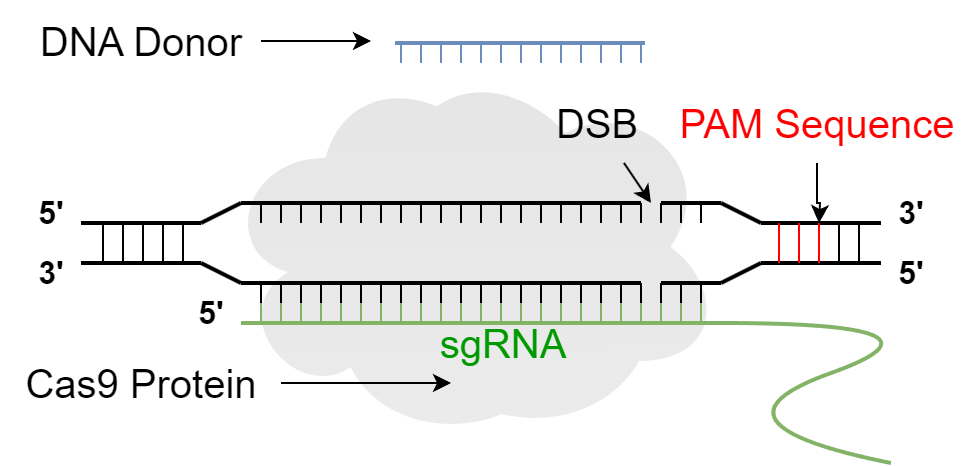
\includegraphics[width=0.46\textwidth]{dissertation-crispr-hdr.png}
        \label{fig:crispr-hdr}
    }
    \subfigure[Base Editor]{
        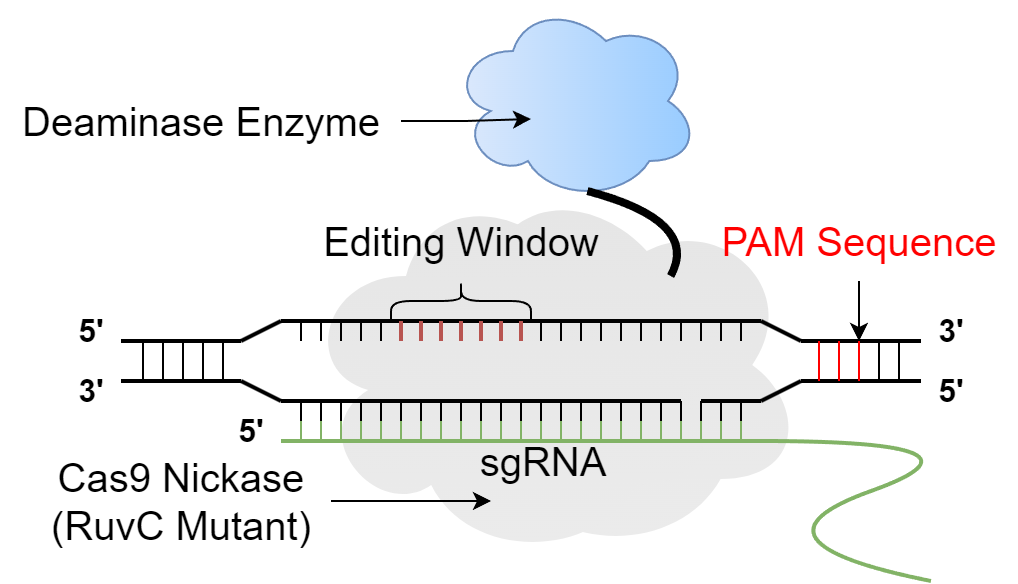
\includegraphics[width=0.46\textwidth]{dissertation-base-editor.png}
        \label{fig:base-editor}
    }
    \caption{Components for \textbf{(a)} CRISPR-Cas9 HDR  and \textbf{(b)} Base Editor  systems. The directions of DNA and RNA are denoted by 3' and 5' ends, based on the numbering of carbon atoms in the deoxyribose molecule (sugar group) forming the backbone of the DNA. The 5' end refers to the end where the phosphate  group attaches to the fifth carbon atom of the deoxyribose, while the 3' end refers to the end where the hydroxyl group  attaches to the third carbon atom.}
    \label{fig:crispr-base-editor}
\end{figure}

To avoid the inefficiencies produced by DSB while still leveraging the targeting capabilities of CRISPR system, the nickase versions of Cas9 proteins were developed. Cas9 nickase is a mutated version of the Cas9 protein that only cleaves the binding(RuvC mutation) or opposite(HNH mutation) strand of the guide RNA\cite{dasCRISPRBasedTherapeutics2022}. David Liu and his team developed the base editing system that uses the RuvC mutated Cas9 nickase to introduce point mutations in the genome, shown in Figure \ref{fig:base-editor}\cite{gaudelliProgrammableBaseEditing2017}. The base editing system consists of a fusion protein of the Cas9 nickase and a deaminase enzyme, and a sgRNA that guides the fusion protein to the target site. The deaminase enzyme converts a specific nucleotide within the editing window to another, and the Cas9 nickase introduces a nick in the non-edited strand to encourage the cell's endogenous repair machinery to use the edited strand as a template and permanently install the edit into the genome.

The base editors have been improved to be able to introduce point mutation within the editing window with relatively high efficiency\cite{portoBaseEditingAdvances2020}. However, they are only designed to introduce single-nucleotide variants into DNA or RNA, and are not capable of inserting and deleting sequences. To address this limitation and acquire a truly versatile genome editing tool, Liu's lab further developed prime editors\cite{liudavidr.SearchandreplaceGenomeEditing2019}. Prime editors are capable of introducing all 12 possible types of point mutations, as well as insertion and deletion of sequences up to a couple thousand base pairs in length\cite{linHighefficiencyPrimeEditing2021}. 

Prime editors consist of a fusion protein of SpCas9 (Streptococcus pyogenes) nickase and a MMLV reverse transcriptase, as well as a prime editing guide RNA (pegRNA), illustrated in Figure \ref{fig:prime-editor}. The SpCas9  nickase is a popular variant of Cas9 protein in recent years, mostly due to its high targetability (recognizing the common NGG PAM sequence, where N can be any nucleotide) and low off-target effects\cite{waltonUnconstrainedGenomeTargeting2020}. Similar to the sgRNA used by base editors, the pegRNA contains a nicking single guide RNA (ngRNA) at the $5'$ end. On the $3'$ end, however, pegRNA has a unique RNA sequence that encodes the desired edit. The $3'$ sequence can be divided into two parts: the primer binding site (PBS) and the reverse transcription template (RTT) consists of the intended edit surrounded by the left/right homology arms (LHA/RHA, RHA also called RTT overhang). As their names suggest, the PBS and RTT are used to prime the reverse transcription process, while the LHA and RHA are unedited sequences used to facilitate the integration of the edited sequence into the genome. The two ends of the pegRNA are connected by a crRNA scaffold sequence, which should have no participation in the prime editing process. 

\section{Process of Prime Editing}

\label{sec:prime-editing-process}

\begin{figure}[ht]
    \centering
    \subfigure[]{
        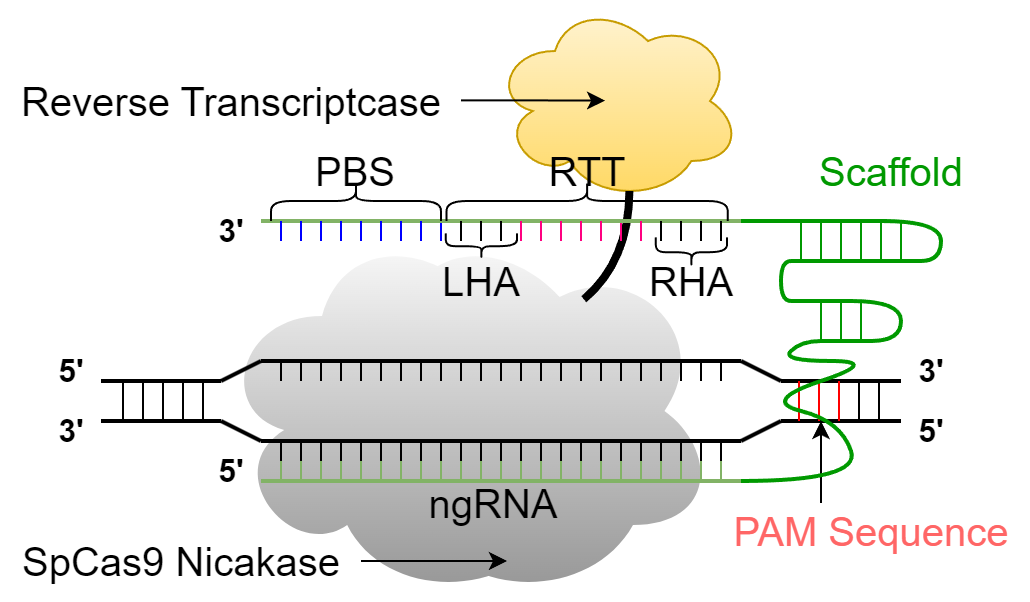
\includegraphics[width=0.46\textwidth]{dissertation-prime-editing-process-1.png}
        \label{fig:prime-editor}
    }
    \subfigure[]{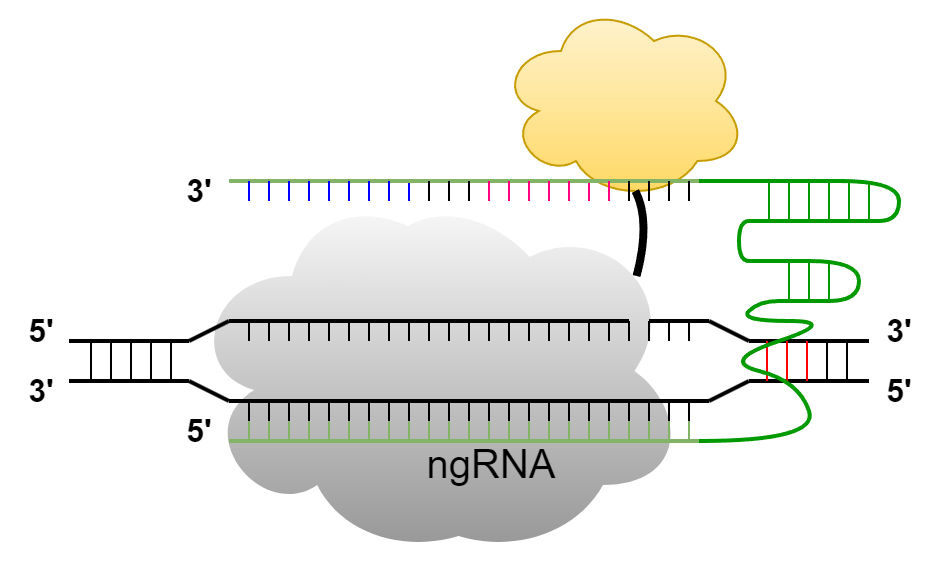
\includegraphics[width=0.46\textwidth]{dissertation-prime-editing-process-2.png}}
    \subfigure[]{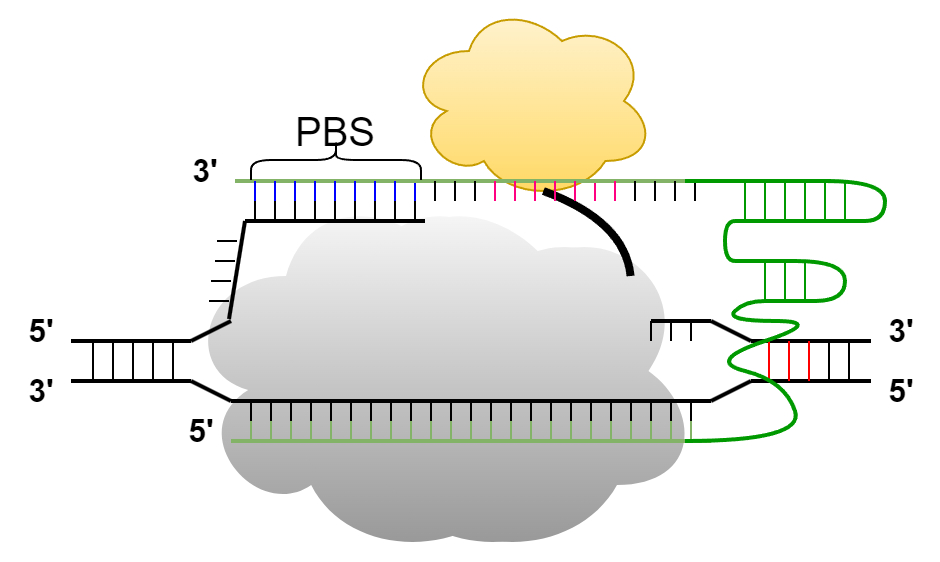
\includegraphics[width=0.46\textwidth]{dissertation-prime-editing-process-3.png}}
    \subfigure[]{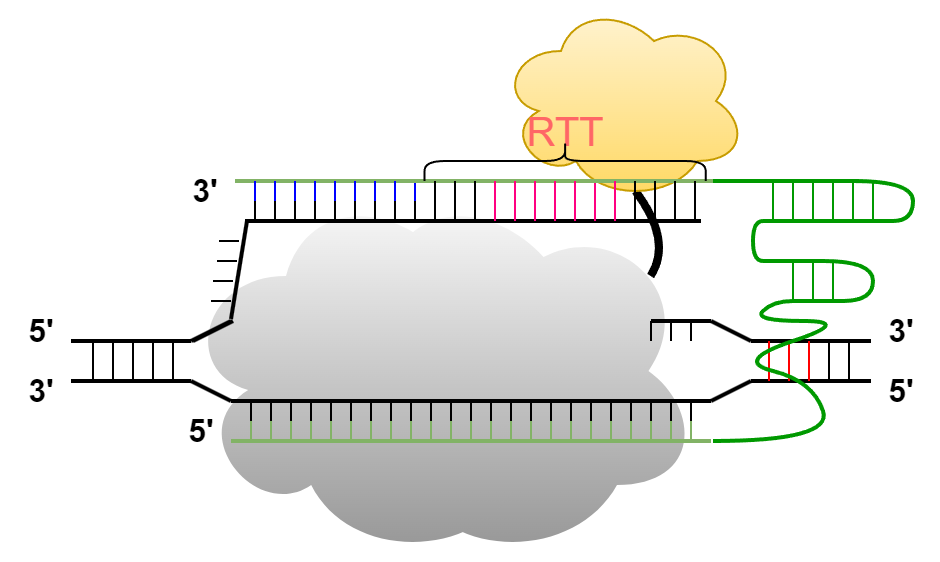
\includegraphics[width=0.46\textwidth]{dissertation-prime-editing-process-4.png}}
    \subfigure[]{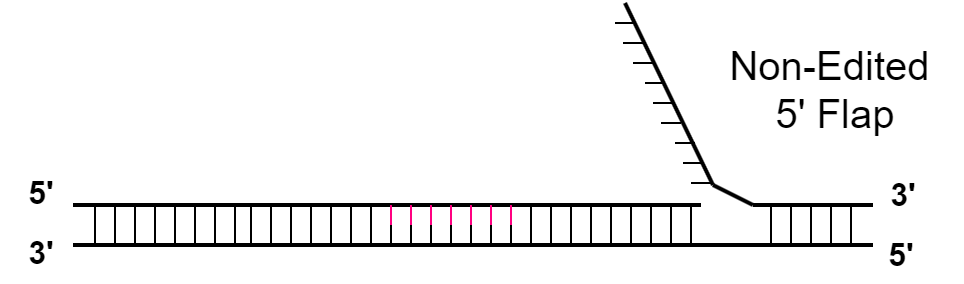
\includegraphics[width=0.46\textwidth]{dissertation-prime-editing-process-5.png}}
    \subfigure[]{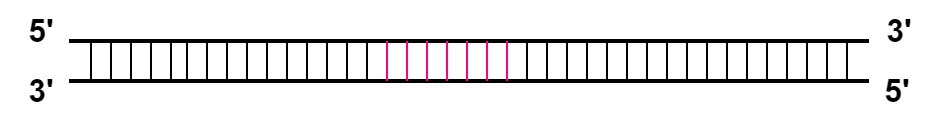
\includegraphics[width=0.46\textwidth]{dissertation-prime-editing-process-6.png}}
    \caption[Components of Prime Editor \textit{(a)} and the process of prime editing \textit{(a-f)}]{Components of Prime Editor \textit{(a)} and the process of prime editing \textit{(a-f)}: \textbf{(a)} ngRNA binds to the target DNA loci; \textbf{(b)} SpCas9 introduces nick 3-4 bp upstream of PAM; \textbf{(c)} The now exposed strand hybridizes with the PBS sequence in the pegRNA; \textbf{(d)} The RTT in the pegRNA is reverse transcribed into the target DNA; \textbf{(e)} The edited strand anneals to the non-edited strand; \textbf{(f)} The endogenous repair machinery incorporates the edited strand into the genome.}
    \label{fig:prime-editing-process}
\end{figure}

Numerous prime editors has been developed since the first generation(PE2, PE3) was introduced in 2019, including PE4 and PE5 with additional MLH1dn protein to inhibit the adverse mismatch repair pathway, as well as PE2-max and PE4-max with updated SpCas9 and reverse transcriptase\cite{liuPrimeEditingPrecise2023}. Despite their differences, all of the prime editors follow a similar multi-stage process illustrated in \autoref{fig:prime-editing-process}. 

The prime editing process starts with the denaturing (separation of the two strands) of target DNA loci. This allows ngRNA to bind to the complementary sequence immediately upstream of the protospacer adjacent motifs (PAM) required for successful annealing (binding of two complementary strands of DNA or RNA). The Cas9 nickase can then nick the exposed strand of the target DNA, creating a floating 3' end that can be used as a primer for the reverse transcription process. The PBS sequence in the pegRNA binds to the exposed 3' end, priming the reverse transcription of the RTT. 

Both the reverse transcribed 3' flap and non-edited 5' flat could anneal to the protospacer, and would result in a equilibrium of 3' and 5' flaps. If the edited 3' flap was excised, target would not be edited and can be processed again with prolonged editing. If the 5' flap was correctly excised, then we move on to the final step where the endogenous cellular repair system permanently incorporates the edited strand into the genome by repairing the mismatched base pairs. To stimulate the replacement of the non-edited strand, PE3 and PE5 have an additional sgRNA that guides the PE2 enzyme to nick the non-edited strand.

The reverse transcription mechanism gives prime editors an additional advantage. It can change bases far (at least 33bp) from the site of nick, instead of the narrow editing window of base editors. This allows prime editors to have lower constraint on the relative location of the PAM sequence, further increasing the versatility\cite{liuPrimeEditingPrecise2023}.

\section{In-silico Prediction of Prime Editing Outcome}

\label{sec:motivation}

More than 6,000 disorders are known to be caused by various types of mutations in the genome, with around 300 new genetic disorders being discovered each year\cite{petraityteGenomeEditingMedicine2021}. Due to its versatility, prime editing has the potential to correct up to 90\% of these disorder-inducing mutations\cite{kantorCRISPRCas9DNABaseEditing2020}, and the coverage is still increasing with new SpCas9 variants that have less and less PAM sequence constraints\cite{waltonUnconstrainedGenomeTargeting2020}. However, for prime editors to be useful in treating human diseases in clinical setting, it is crucial to have the highest possible accuracy with minimal off-target effects during the edits. 

The efficiency of prime editing can vary greatly across different target sites and pegRNA designs\cite{liudavidr.SearchandreplaceGenomeEditing2019}. Empirical approaches have been used to find the prime editor given a target edit, which involves testing a large number of combinations of ngRNA, PBS and RTT sequences repeatedly to find the optimal combination that yields the highest editing efficiency.

This is a laborious and time consuming process even for simpler editing tools such as base editors. With the more complicated process of prime editing, the search space is even larger. The lack of efficient optimization process can significantly limit the practicality in the clinical setting, especially in territories with an existing shortage of medical workers. As a result, in-silico optimization methods are highly desirable and has garnered the interest of many researchers.

Previous in-silico methods can be divided into two catagories: hypothesis driven models that use hard-coded rules to calculate the efficiency of a given edit\cite{hsuPrimeDesignSoftwareRapid2021,hwangPEDesignerPEAnalyzerWebbased2021}, and learning-based models that use machine learning to predict the editing outcome. 
The learning-based methods can be further divided into another two groups: the conventional machine learning methods that use hand-crafted features extracted from the sequence and prime editors\cite{liEasyPrimeMachineLearning2021,koeppelPredictionPrimeEditing2023}, as well as the deep learning methods that use the raw sequence data as part of their input\cite{yuPredictionEfficienciesDiverse2023,kimPredictingEfficiencyPrime2021, mathisPredictingPrimeEditing2023}. 

Each category has their own strengths and weaknesses in performance and efficiency. Hypothesis driven and conventional machine learning algorithms are more efficient to train due to the much smaller input size and the lower complexity of the computation. However, hypothesis based methods struggle to unbiasedly optimize the weights attributed to each feature\cite{liEasyPrimeMachineLearning2021}, while conventional machine learning algorithms loses the DNA context data that can be informative to prime editor optimization. 

The deep learning methods require a much larger dataset to train and are computationally more expensive to train and use. They also need more expertise to design and tune, and are more prone to overfitting due to the large number of parameters. However, their superior performance in the prime editing efficiency prediction task has been convincingly demonstrated by a number of models in recent years.

% TODO: overview of DeepPE, DeepPrime, PRIDICT 1 and 2

\subsection{DeepPE and DeepPrime convolutional neural network}

\begin{figure}
    \centering
    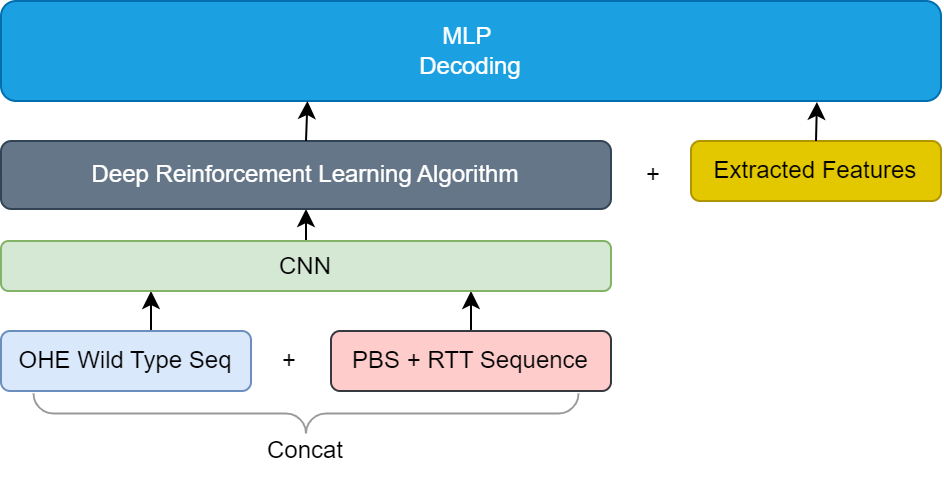
\includegraphics[width=0.7\textwidth]{DeepPE-simplified.png}
    \caption[DeepPE architecture]{DeepPE architecture. The input to the CNN is the one-hot encoded wild type and mutated DNA sequences concatenated with the extension RNA sequence. The output of the CNN is concatenated with the extracted features from the pegRNA sequence and the target site, and fed into the final MLP to predict the editing efficiency. Note that a deep reinforcement learning model was used here instead of a pooling layer to maintain local context information.}
    \label{fig:deeppe}
\end{figure}

DeepPE (\autoref{fig:deeppe}) was one of the earliest attempts at leveraging deep learning to achieve above par performance in predicting prime editing outcomes\cite{kimPredictingEfficiencyPrime2021}. It is a convolutional neural network (CNN) that takes the stacked one-hot encoded wild type and  mutated DNA sequences, the extension RNA sequence as well as a number of features extracted from pegRNA sequence and the target site as input. Despite its simple architecture, DeepPE managed to outperform the conventional machine learning models in terms of Pearson's r and Spearman's R. This indicated that the deep learning model was able to better capture the complex interactions between the sequence data and the editing efficiency compared to using the extracted features alone. It was however very limited in terms of the types of edits it can predict, with the base model only capable of predicting the efficiency of G to C replacement at 5bp upstream of the nick. Additional models were trained to predict other types of edits, and most of them also only support one single specific edit.

\begin{figure}
    \centering
    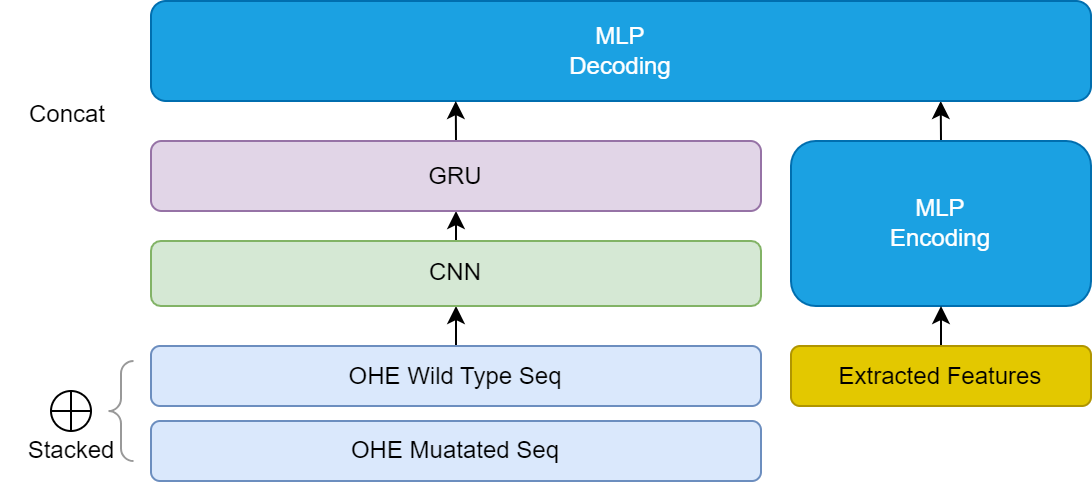
\includegraphics[width=0.85\textwidth]{DeepPrime-simplified.png}
    \caption[DeepPrime architecture]{DeepPrime architecture, updated from DeepPE. The CNN now uses a more conventional pooling layer, followed by a RNN GRU (Gated Recurrent Unit). The convolutional and recurrent layers take the stacked one-hot encoded wild type and mutated DNA sequences as input, and the output is concatenated with the extracted features processed by a MLP module. The concatenated output is then fed into another MLP to predict the editing efficiency.}
    \label{fig:deepprime}
\end{figure}

DeepPrime is a further attempt made by the same group to improve the performance and capabilities of DeepPE, leveraging the much bigger dataset as well as an improved architecture design\cite{yuPredictionEfficienciesDiverse2023}.
Noticing that stacking the additional PBS-RTT sequence did not improve the performance of DeepPE and added further constraint on pegRNA design (CNN only accept fixed length input), DeepPrime only used the wild type and mutated sequences as input to the deep learning model, and added a separate MLP (Multi Layer Perceptron) to process the computed features instead of directly concatenated the features onto the CNN output as DeepPE did. The output of the MLP was then concatenated with the output of the CNN that processed the sequence data, and fed into the final MLP to predict the editing efficiency. 

DeepPrime achieved far superior performance to DeepPE, while at the same time, one single model can now predict all types of edits for a cell line and prime editor pair existing in the dataset. This enabled the training process to take advantage of the shared features between different edits (further enhancing performance) and significantly improve the ease of use.

\subsection{PRIDICT 1 and 2 bidirectional GRU}

At around the same time DeepPrime was published, the PRIDICT model was developed by Mathis et al from the Schwank lab at the University of Zurch, and used RNN (Recurrent Neural Network) instead of CNN to process the sequence data\cite{mathisPredictingPrimeEditing2023}. The model uses a bidirectional GRU (Gated Recurrent Unit) to process the sequence data, whose output is pooled by a pair of global (whole sequence) and local (RTT region) attention(\autoref{fig:pridict}). Similar to DeepPrime, the features are encoded using a MLP and the output of the two models are then concatenated and fed into the final MLP to predict the editing efficiency.

\begin{figure}
    \centering
    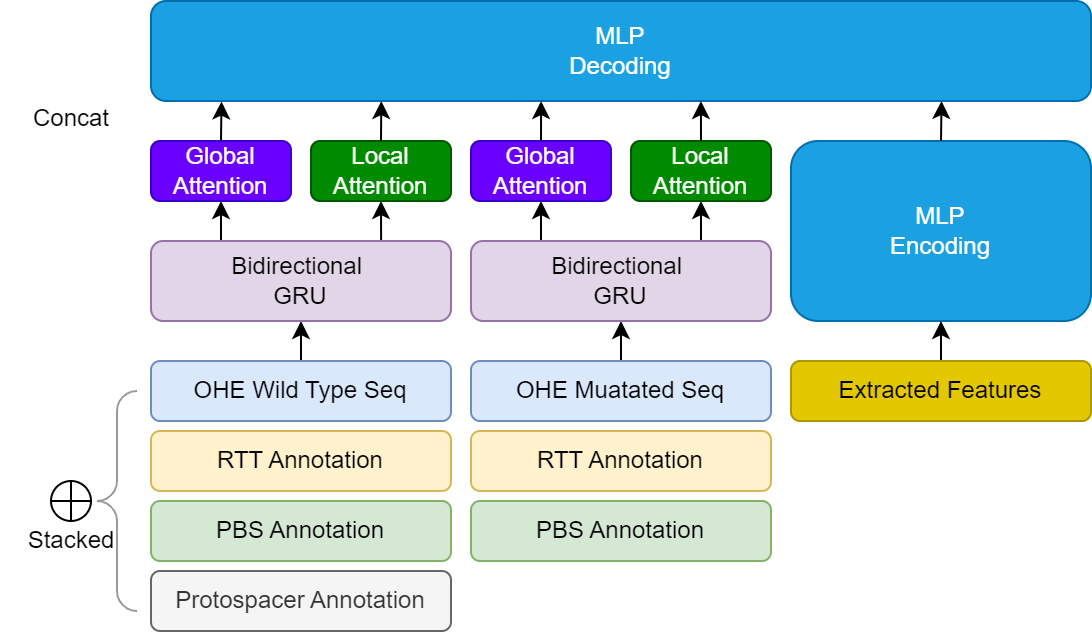
\includegraphics[width=0.85\textwidth]{pridict-simplified.png}
    \caption[PRIDICT architecture]{PRIDICT architecture. The input to the RNN is the one-hot encoded wild type and mutated DNA sequences, stacked with RTT, PBS, Protospacer(only for wild type) annotations. The annotation sequences are boolean sequences that indicate the functionality of each nucleotide in the sequence. The output of the RNN is processed by two attention heads, a global one that process the entire sequence and a local one that masks out all regions other than RTT. }
    \label{fig:pridict}
\end{figure}

This RNN based model was able to predict the efficiency of prime editing outcomes with up to 0.8 Pearson's r on their dataset, and was reported to be on par with the performance of DeepPrime.

Spurred by the success of the bidirectional RNN, the PRIDICT 2 model was developed by applying minor tweaks to the architecture as well as the data preprocessing steps and achieved even higher performance\cite{mathisMachineLearningPrediction2024}. More importantly, thanks to the far more diverse edits in the dataset with much longer inserts and deletes than the up to 3bp long edits in DeepPrime, PRIDICTv2 was more capable in the laboratory setting where insertion and deletions are reaching hundreds of base pairs in length\cite{liuPrimeEditingPrecise2023}.

\section{Study Objective}

(Rewrite)

The development of these models inspired me to further explore the potential of deep learning models in predicting prime editing outcomes. In this study, I aim to develop a deep learning model that is on par or even better than the existing models in predicting prime editing outcomes for a wide range of cell lines and edit types. 

I will also explore the possibility of using ensemble learning to improve the performance of the models, and investigate the potential of using the model to predict the efficiency of prime editing outcomes for cell lines and edit types that are not present in the training dataset. 

The best performing trained model would be presented as a web application that can be used by researchers to predict the efficiency of prime editing outcomes for their own cell lines and edit types.
\chapter{Methods}

\section{Curating a Benchmarking Dataset}

To establish a common ground for evaluating the performance of machine learning models, I curated a benchmarking dataset using data from various literatures. The main data source is the 2024 study by Mathis et al. which has the most diverse editing types ranging from 1-to-5bp replacement to 1-to-15bp deletions and insertions\cite{mathisMachineLearningPrediction2024}. It is complimented by the DeepPrime dataset, as it has a much bigger HEK293T dataset ($\sim290,000$ vs $\sim22,000$) as well as a wider range of cell type and PE pairs that can be used for fine-tuning the model to achieve better coverage and higher impact\cite{yuPredictionEfficienciesDiverse2023}. The mutated sequences in the datasets were masked by 'x', exposing only the region corresponding to PBS-RTT. To match the PRIDICT format, the mutated sequences were unmasked, and the missing regions due to the shorter wide sequence window is padded by `N'.


The dataset was parsed to preserve all essential information required by the models while also limiting the number of fields for better readability. More importantly, the standardized format allows easier conversion between datasets, with each data source requiring only two functions to allow universal usability, one to convert to and one to convert from standard format. The standard (std) format contains the following information:

\begin{itemize}[itemsep=-0mm]
    \item \textcolor{blue}{cell-line}: the cell line used in the experiment
    \item \textcolor{blue}{group-id}: the id of the target loci, used for grouping the data during cross validation
    \item \textcolor{blue}{mut-type}: the type of mutation introduced by the prime editor, 0 for replacements, 1 for insertions, 2 for deletions
    \item \textcolor{blue}{wt-sequence}: the 100bp/74bp long wild type target sequence starting from 10bp/4bp upstream of the protospacer(PRIDCT/DeepPrime dataset)
    \item \textcolor{blue}{mut-sequence}: the 100bp/74bp long edited target sequence starting from 4bp upstream of the protospacer(PRIDCT/DeepPrime dataset)
    \item \textcolor{blue}{protospacer-location}: the location of protospacer sequence complementary to sgRNA in the wild-type sequence 
    \item \textcolor{blue}{pbs-location}: the prime binding site
    \item \textcolor{blue}{rtt-location-wt/rtt-location-mut}: the location of reverse transcription template in the wild-type/edited sequence
    \item \textcolor{blue}{lha-location}: the location of left homology arm
    \item \textcolor{blue}{rha-location-wt/rha-location-mut}: the location of right homology arm in the wild-type/edited sequence
    \item \textcolor{blue}{spcas9-score}: precalculated SpCas9 score
    \item \textcolor{blue}{editing-result}: empirically observed editing efficiency
\end{itemize}

The locations are separated into two columns in the format of "start:end", where start is the 0-based index of the first base of the sequence, while end is for last base of the sequence(non-inclusive). All sequences were read in the direction of from protospacer to PAM for easier interpretation. This is often different from previous studies that read from 5' end to the 3' end of the pegRNA instead of using their relative position to the target sequence.

The data files are named as ``\{format\}-\{source\}-\{cell-line\}-\{PE-version\}.csv". `format' can be `std' for standard format, `shap' for files with only extracted features, as well as formats for individual models containing all the data required for training, such as `pd' for PRIDICT and `dp' for DeepPrime. `source' is the name of the study that the data was extracted from, while `cell-line' and `PE-version' are self explanatory.

Five main datasets of size greater than 10,000 were used frequently for benchmarking in this study: DeepPrime HEK293T PE2, PRIDICT2.0 HEK293T, PRIDICT2.0 K562, PRIDICT2.0 K562MLH1d, and PRIDICT2.0 Adv. The HEK293T cells refer to the human embryonic kidney cells\cite{kavsanImmortalizedCellsOne2011}; `Adv' refers to prime editing performed in-vivo (in a living organism) in mouse liver cells; K562 cells were derived from a chronic myelogenous leukemia patient\cite{lozzioMultipotentialLeukemiaCell1981} (K562MLH1d refers to K562 cells with MMR inhibition using the MLH1dn proteins). Other smaller datasets were used for fine tuning models trained with the DeepPrime HEK293T PE2 dataset, such as the DeepPrime HEK293T PE2-Max dataset.

The editing efficiencies were calculated using the method suggested by Kim et al.\cite{kimPredictingEfficiencyPrime2021} in \autoref{eq:efficiency}, which was also used by PRIDICT:
\begin{equation}
    \label{eq:efficiency}
    \begin{split}
        \text{Editing Efficiency} =& \frac{\text{Edited Count}}{\text{Total Count}} \times 100\% \\
    \end{split}
\end{equation}
Where:
\begin{equation}
    \begin{split}
        \text{Edited Count} =& \text{Read Counts With Intended Edit at Target Site} - \\
        &( \text{Total Read Counts} \times \text{Background Editing  Rate} ) \\
        \text{Total Count} =& \text{Total Read Counts} - (\text{Total Read Counts} \times \\ &\text{Background Editing  Rate})
    \end{split}
\end{equation}
        
Background editing rate refers to the percentage of target loci that were edited without being transfected with the prime editor. Subtracting the background edits from the total read counts gives the estimated true number of reads that were edited by the prime editor.

The datasets are split into 5 folds based on the group id assigned to each target loci and pegRNA combination. Edits on the same target loci have the same group id, and are thus placed in the same fold to prevent data leakage. The folds are then used for cross validation to evaluate the model's performance.



\section{Determinants of Prime Editing Outcome}
\label{sec:determinants}

\begin{figure}
    \centering
    \subfigure[DeepPrime]{
        \label{fig:shap-dp-pe2-hek}
        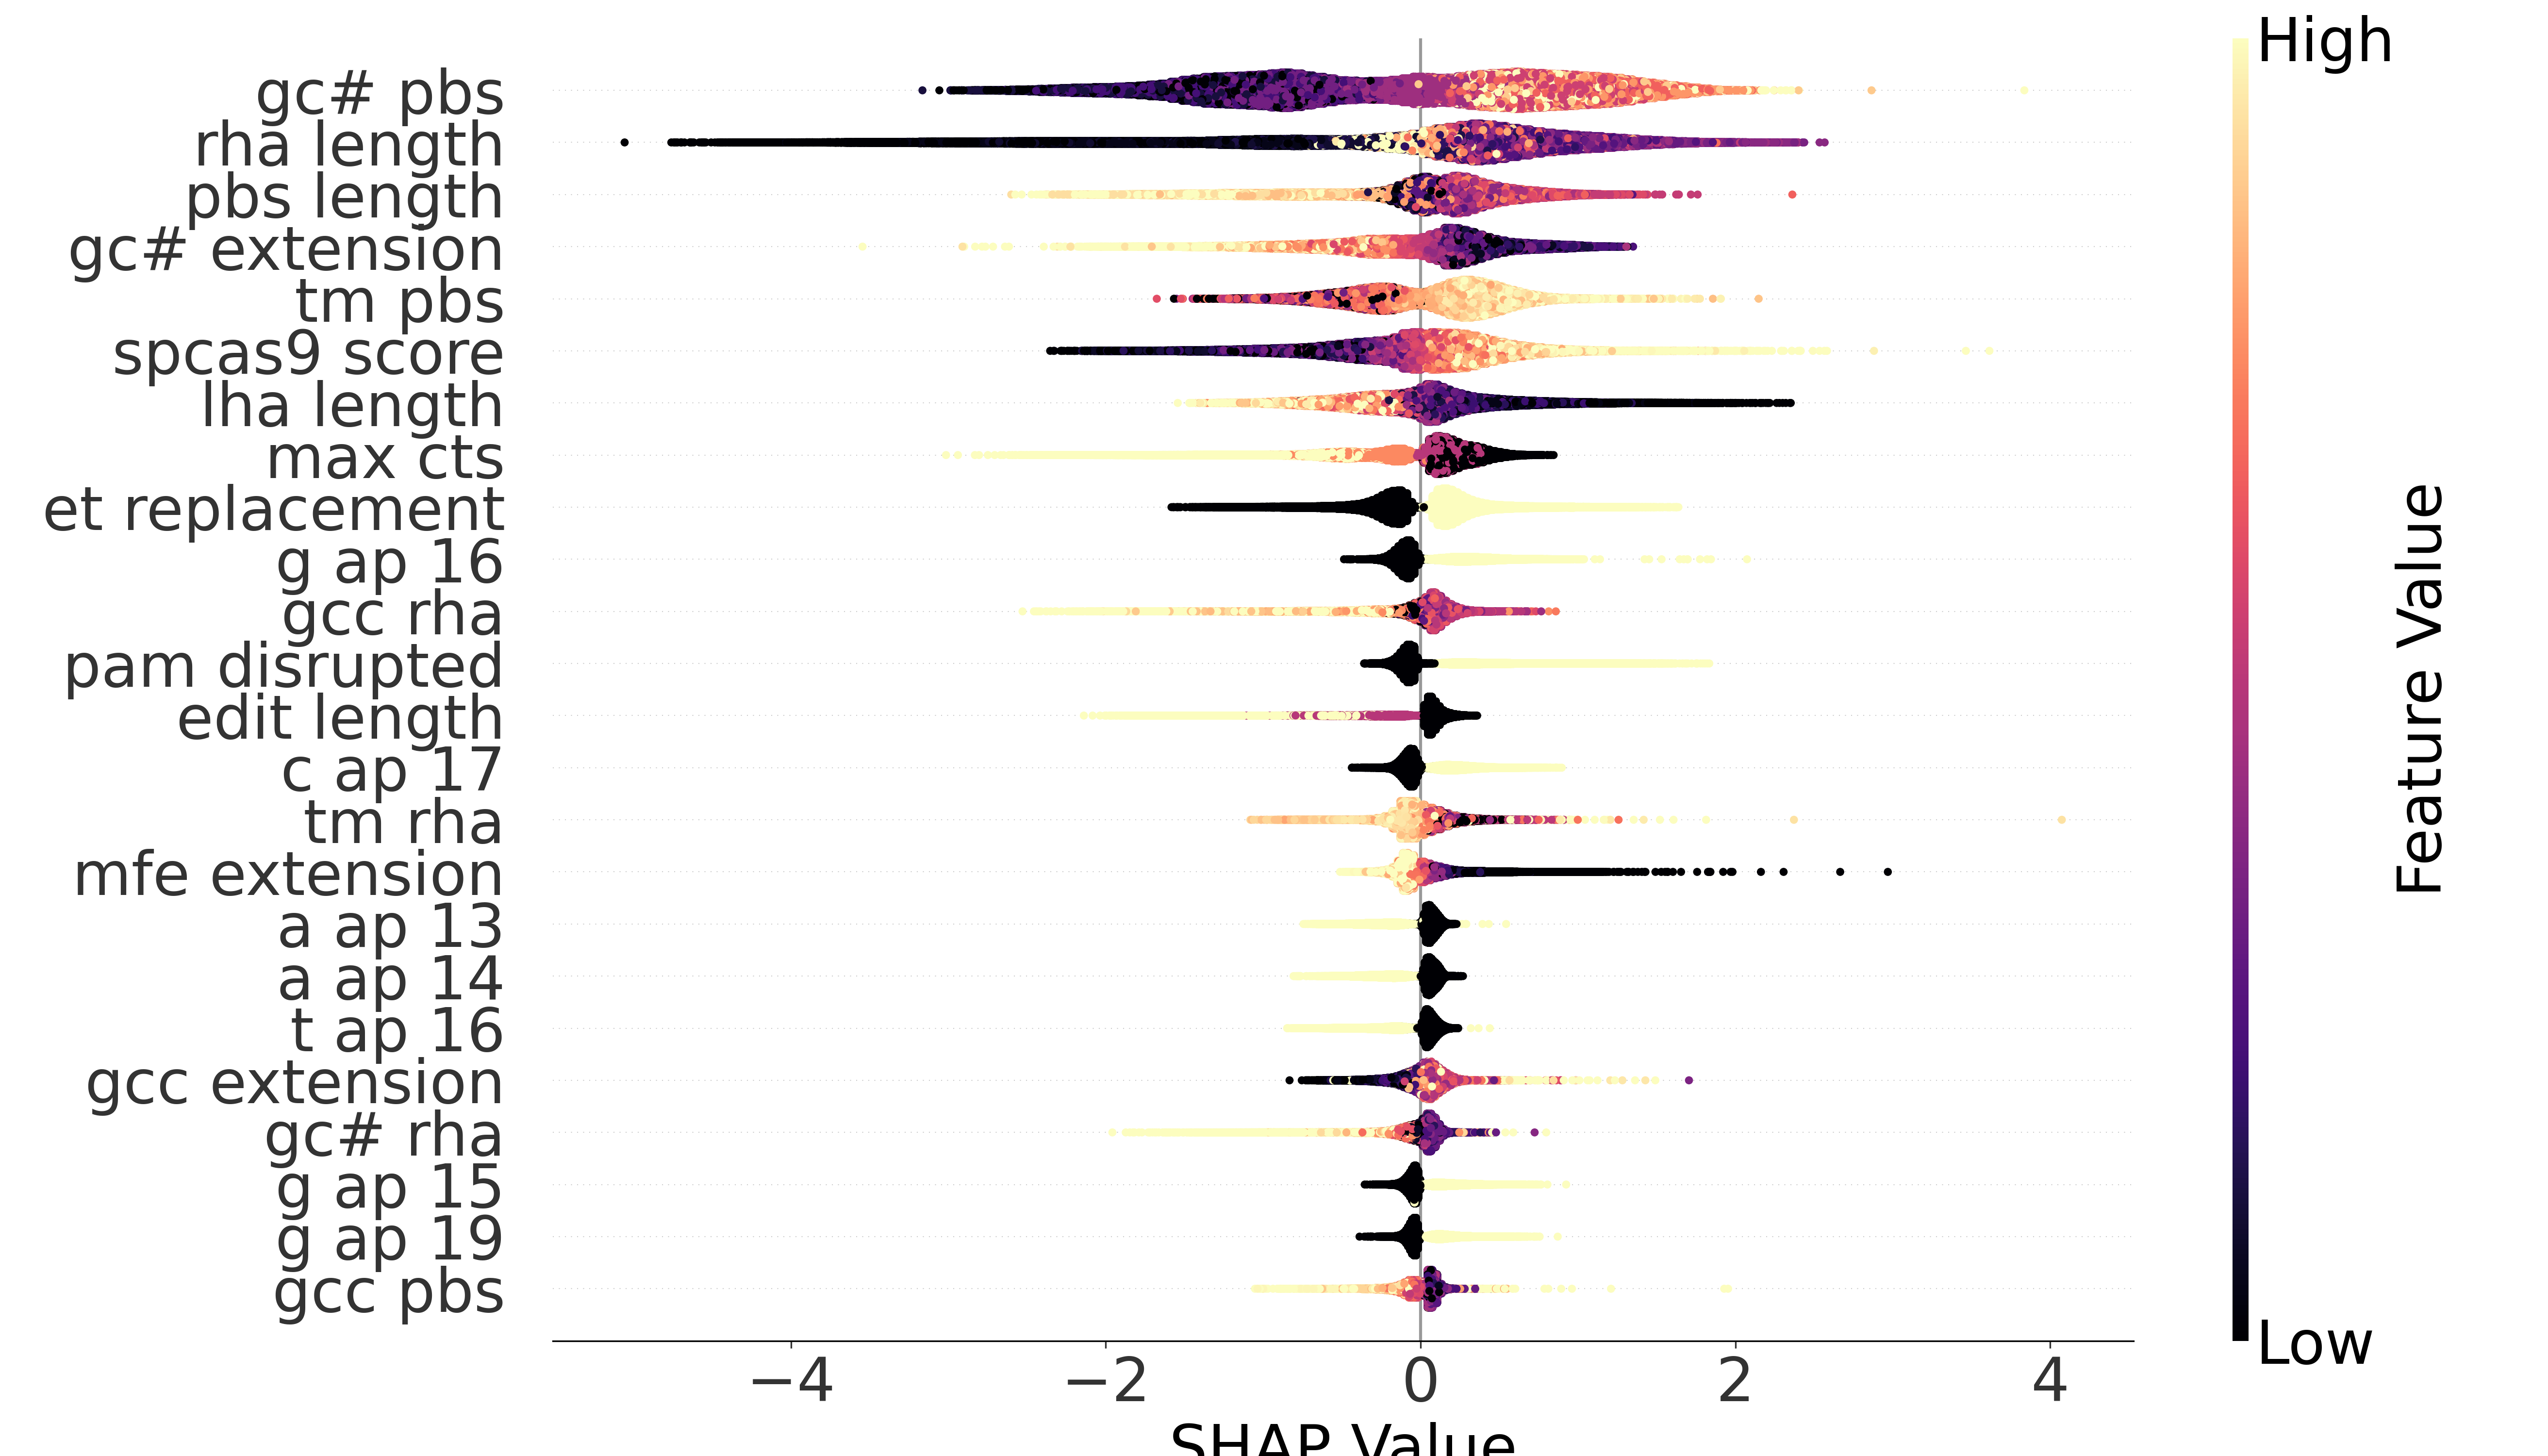
\includegraphics[width=0.99\textwidth]{shap-dp-hek293t-pe2.png}}
    \subfigure[Deletion]{
        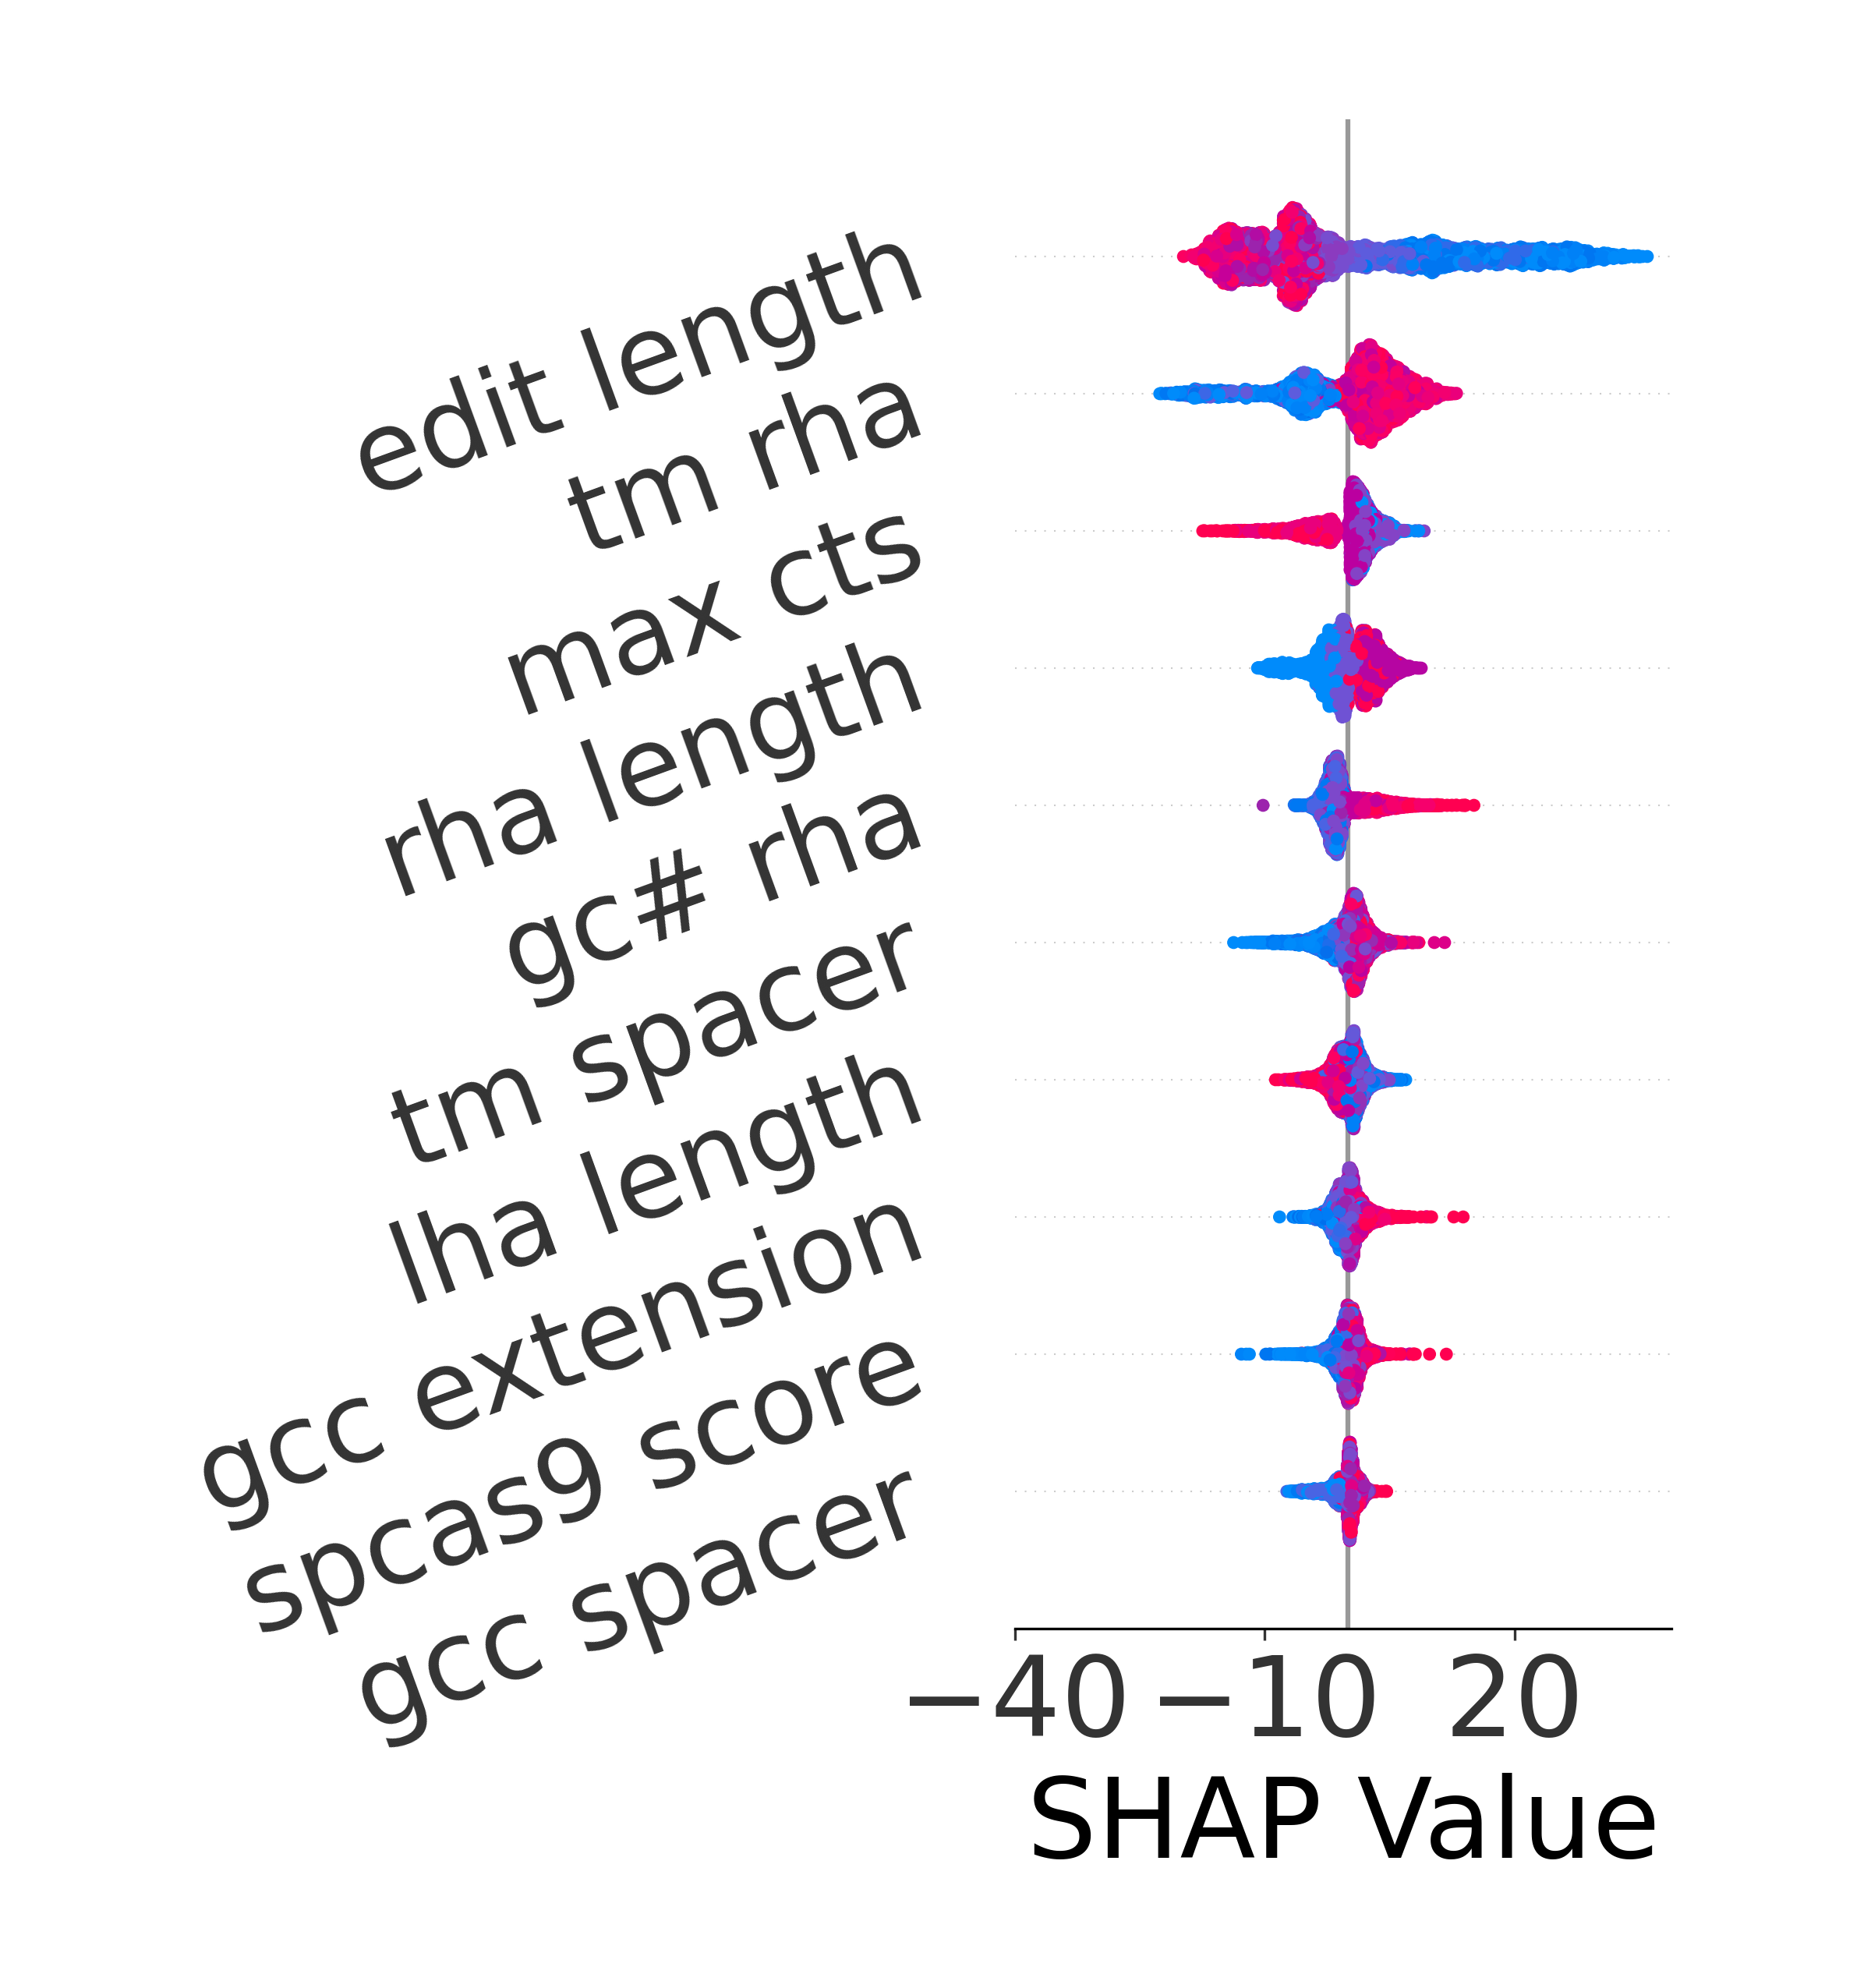
\includegraphics[width=0.3\textwidth]{shap-pd-hek293t-pe2-delete.png}
    }
    \subfigure[Insertion]{
        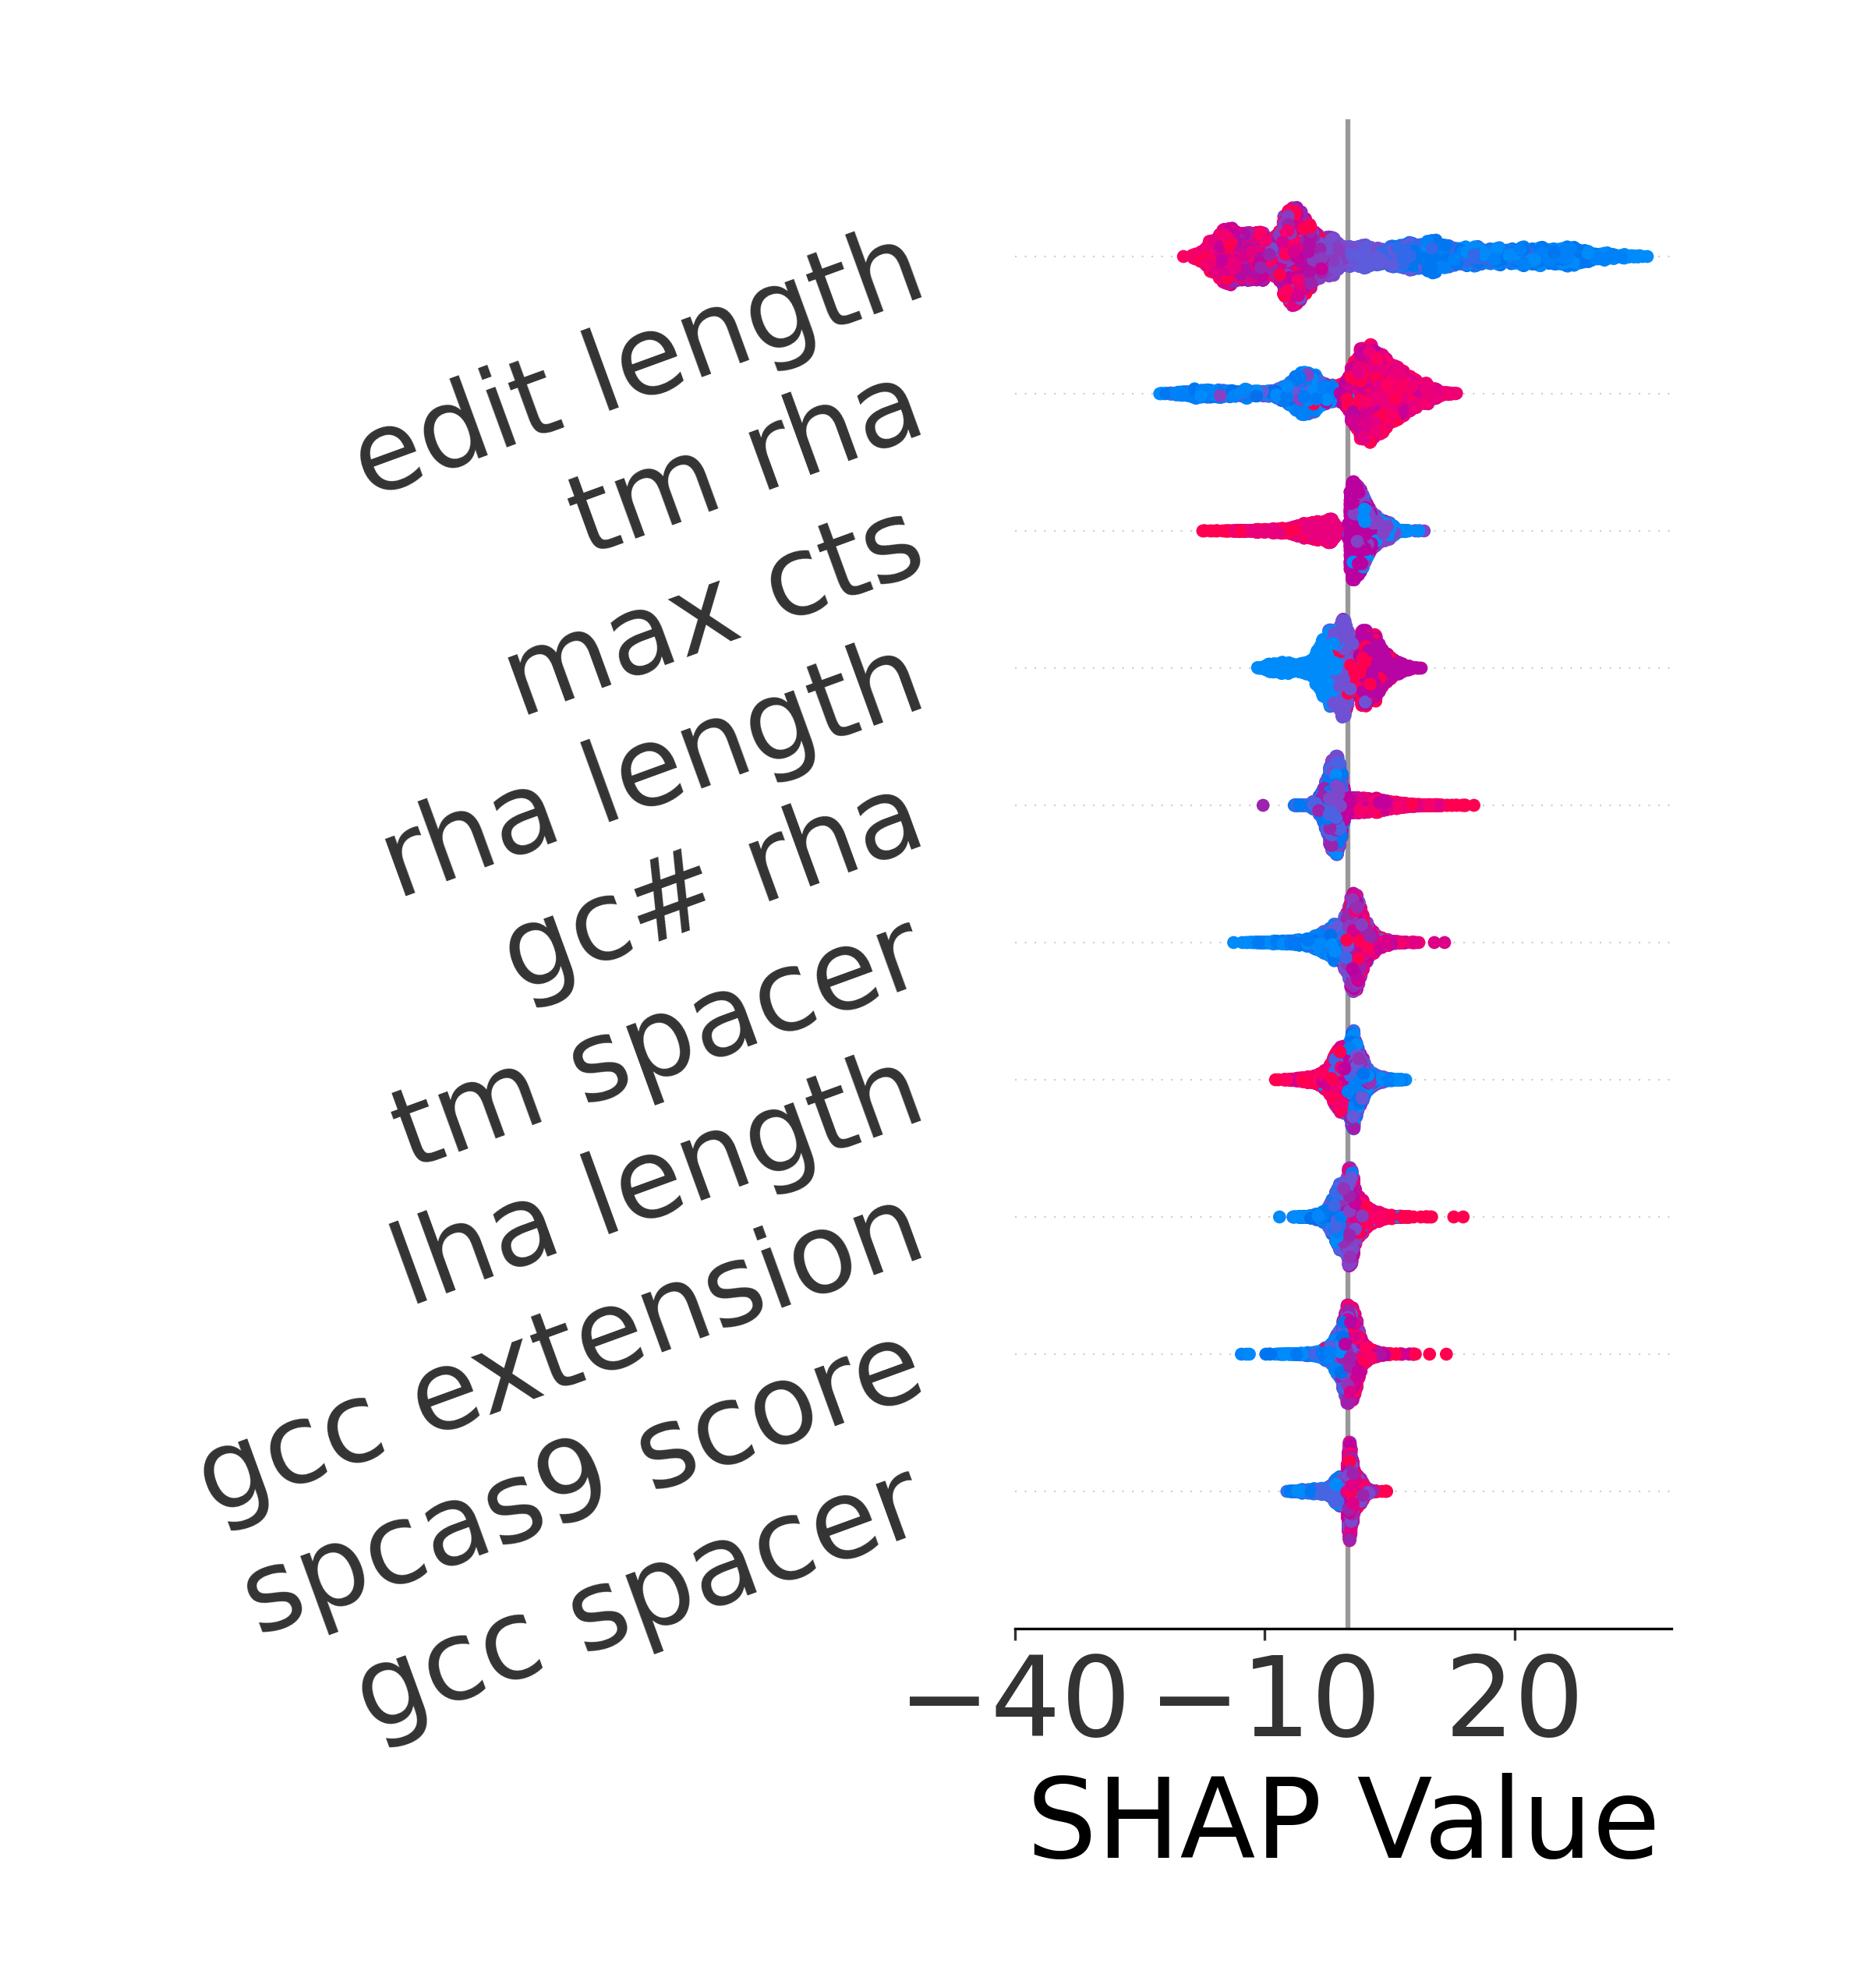
\includegraphics[width=0.3\textwidth]{shap-pd-hek293t-pe2-insert.png}
    }
    \subfigure[Replacement]{
        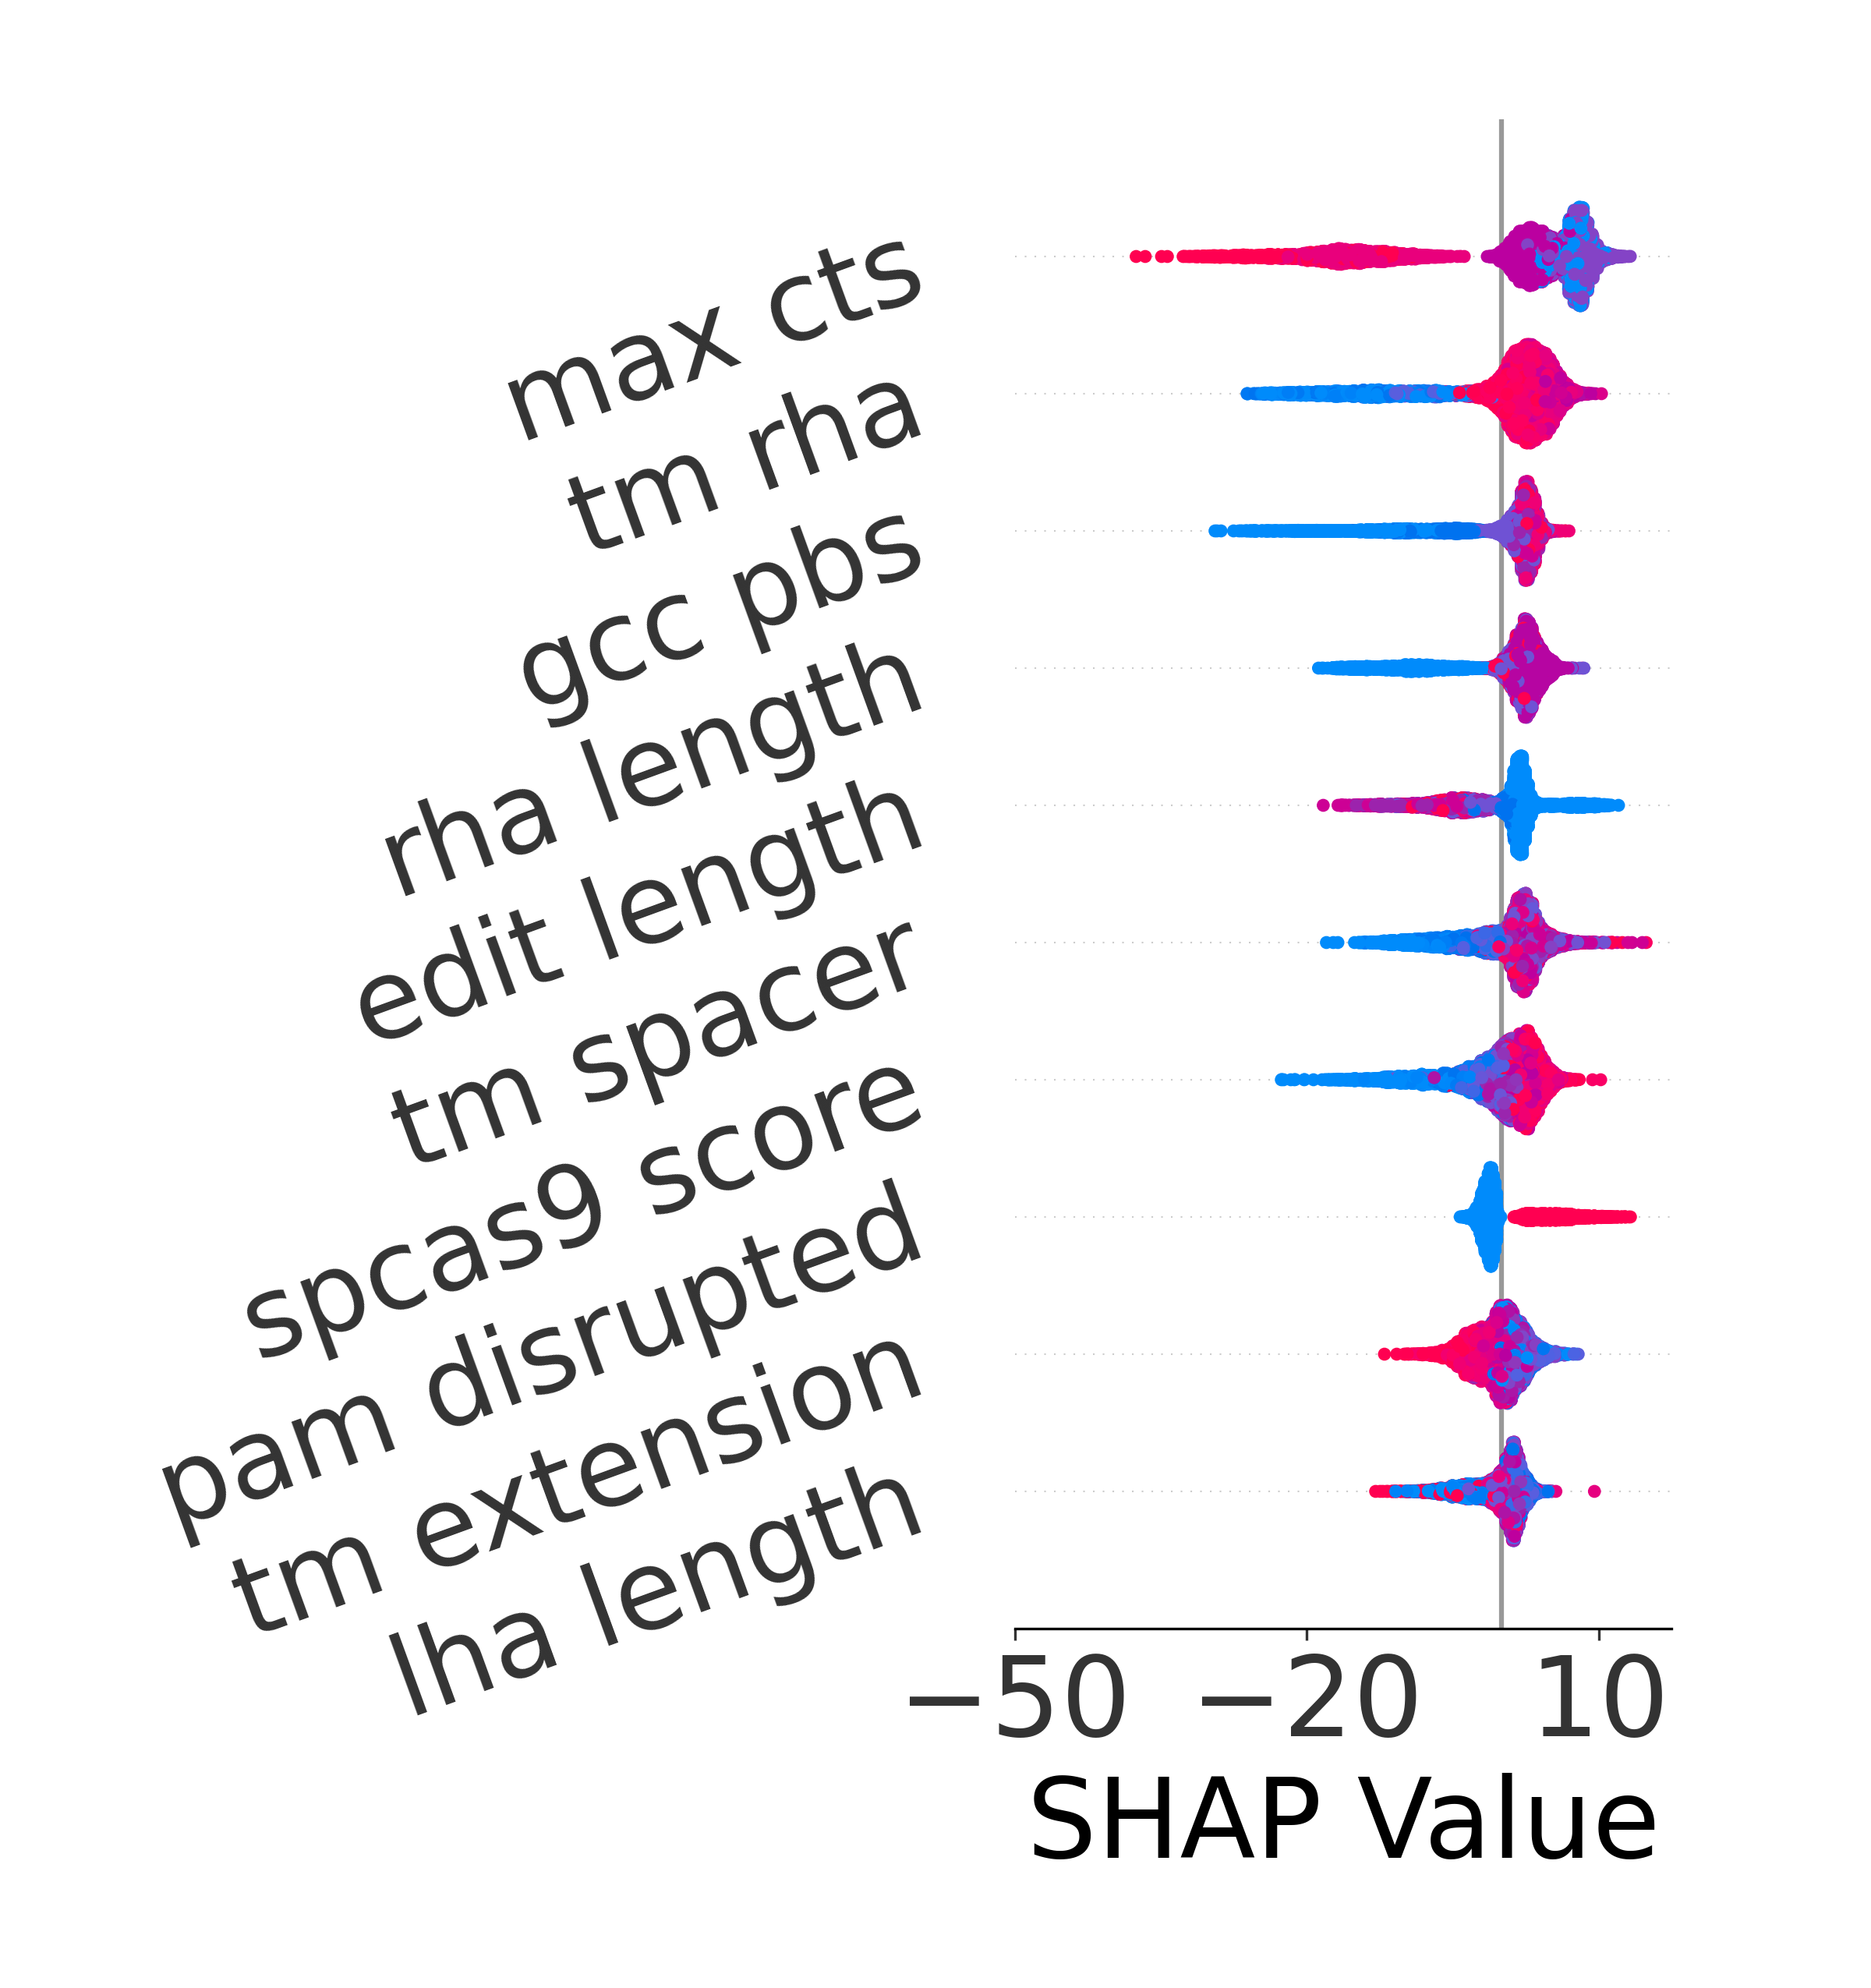
\includegraphics[width=0.3\textwidth]{shap-pd-hek293t-pe2-replace.png}
    }
    \caption[SHAP analysis for DeepPrime and PRIDICT2.0 datasets on HEK293T cell line.]{SHAP analysis for DeepPrime and PRIDICT2.0 datasets on HEK293T cell line: \textbf{(a)} Top 15 determinants from SHAP analysis using all of DeepPrime HEK293T Datasets. \textbf{(b-d)} Top 10 determinants from SHAP analysis using PRIDICT2.0 HEK293T data for each individual editing types. The colour of the individual data point shows their normalized values from high (red) to low (blue). The binary values have 1 (True) for high and 0 (False) for low. A number of shorthands have been used to improve the clarity of the illustrations. gcc for GC Content (different from GC count); et for editing type; tm for melting temperature; mfe for minimum free energy; n ap \# for base n at protospacer position \#; max cns for the length of maximum consecutive sequence of base n.} 
    \label{fig:shap}
\end{figure}

As discussed in \autoref{sec:motivation}, most of the recent deep learning models surveyed in the literature (DeepPrime\cite{yuPredictionEfficienciesDiverse2023} and PRIDICT\cite{mathisPredictingPrimeEditing2023,mathisMachineLearningPrediction2024}) followed a similar two model structure. The first model is a deep neural network taking in raw sequence data, and the second model is a smaller MLP/regression model that takes as input the features extracted from the PBS, RTT and ngRNA. For single model architecture (DeepPE\cite{kimPredictingEfficiencyPrime2021}), the features are concatenated to the sequence data and fed into the model.

As a result, it is important to find the most prominent determinants of prime editing outcomes and to extract the most informative features for describing the pegRNA. A large number of features were selected from various sources as the studies focus on different aspects of pegRNA. Shapley Additive Explanations (SHAP) with XGBoost regressor to rank the features based on their importance. The full list of features investigated can be found in \autoref{appendix:features}. 

A number of Python libraries were utilized when extracting the features into the `shap' format. The melting temperature of the sequences were calculated using the 'biopython' library\cite{cockBiopythonFreelyAvailable2009}, the minimum free energy was calculated with the ViennaRNA package and adjusted using sequence length to ensure it's mostly influenced by sequence's nucleotide order and composition\cite{lorenzViennaRNAPackage2011,trottaNormalizationMinimumFree2014}, and the SpCas9 scores were provided by the 'DeepSpCas9' model\cite{kimSpCas9ActivityPrediction2019}. Other features such as GC content were extracted using simple Python string processing functions.

SHAP analysis was first conducted on the largest DeepPrime PE2 HEK293T dataset to provide the most robust identification of the most informative features (Figure \ref{fig:shap-dp-pe2-hek}). The features were then sorted based on their importance, and the top 24 features were used for the model, matching the design optimized by DeepPrime\cite{yuPredictionEfficienciesDiverse2023}. To identify the influence of the features on different editing types, SHAP analysis was also conducted on the PRIDICT2.0 HEK293T dataset for each individual editing type (\autoref{fig:shap}(b-d)), due to its higher variety of editing length. 

The major determinants are as follows:
\begin{itemize}[itemsep=-0mm]
    \item \textcolor{red}{Editing type and length}: editing type has a significant impact on the editing efficiency, with the replacement type having higher efficiency than the insertion and deletion, as shown by the `et replacement' feature in Figure \ref{fig:shap-dp-pe2-hek}. The length of the edit also has great influence on editing result, and its important is more pronounced for deletions and insertions than replacements. As expected, longer edits have lower efficiency due to the increased difficulty in the annealing and repair process.
    \item \textcolor{red}{Melting temperature}: melting temperature (Tm) refers to the temperature at which half of the RNA strand become unfolded or denatured. It is strongly correlated with the editing efficiency, possibly due to its influence on RNA structural stability. Its actual effect, however, is highly mixed. A low Tm in extension seems to positively affect the editing result, while the opposite is true for pbs. At the same time, high Tm in RHA has a mixed impact in the DeepPrime dataset (`tm rha' in Figure \ref{fig:shap-dp-pe2-hek}), while in the PRIDICT2\.0 dataset, high Tm in the PBS is clearly beneficial for the editing process of all types (`tm rha' in \autoref{fig:shap}(b-d)).
    \item \textcolor{red}{Minimum free energy}: minimum free energy (MFE) describes the lowest possible energy required for a RNA sequence to stay in a particular form\cite{lorenzViennaRNAPackage2011}. It appears to have similar effect to Tm, with low MFE in the extension being beneficial for the editing efficiency.
    % TODO: Check MFE 
    \item \textcolor{red}{GC content/count}: GC count in the PBS sequence was shown to be the most important feature for the DeepPrime dataset (Figure \ref{fig:shap-dp-pe2-hek}), consistent with the observation made by Liu et al in their 2019 study introducing prime editors\cite{liudavidr.SearchandreplaceGenomeEditing2019}. They expected lower editing efficiency with low GC count in the PBS, due to the energetic requirements of hybridization of the nicked DNA strand to the PBS. GC content also correlates to the minimum free energy and melting temperature, as GC base pairs have stronger hydrogen bond than AU base pairs.
    \item \textcolor{red}{Poly-T sequences}: Shown as `max cts' in \autoref{fig:shap}, the length of the longest consecutive T (poly-T) sequences in the cDNA of the 3'extension and spacer RNA sequences has a clear negative impact on the editing efficiency. The poly-T termination signal, while not causing termination in itself, causes catalytic inactivation and backtracking of Pol III\cite{nielsenMechanismEukaryoticRNA2013}
    \item \textcolor{red}{SpCas9 score}: DeepSpCas9 is a deep learning model that estimates the activity of the SpCas9 protein on a target loci, and has been shown to be a good indicator of prime editing efficiency\cite{kimPredictingEfficiencyPrime2021}. This is likely due the SpCas9's role in the prime editing process, as it is responsible for the initial binding of the pegRNA to the target loci. 
    \item \textcolor{red}{PAM disruption}: it was shown that prime editors can sometimes rebind to the edited sequences and induce unintended edits, lowering the editing efficiency\cite{liudavidr.SearchandreplaceGenomeEditing2019}. Thus, the disruption of the PAM sequence is beneficial for the editing efficiency as it prevents the reannealing of the pegRNA to the edited sequence.
    \item \textcolor{red}{LHA/RHA/PBS length}: the length of rha (right homology arm, RTT overhang) is a significant determinant for all editing types, with a short rha length leading to deceased prime editing efficiency, while the positive effect of a long rha is not as pronounced. This suggests the existence of a minimum threshold for rha length below which the edited strand cannot efficiently anneal to the unedited strand, consistent with the findings of Yu et al, 2023, recommending a rha length of at least 7nt\cite{yuPredictionEfficienciesDiverse2023}. Reported as edit position in some literatures, lha length corresponding to the distance between the PAM sequence and the edit location is also a significant feature for all editing types, especially insertion and deletion. A longer lha length adversely affects the editing efficiency, suggesting that although prime editors have less stringent requirements for PAM locations, editing should still be done close to the protospacer whenever possible. As for PBS length, both a very short and a very long PBS have a negative impact on the editing efficiency, suggesting an optimal range.
    \item \textcolor{red}{Protospacer nucleotide composition}: in Figure \ref{fig:shap-dp-pe2-hek}, a guanine nucleotide (G) at protospacer location 16 was shown to have a positive impact on the editing efficiency. On top of that, among the top 24 features, the nucleotide compositions from protospacer location 13 to 17 were all shown to have a significant impact. 
    % TODO explain why
\end{itemize}

On top of the quantitatively invested sequence based features, higher level features have also been shown to impact prime editing efficiency:
\begin{itemize}[itemsep=-0mm]
    \item \textcolor{red}{pegRNA secondary structure}: the secondary structure of the pegRNA can impact the efficiency by inducing degradation of the 3' extension. The defunct pegRNA can still combine with target loci using its functioning 5' ngRNA, thus lowering the editing efficiency\cite{nelsonEngineeredPegRNAsImprove2022}.
    \item \textcolor{red}{MMR Behaviour}: as briefly mentioned at the beginning of \autoref{sec:prime-editing-process}, the mismatch repair(MMR) system adversely affects the editing efficiency during step (e) of the prime editing process. The MMR system may reject the annealing of the editing strand to the target loci, or it may excise the edited sequence, preferring the original sequence\cite{chenEnhancedPrimeEditing2021}. 
\end{itemize}

These features are encapsulated in the editing cell type and PE version and are thus not explicitly included in the feature list. For example, epegRNAs(engineered pegRNA) are improved version of pegRNA that are designed for protection against 3' erosion with a more robust secondary structure than the original versions\cite{nelsonEngineeredPegRNAsImprove2022}. At the same time, PE4 and PE5 are newer versions of prime editors with MLH1dn proteins that can suppress the MMR system\cite{chenEnhancedPrimeEditing2021}, and the HEK293T cell line has weaker MMR activity than other cell lines such
as HAP1(derived from a chronic myelogenous leukemia patient)\cite{mathisPredictingPrimeEditing2023}. 

\section{Data Engineering}

A conspicuous issue with the dataset is the imbalance in target values. Shown in Figure \ref{fig:imbalanced-original}, the distribution of the editing efficiency is heavily skewed towards the lower end, with a large number of pegRNAs having an efficiency of around 0. This can cause the model to be less accurate in predicting the higher efficiency pegRNAs, as the model would be more inclined to predict lower efficiency to minimize the loss. 

\begin{figure}
    \centering
    \subfigure[Original]{
        \label{fig:imbalanced-original}
        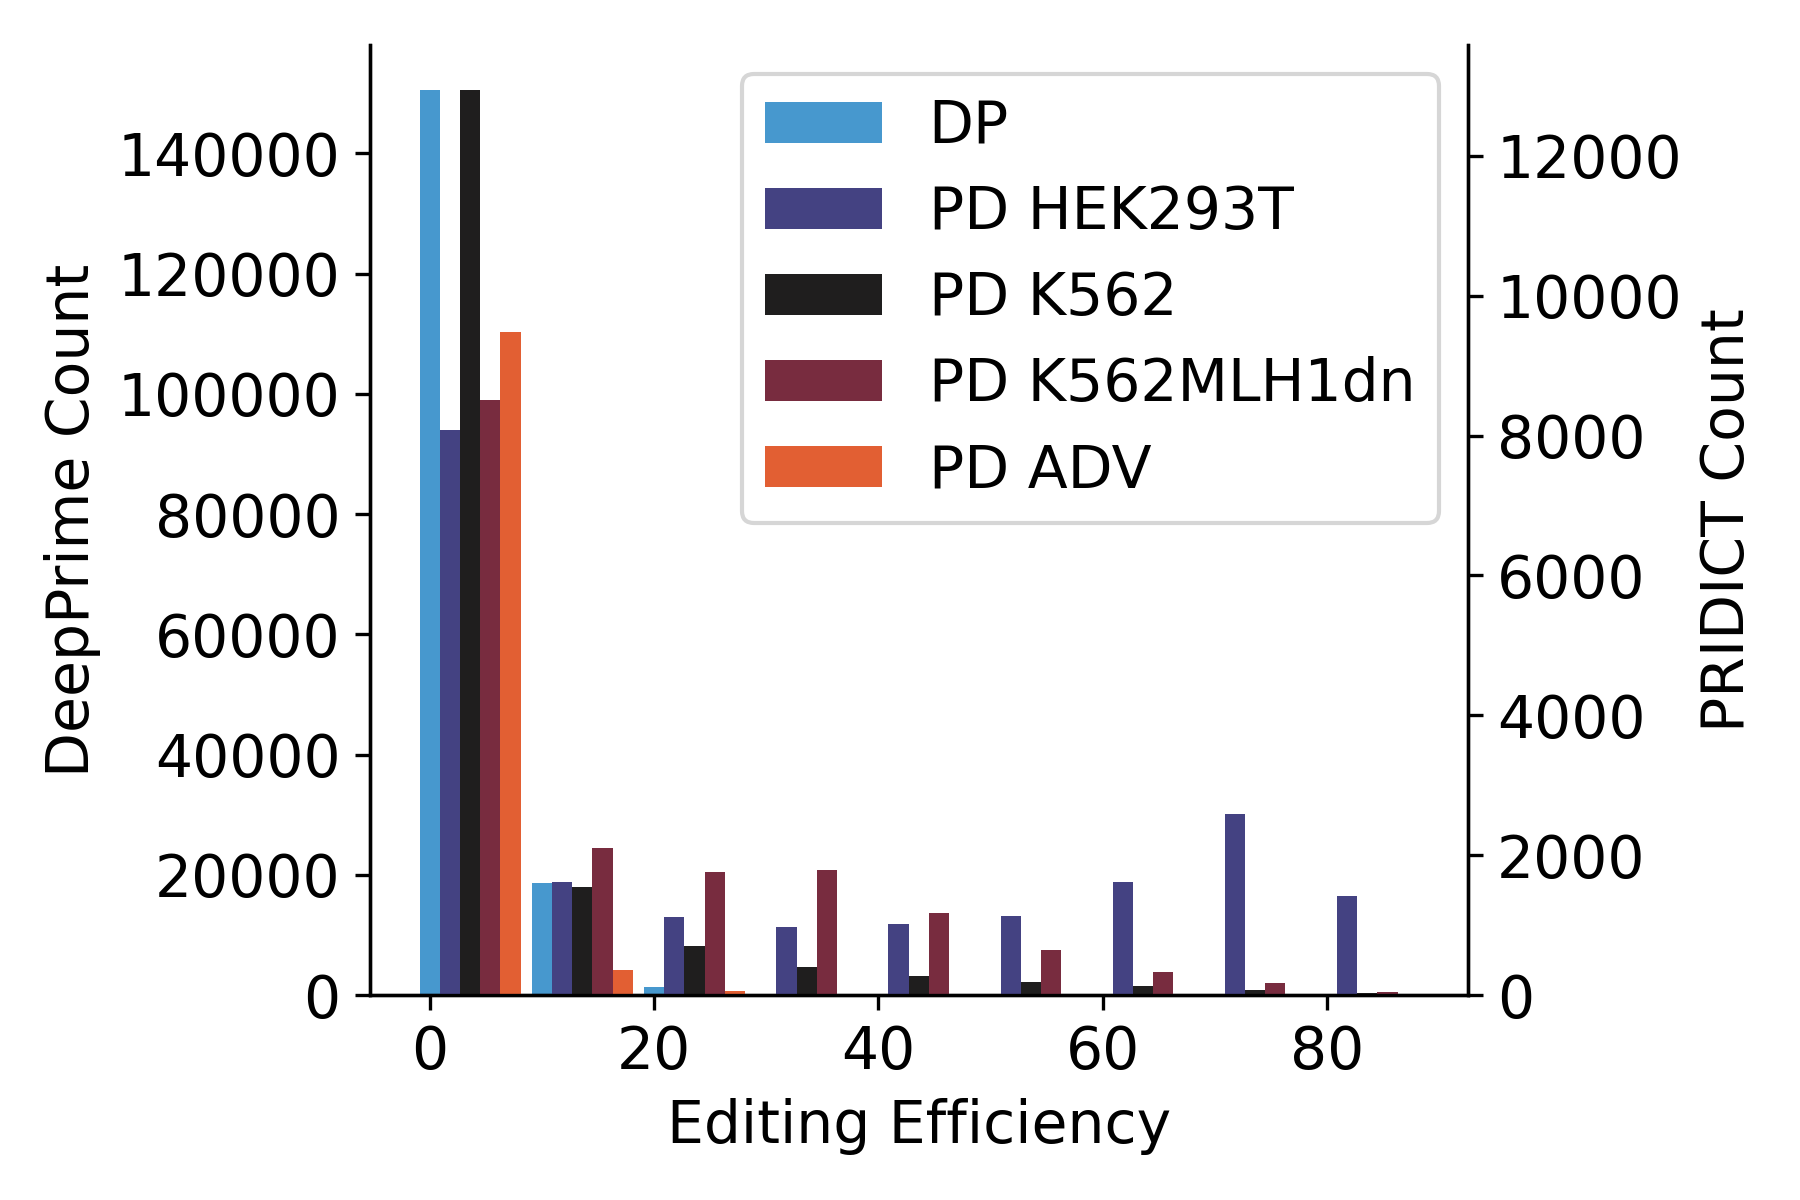
\includegraphics[width=0.45\textwidth]{editing-efficiency-comparison.png}
    }
    \subfigure[Log Adjusted]{
        \label{fig:imbalanced-log}
        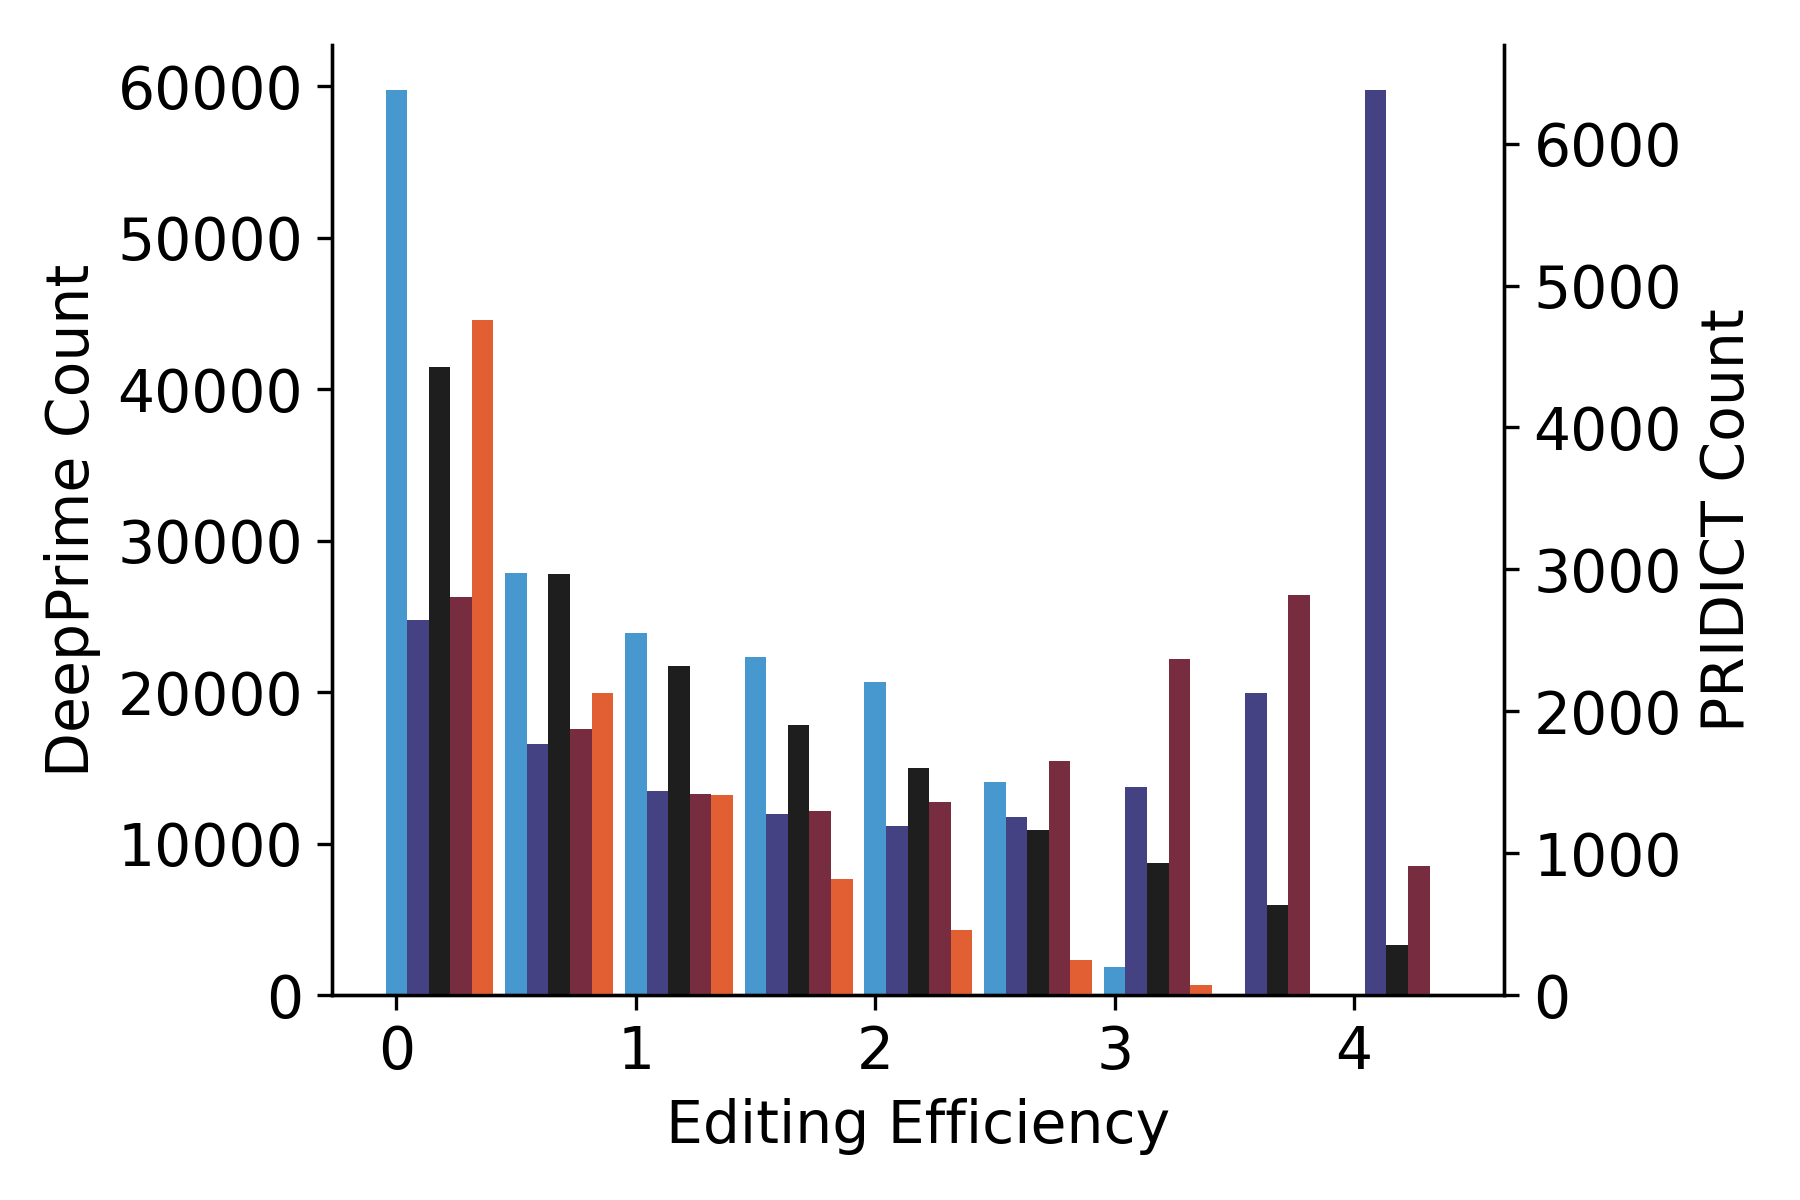
\includegraphics[width=0.45\textwidth]{editing-efficiency-log-adjusted.png}
    }
    \subfigure[Undersampling]{
        \label{fig:imbalanced-undersampling}
        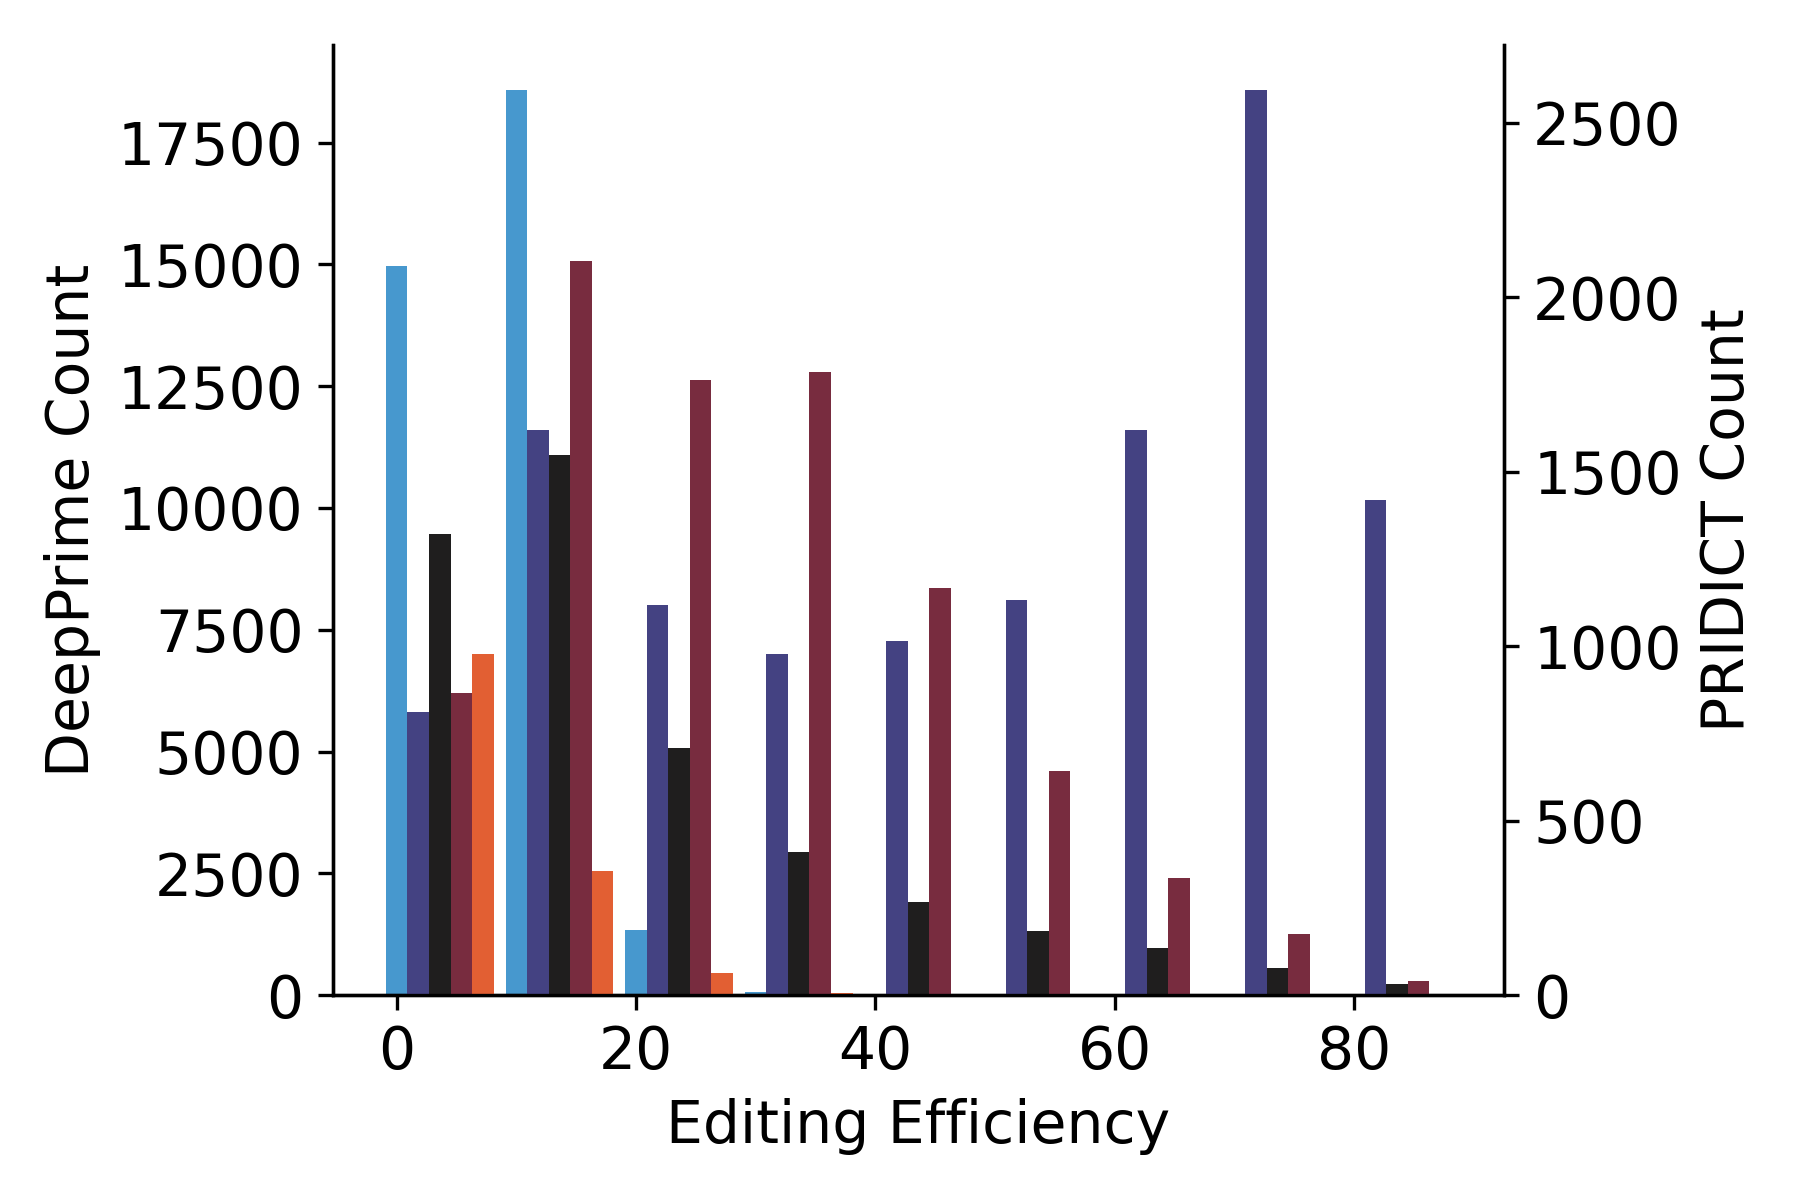
\includegraphics[width=0.45\textwidth]{editing-efficiency-undersample.png}
    }
    \subfigure[Quantile transformation]{
        \label{fig:imbalanced-quantile}
        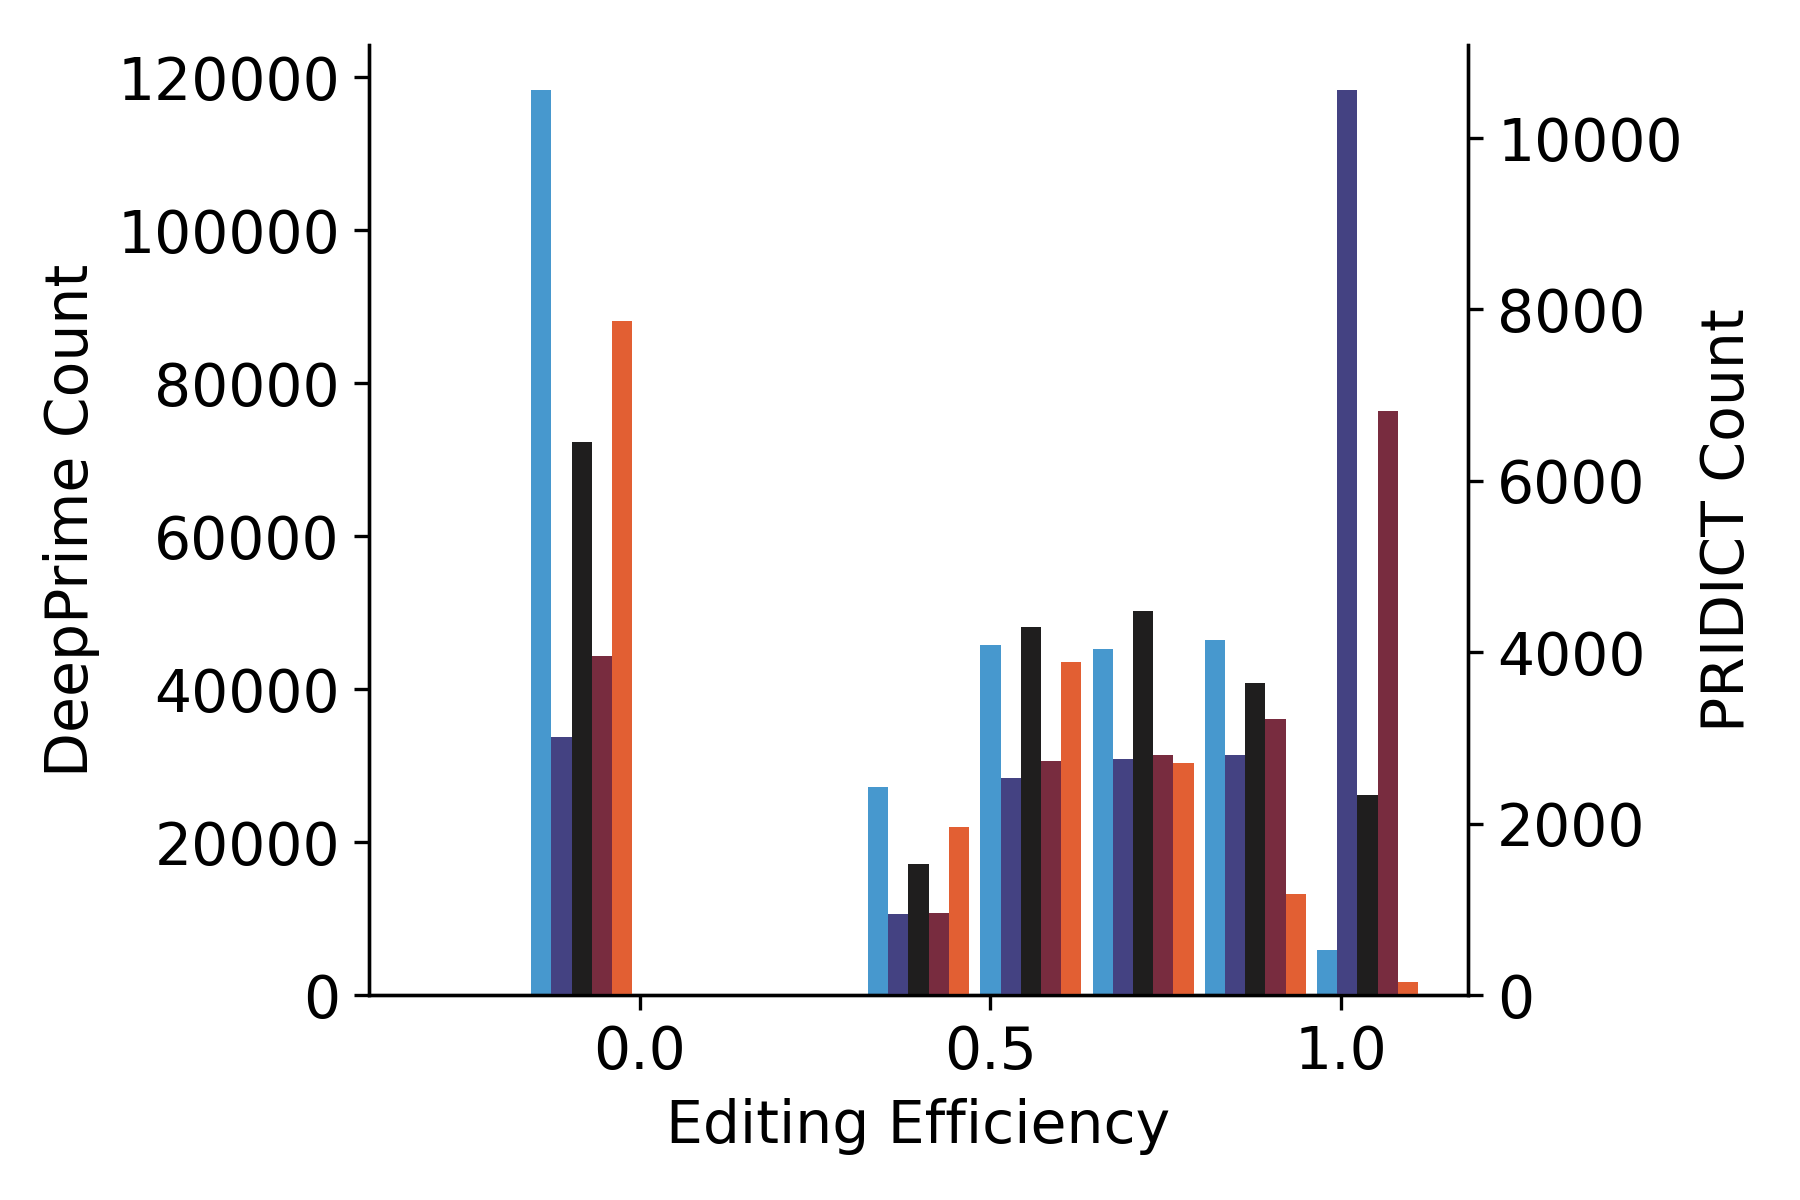
\includegraphics[width=0.45\textwidth]{editing-efficiency-quantile-transform.png}
    }
    \label{fig:imbalanced}
    \caption[Target Distribution Imbalance]{The distribution of the editing efficiency in the DeepPrime HEK293T PE2 (DP) dataset, the PRIDICT2.0 HEK293T (PD HEK293T) dataset, the PRIDICT2.0 K562 (PD K562) as well as K562 MMR deficient (PD K562MLH1DN) dataset, and the PRIDICT2.0 Adv (PD ADV) dataset. (a), followed by the distribution after several adjustments (b-d). Due to the significant different in dataset sizes, DeepPrime datasets and PRIDICT datasets used different y-axis scale (left and right for DeepPrime and PRIDICT respectively): 
    \textbf{(a)} the distribution of original editing efficiency in the datasets. editing efficiency on the x axis is limited to [0, 100], with bin size of 10; \textbf{(b)} the distribution of the log adjusted editing efficiency in the DeepPrime HEK293T PE2 dataset; \textbf{(c)} the distribution of the editing efficiency after undersampling the data with editing efficiency $<10$ with a ratio of 10:1 (10\% of the original data were preserved); \textbf{(d)}, the distribution of the editing efficiency after uniformly quantile transformed.}
\end{figure}

Although the research for imbalanced regression task is relatively limited compared to classification, a number of methods have been proposed\cite{krawczykLearningImbalancedData2016}. The simplest method is to adjust the target values so that better balance can be achived in the projected space. Log transformation is a suitable method for the editing efficiency dataset, as it increases the distance between the lower values while keeping the higher values close (Figure \ref{fig:imbalanced-log}). The numpy \verb|log1p| function was used to prevent the transformation from being undefined when the target value is 0. During inference, the predicted values were transformed back to the original scale using the \verb|expm1| function. Undersampling is also a useful technique, by removing the majority of the lower efficiency pegRNAs, the model can be trained to better predict the higher efficiency pegRNAs. The undersampling ratio was set to 10:1, with the majority of the pegRNAs with efficiency $<10$ removed (Figure \ref{fig:imbalanced-undersampling})\cite{torgoResamplingStrategiesRegression2015}. SMOTE (Synthetic Minority Over-sampling Technique) was also considered, but the generation of synthetic data is very difficult for the prime editing prediction task, as the pegRNA sequence is highly structured and the synthetic data generated may not be biologically feasible. Additionally, quantile transformation was also tested. However, since it discretizes the data, some precision is expected to be lost during the inverse transformation.

In addition to adjusting the dataset itself, the loss function can also be adjusted to assign different importance to different target values. Sample weights can be used to penalize the model more for mispredicting the higher efficiency pegRNAs. 


DeepPrime applied a weighted loss function of the editing efficiency tuned for their dataset:
\begin{equation}
    \text{weight} = \text{min}(\exp(6(\log(x+1)-3)+1),5)
\end{equation}
where x is the measured editing efficiency. The weight is then used in the loss function to penalize the model more for mispredicting the higher efficiency pegRNAs.

At the mean time, PRIDICT did not report any special treatment for the imbalanced dataset, possibly because the having high accuracy for the lower efficiency pegRNAs is as important as predicting the performance higher efficiency pegRNAs accuractely. 

To verify if the adjustments had made any significant different on the model's performance, a simple two layer MLP with 128 hidden units in each layer was trained on the DeepPrime HEK293T PE2 dataset using the original, log adjusted, undersampled and quantile transformed datasets. An additional model using the DeepPrime adjusted MSE was also tested. The models were trained using the Adam optimizer with a learning rate of 0.005, and the learning rate was adjusted using the CosineAnnealingLRWarmRestart scheduler, with a T\_0 (epoch of the first restart) of 15 and T\_mult (the factor to extend the restart intervals) of 1 to escape local minima. 

\begin{figure}
    \centering
    \vspace{-3mm} % Reduce vertical space between subfigures
    \subfigure[DP HEK293T]{
        \centering
        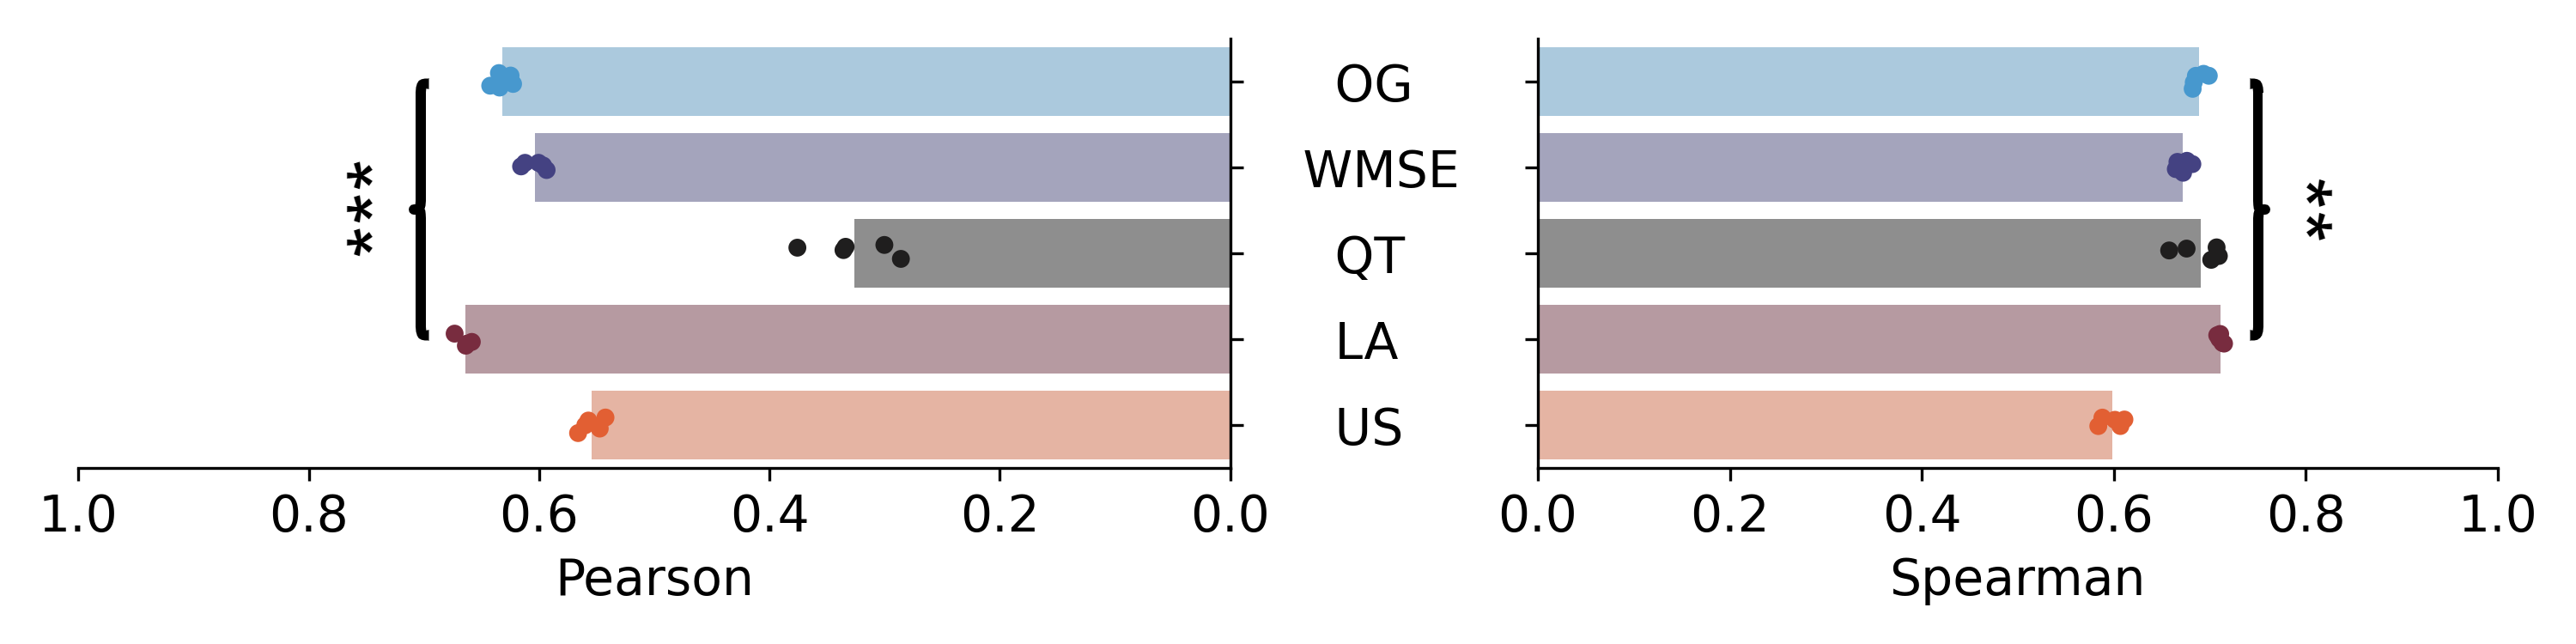
\includegraphics[width=0.8\textwidth]{adjustment-dp-hek293t-performance.png}
        \label{fig:dp-hek293t-adjustment-performance}
    }
    \vspace{-3mm}
    \subfigure[PD HEK293T]{
        \centering
        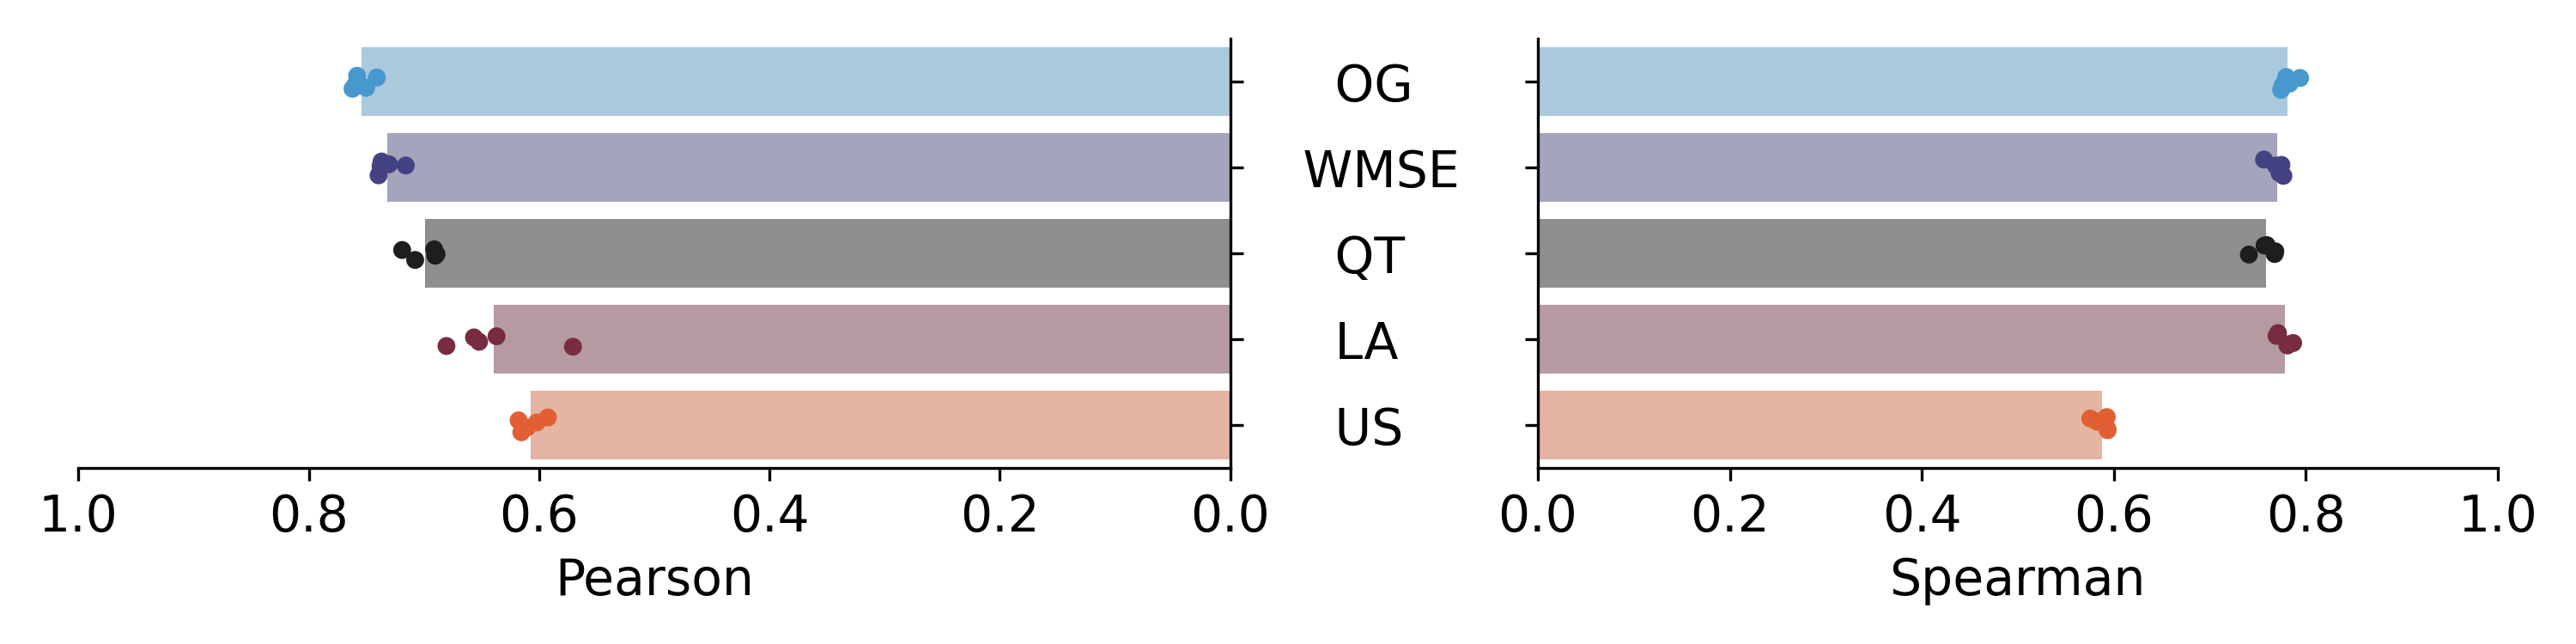
\includegraphics[width=0.8\textwidth]{adjustment-pd-hek293t-performance.png}
        \label{fig:pd-hek293t-adjustment-performance}
    }
    \vspace{-3mm}
    \subfigure[PD K562]{
        \centering
        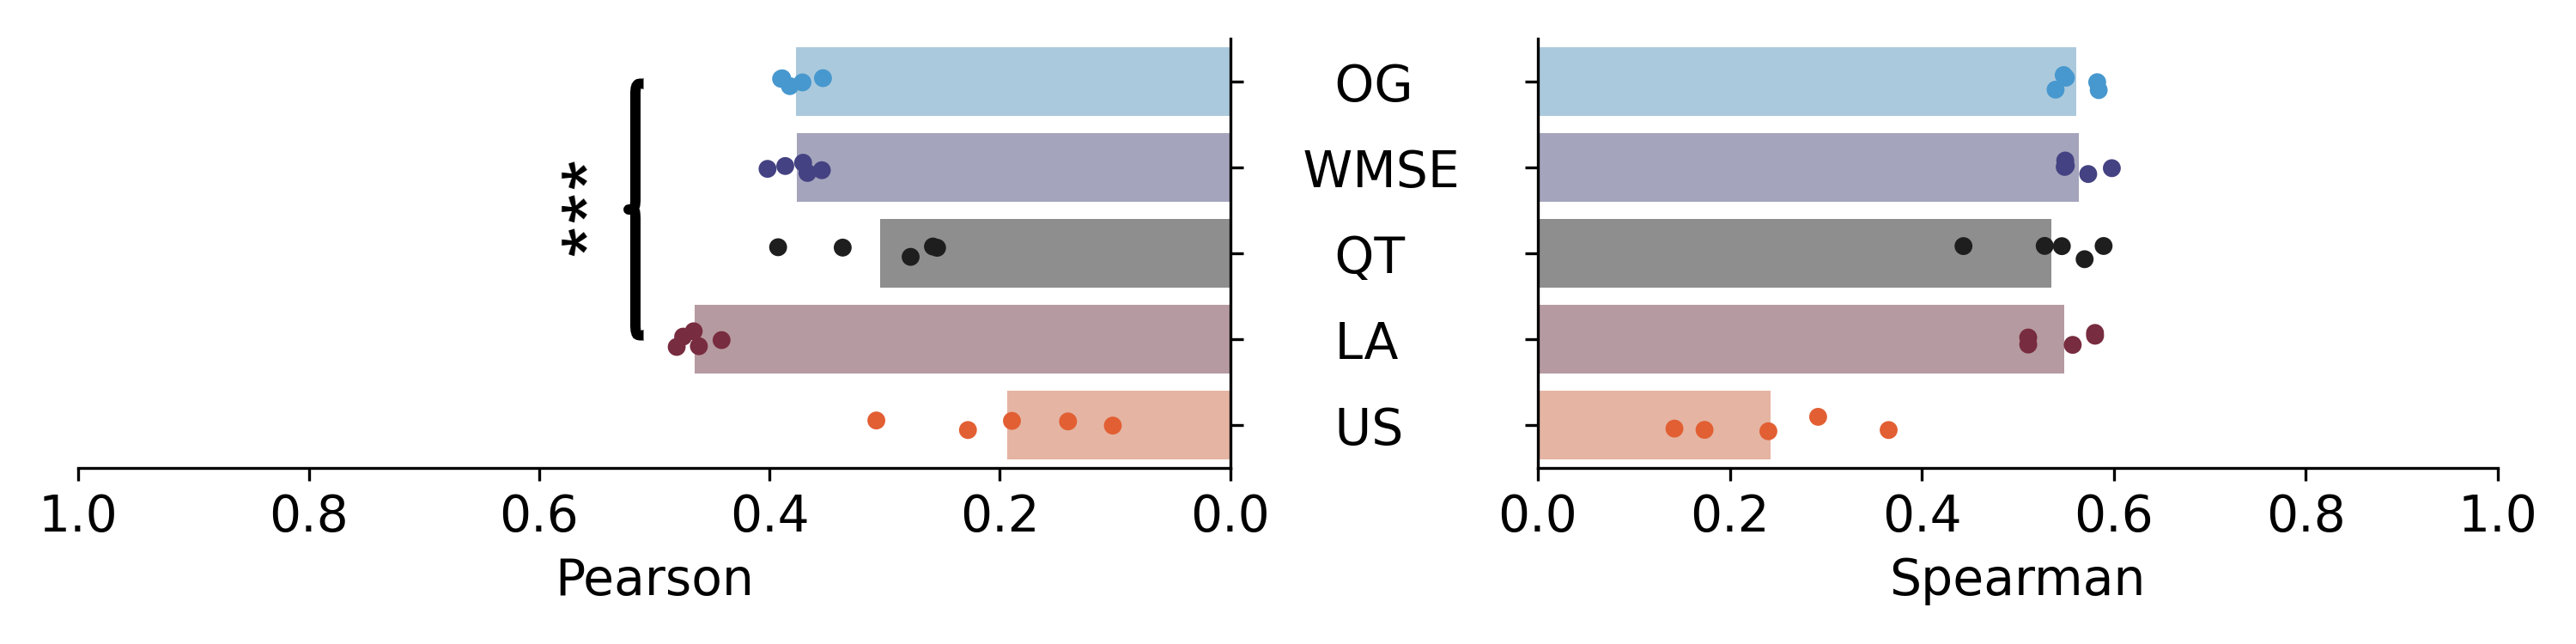
\includegraphics[width=0.8\textwidth]{adjustment-pd-k562-performance.png}
        \label{fig:pd-k562-adjustment-performance}
    }
    \vspace{-3mm}
    \subfigure[PD K562MLH1dn]{
        \centering
        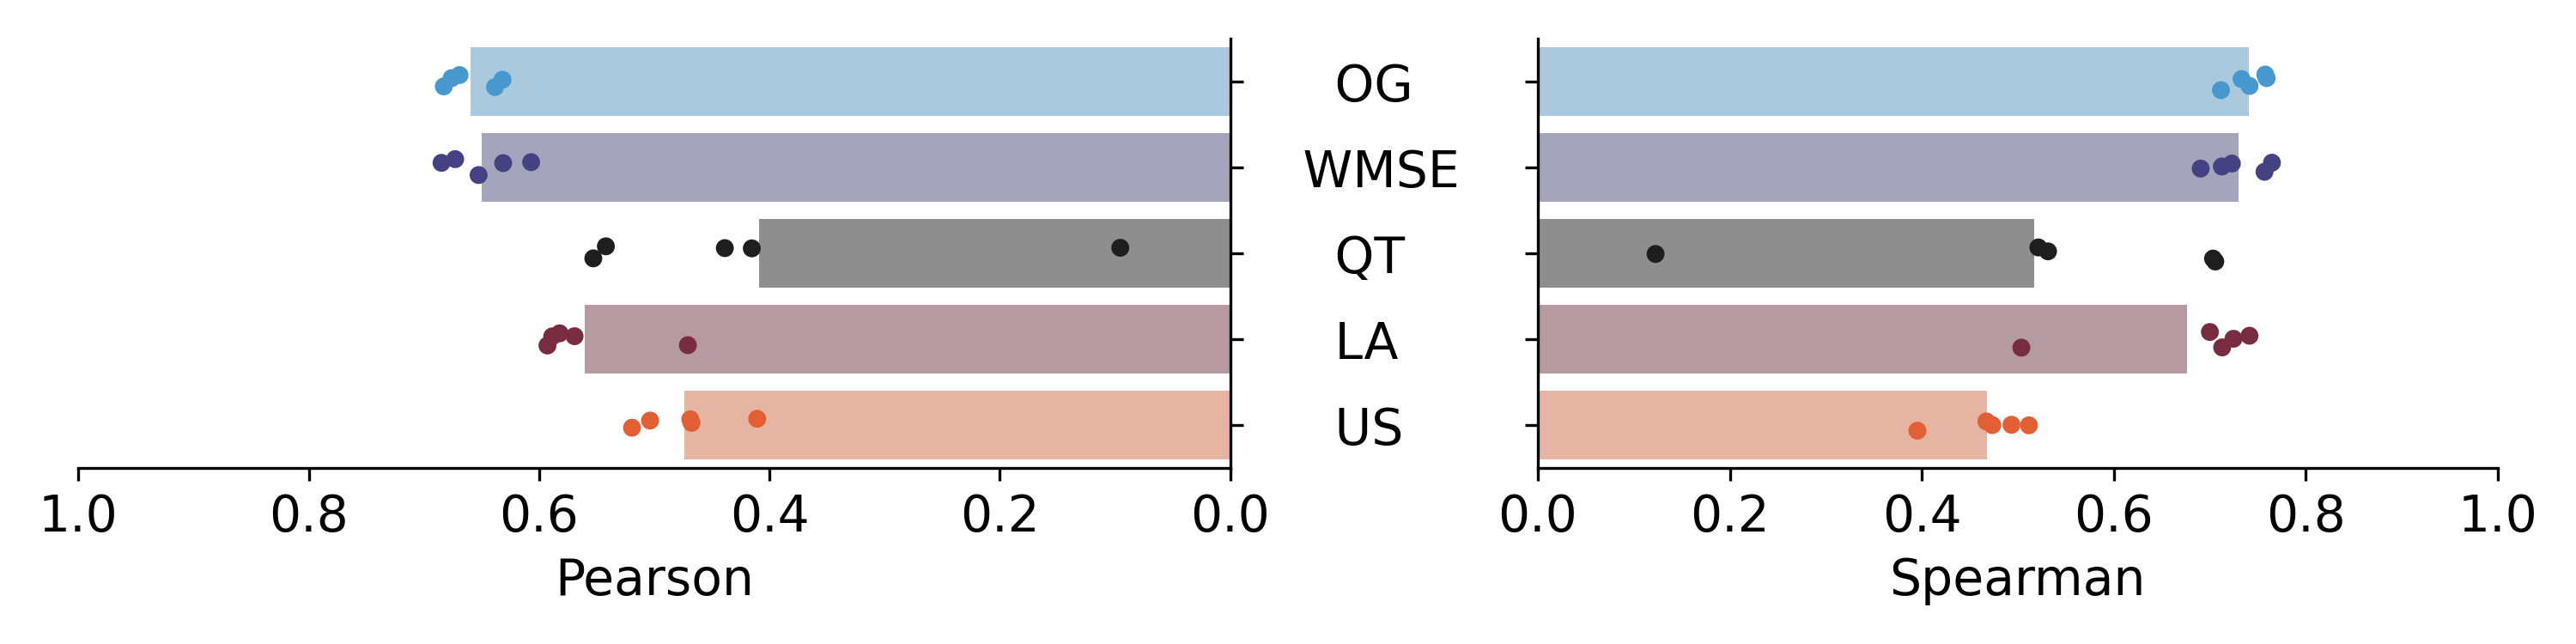
\includegraphics[width=0.8\textwidth]{adjustment-pd-k562mlh1d-performance.png}
        \label{fig:pd-k562mlh1d-adjustment-performance}
    }
    \vspace{-3mm}
    \subfigure[PD Adv]{
        \centering
        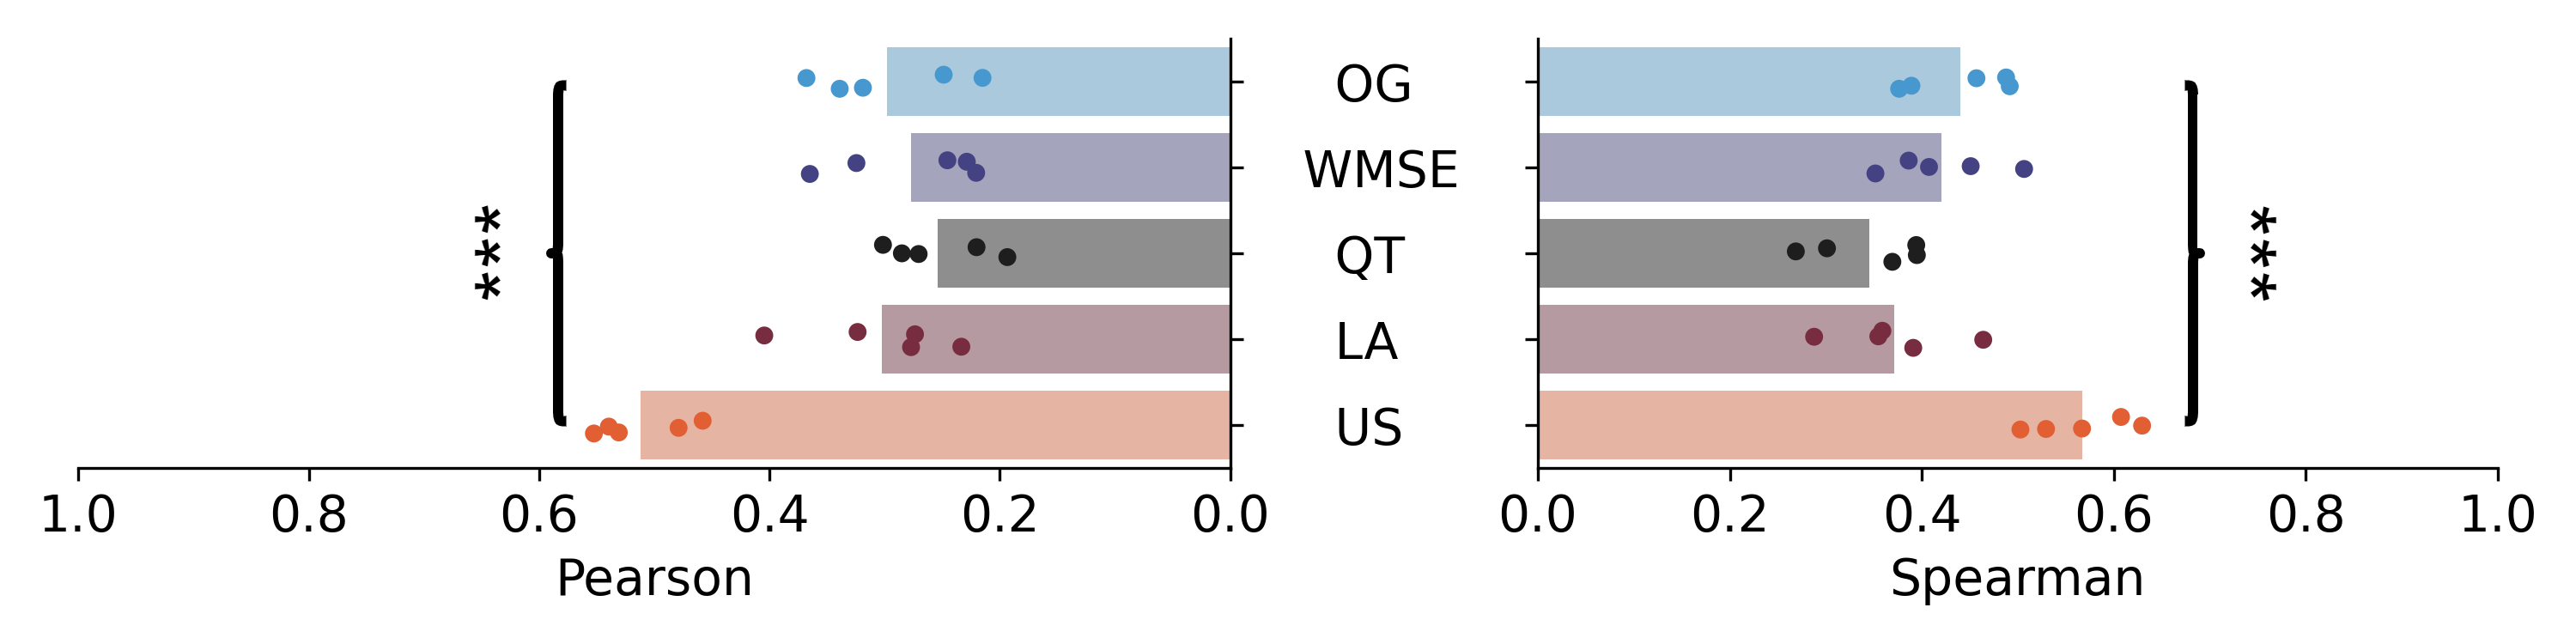
\includegraphics[width=0.8\textwidth]{adjustment-pd-adv-performance.png}
        \label{fig:pd-adv-adjustment-performance}
    }
    \caption{Performance comparison of the MLP model trained on the DeepPrime HEK293T PE2 dataset \textbf{(a)}, the PRIDICT2.0 HEK293T dataset \textbf{(b)}, the PRIDICT2.0 K562 dataset (PD K562\textbf{(c)}), the PRIDICT2.0 K562MLH1d dataset \textbf{(d)}, and the PRIDICT2.0 Adv dataset \textbf{(e)} using the log adjusted (LA), undersampled (US), quantile transformed (QT), and DeepPrime weighted MSE (WMSE) adjustments, in addition to the original dataset and citerion (OG). 
    The performance of each fold is shown as a strip plot on top of the matching bar.}
    \label{fig:adjustment-performance}
\end{figure}

The result of the five adjustments on the five datasets are shown in \autoref{fig:adjustment-performance}. Significant improvements were only observed in three occasions ($p<0.05$, paired t-test between performance in each fold). The log adjustment improved both the Pearson ($p<0.001$) and Spearman ($p<0.01$) correlation of the model on the DeepPrime HEK293T PE2 dataset, as well as the Pearson correlation on the PRIDICT K562 dataset ($p<0.001$), while undersampling noticebly improved both correlation coefficients on the PRIDICT Adv dataset ($p<0.001$). However, the improvement is not universal, as siginificantly lower performance for undersampling was observed on all datasets other than PRIDICT Adv ($p<0.001$). At the same time, log adjustment resulted in severly reduced performance PRIDICT HEK293T and K562MLH1dn datasets ($p<0.001$). 

This narrows down the option to log adjustment and undersampling. numpy provides a very efficienct implementation of the log1p and expm1 functions, making the log adjustment a very attractive option. Meanwhile, the undersampling method is even simpler to implement, and it has the added benefit of reducing the training time, as the model would have to process less data. However, on more complex models, the undersampling method significantly reduce the training size, which may lead to overfitting and reduced validation performance.

% reduce subfigure vertical space
\begin{figure}
    \centering
    \vspace{-3mm} % Reduce vertical space between subfigures
    \subfigure[DP HEK293T]{
        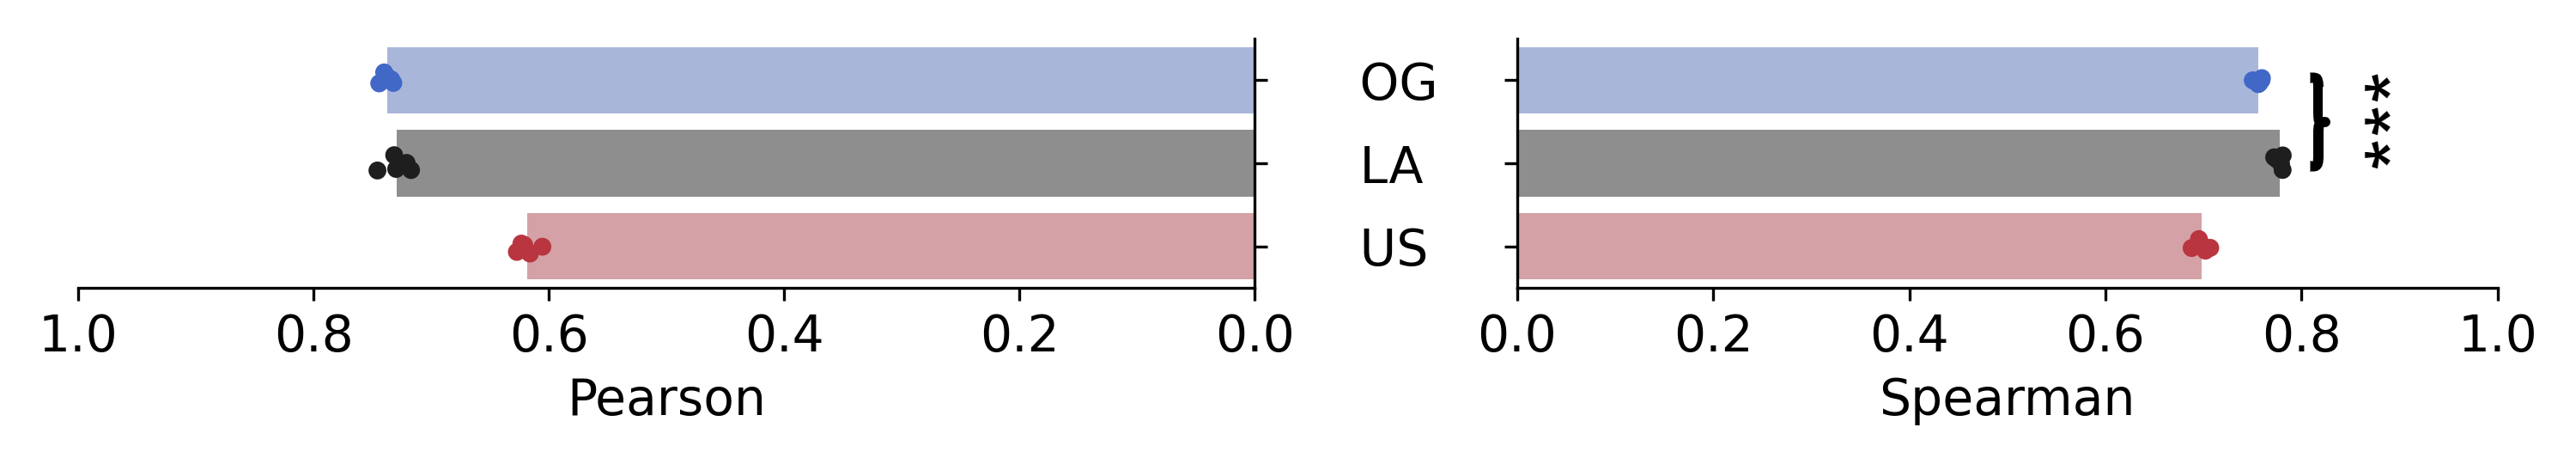
\includegraphics[width=0.8\textwidth]{adjustment-deepprime-dp-hek293t-performance.png}
        \label{fig:deepprime-dp-hek293t-adjustment-performance}
    }
    \vspace{-3mm} % Reduce vertical space between subfigures
    \subfigure[PD HEK293T]{
        \centering
        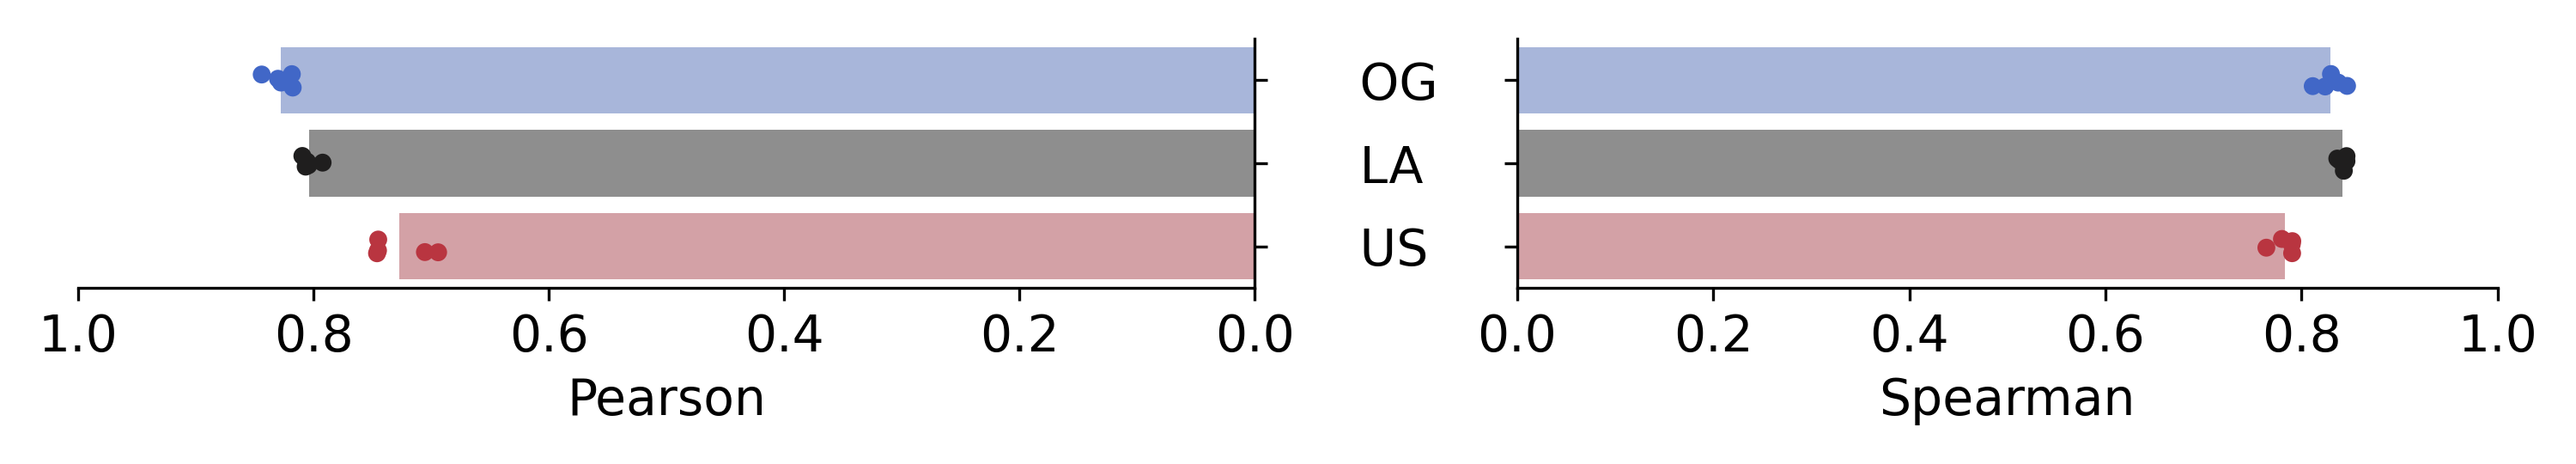
\includegraphics[width=0.8\textwidth]{adjustment-deepprime-pd-hek293t-performance.png}
        \label{fig:deepprime-pd-hek293t-adjustment-performance}
    }
    \vspace{-3mm} 
    \subfigure[PD K562]{
        \centering
        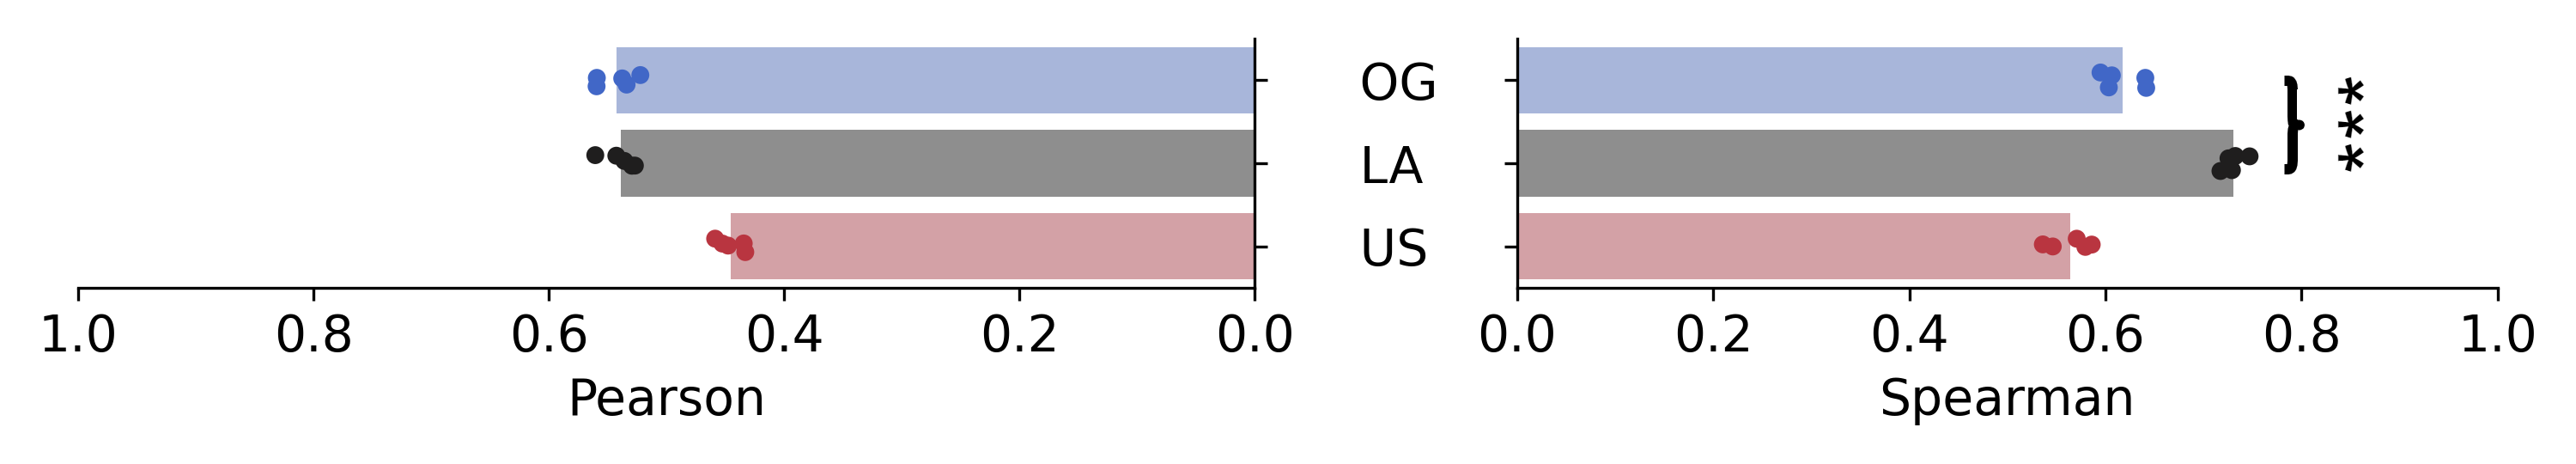
\includegraphics[width=0.8\textwidth]{adjustment-deepprime-pd-k562-performance.png}
        \label{fig:deepprime-pd-k562-adjustment-performance}
    }
    \vspace{-3mm} 
    \subfigure[PD K562MLH1dn]{
        \centering
        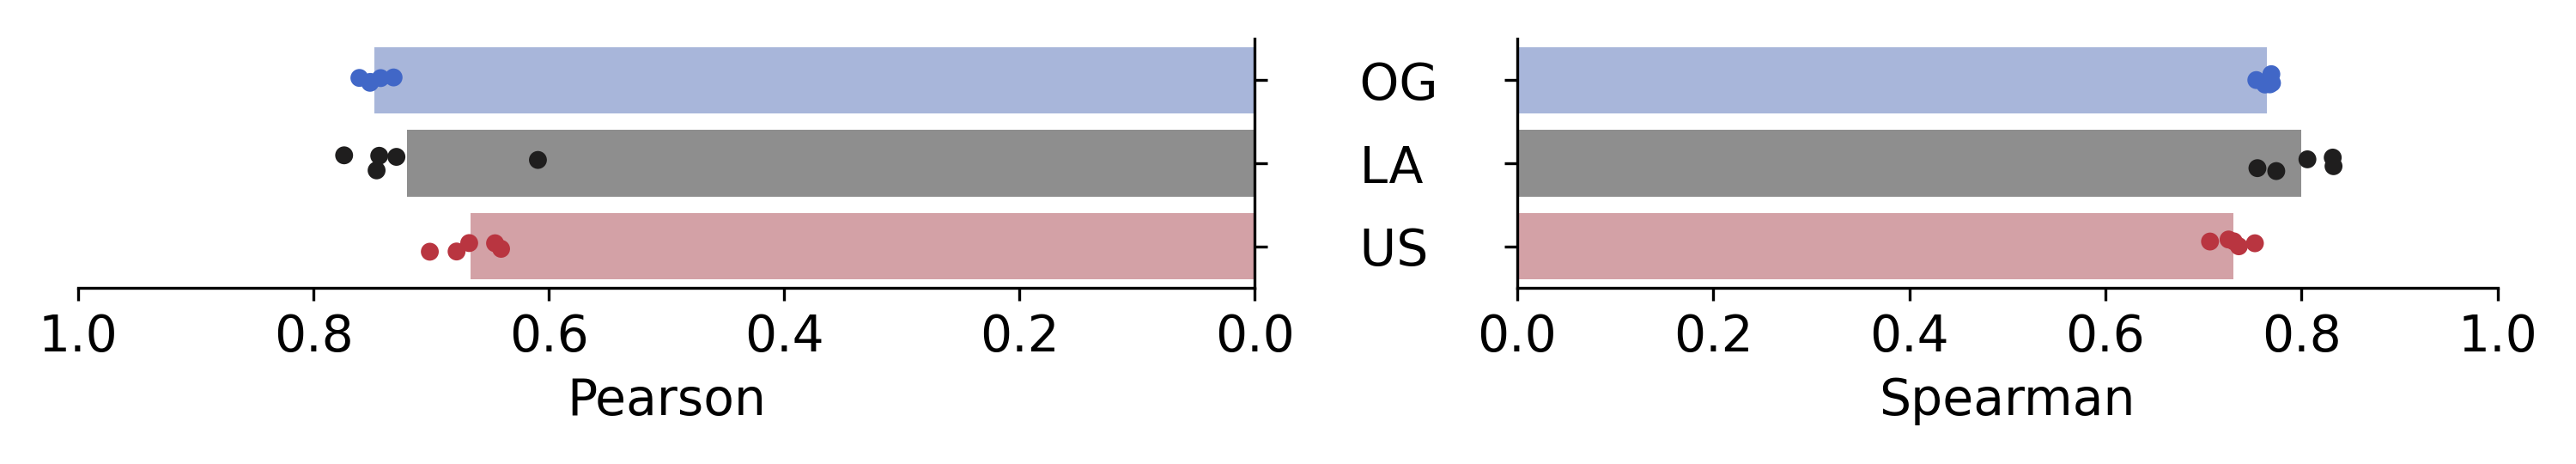
\includegraphics[width=0.8\textwidth]{adjustment-deepprime-pd-k562mlh1d-performance.png}
        \label{fig:deepprime-pd-k562mlh1d-adjustment-performance}
    }
    \vspace{-3mm} 
    \subfigure[PD Adv]{
        \centering
        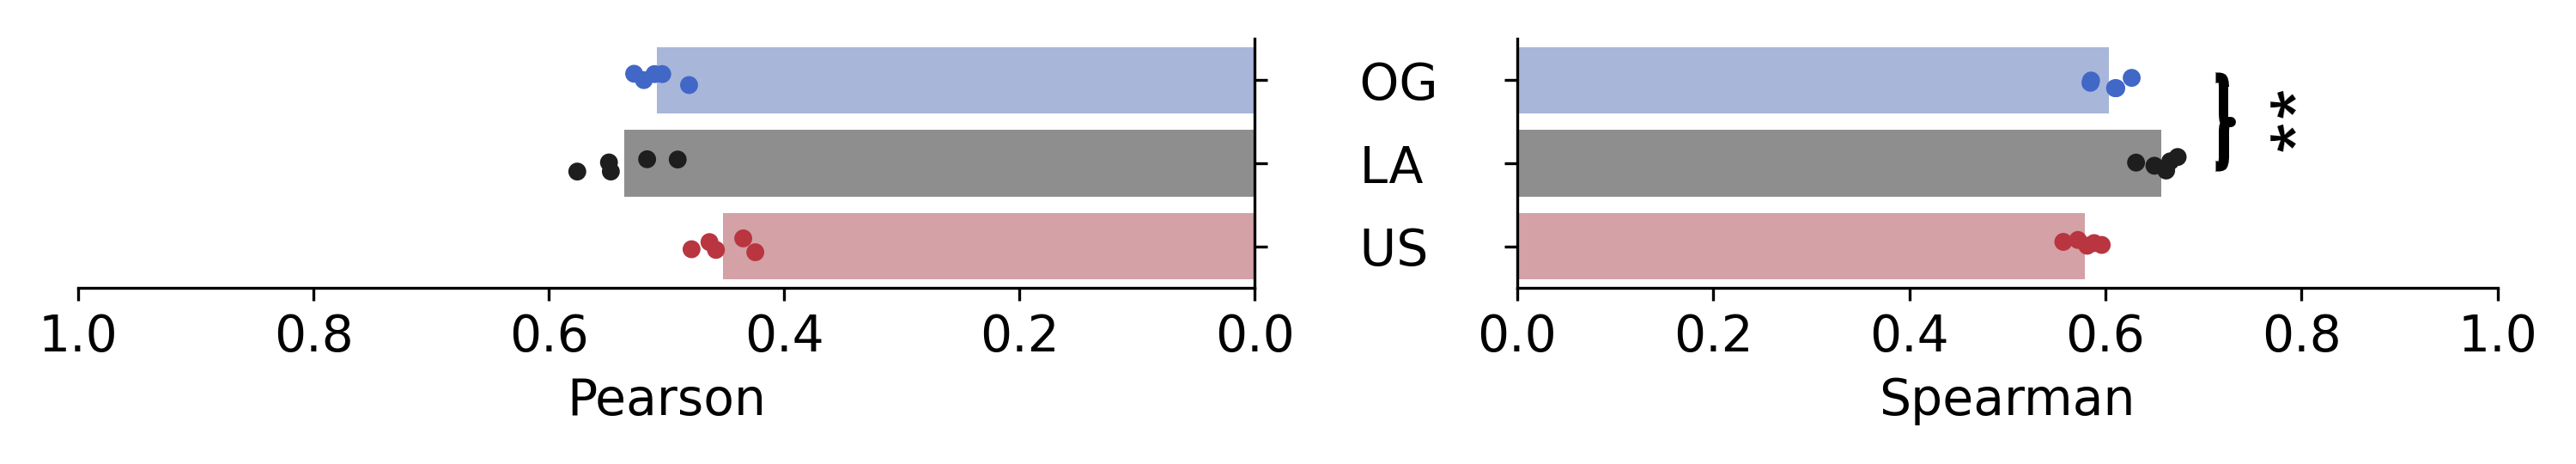
\includegraphics[width=0.8\textwidth]{adjustment-deepprime-pd-adv-performance.png}
        \label{fig:deepprime-pd-adv-adjustment-performance}
    }
    \caption{
        Similar to \autoref{fig:adjustment-performance}, the performance comparison of the MLP model trained on the DeepPrime HEK293T PE2 dataset \textbf{(a)}, the PRIDICT2.0 HEK293T dataset \textbf{(b)}, the PRIDICT2.0 K562 dataset \textbf{(c)}, the PRIDICT2.0 K562MLH1d dataset \textbf{(d)}, and the PRIDICT2.0 Adv dataset \textbf{(e)} using the log adjusted (LA), undersampled (US), and the original dataset (OG). 
    }
    \label{fig:deepprime-adjustment-performance}
\end{figure}

To further verify the necessity of the adjustments, the DeepPrime model with log adjusted and undersampled target were trained on the five datasets using the optimized hyperparameters reported by Yu et al in their study\cite{yuPredictionEfficienciesDiverse2023}. The performance of the models were then evaluated using Pearson and Spearman correlation and compared to the result trained on the original model, shown in \autoref{fig:deepprime-adjustment-performance}.

As expected the relative performance of the undersampling adjustment took a nosedive when training the DeepPrime model with far more parameters than the simple MLP model. Siginificantly lower performance was observed on all datasets ($p<0.01$) trained with undersampled training data. The log adjustment, on the other hand, showed a significant improvement in terms of Spearman's $\rho$ on the DeepPrime HEK293T dataset ($p<0.001$), the PRIDICT K562 dataset ($p<0.001$), and the PRIDICT Adv dataset ($p<0.01$). Additionally, no siginificant decrease in performance was observed other than the DeepPrime and PRIDICT HEK293T datasets ($p<0.05$).

\section{Conventional Machine Learning Models}

Using the top 24 computed features, a number of conventional machine learning models were trained to serve as a baseline for the deep learning models. The models include Lasso and Ridge regression, Random Forest Regressor, Gradient Boosted Trees from the XGBoost library, and a Multi-Layer Perceptron. 

Their hyperparameter were optimized on one fold of the DeepPrime HEK293T using sklearn GridSearchCV. The performance of the optimized models were then evaluated using Pearson and Spearman correlation on the DeepPrime and PRIDICT dataset for three different cell types on all 5 folds to provide a more accurate estimation of the models' performance. The MLP model involved the additional Skorch library to allow for the use of scikit-learn's GridSearchCV for hyperparameter optimization on the Pytorch model. The optimized parameters for the models are as follows:

\begin{itemize}[itemsep=-0mm]
    \item \textcolor{blue}{Lasso}: \verb|alpha=0006158482110660266| (coefficient for penalty term for L1 regularization)
    \item \textcolor{blue}{Ridge}: \verb|alpha=494.17133613238286| (coefficient for penalty term for L2 regularization)
    \item \textcolor{blue}{Random Forest}: \verb|n_estimators=200| (number of trees to build), \verb|max_depth=20| (maximum depth of the trees)
    \item \textcolor{blue}{XGBoost}: \verb|n_estimators=200| (number of boosting rounds, similar to number of trees), \verb|max_depth=5| 
    \item \textcolor{blue}{MLP}: \verb|hidden_layer_sizes=(64, 64)| (two hidden layer with 64 units each), \verb|activation='relu'| (rectified linear unit activation), \verb|solver='adam'| (adaptive moment estimation solver), \verb|lr=0.001| (learning rate)
\end{itemize}

The models' performance were evaluated using Pearson and Spearman correlation between predicted and measured efficiency, and the result of the conventional models on the four datasets were shown in \autoref{fig:conventional_ml_models_performance}. The MLP model has the best overall performance, justifying DeepPrime and PRIDICT's choice of MLP to process extracted features, and prompted me to use a similar design. The XGBoost and Scikit-learn Random Forest trail closely behind, while Lasso and Ridge regression have significantly lower performance. Although similar in accuracy, XGBoost's gradient boosted trees have far superiour efficiency compared to the Random Forest model thanks to its GPU support and optimized implementation ($\sim$300 times faster).

\begin{figure}
    \centering
    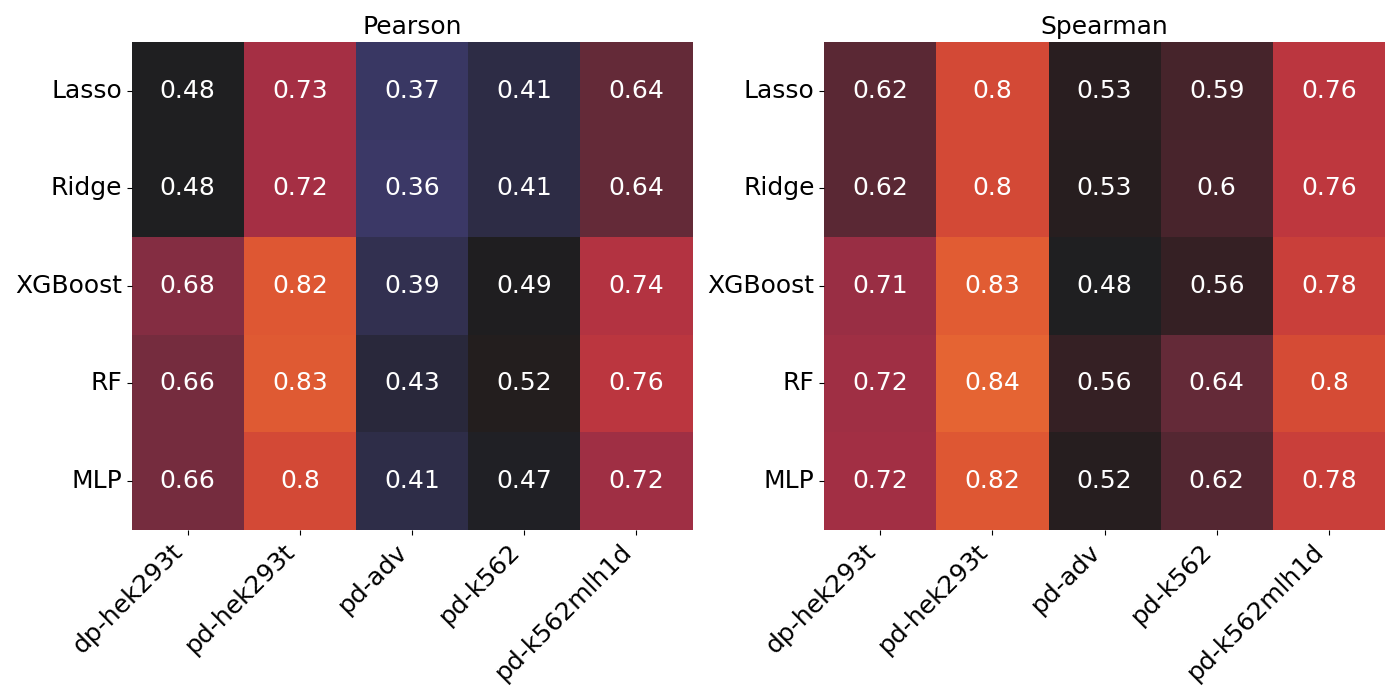
\includegraphics[width=0.8\textwidth]{conventional_ml_models_performance.png}
    \caption[Conventional ML model performance comparison]{Performance compaison in terms of Pearson's r (\textbf{left}) and Spearman's R (\textbf{right}) for a number of conventional machine learning models on the DeepPrime HEK293T PE2 dataset and the PRIDICT2.0 datasets for three different cell lines. The models are Multi-Layer Perceptron(MLP), Random Forest Regressor(RF), Lasso, Ridge, and XGBoost. The performance of the models were evaluated using mean of 5-fold cross validation. The heatmap were mapped to the same scale of [0, 1] for easier comparison.}
    \label{fig:conventional_ml_models_performance}
\end{figure}


\section{Adoption of LLM Method}

The transformer architecture was a ground breaking innovation in the field of NLP, relying solely on self-attention mechanism to create a representation of the input that captures the long range dependencies in the sequences. It was adopted by the Schwank lab (designers of PRIDICT) in the task of base editing efficiency prediction (BE-DICT), and achieved superior performance in multiple datasets compared to its RNN and CNN counterparts\cite{marquartPredictingBaseEditing2021}.

\section{Improving Performance with Ensemble Learning}





For easier identification, the training models stored in `trained-models' directory also follows a uniform naming convention: `model-\{source\}-\{cell-line\}-\{PE-version\}-\{fold\}.pth/pkl/json'. All 5 folds of the models were used during evaluation, and the results were averaged to produce the final prediction. 

Since all of the deep learning models are all effectively an ensemble of a deep learning model and a MLP, XGBoost was chosen to compliment the deep learning models instead of another MLP.

\subsection{Simple Averaging}

\subsection{Stacking}


\subsection{Blending}


\section{Development of pegRNA Design Web Tool}

To facilitate the use of the model in the community, a web tool was developed for users to input their target edit and receive the best pegRNA design as per the model's prediction. The web tool was implemented using the Django framework for easier interaction with Python scripts. 

User input should be in the PRIDICT format of \{at-lesat-100bp\}-(before-edit/after-edit)-\{at-lesat-100bp\}. The user response is then handled by the prediction API endpoint, which would parse the input into original and mutated sequence as well as edit location, type and length. A number of pegRNAs would then be propossed accordingly, and the best performing model would be used to produce an estimation of the editing efficiency for each pegRNA candidate. 

The result is returned as a JSON response and is parsed by the front end as a table of pegRNA candidates with their corresponding editing efficiency. The pegRNA's composition with regard to the wild type sequence can also be visualized by selecting a particular result for easier interpretation.

Other than the model itself, an algorithm for suggesting candidate pegRNAs given a desirable edit was also implemented. Supposing the nick is done at 3bp upstream of the PAM, for the edit to be possible, the PAM sequence must be at most 3bp downstream of the edit start location (in which case LHA length is 0). As discussed in \autoref{sec:determinants}, the length of LHA, RHA and PBS all have significant impact on the editing efficiency. To come up with a recommended range for these parameters, a more detailed analysis of the relationship between the lengths and the editing efficiency was conducted.

\begin{figure}
    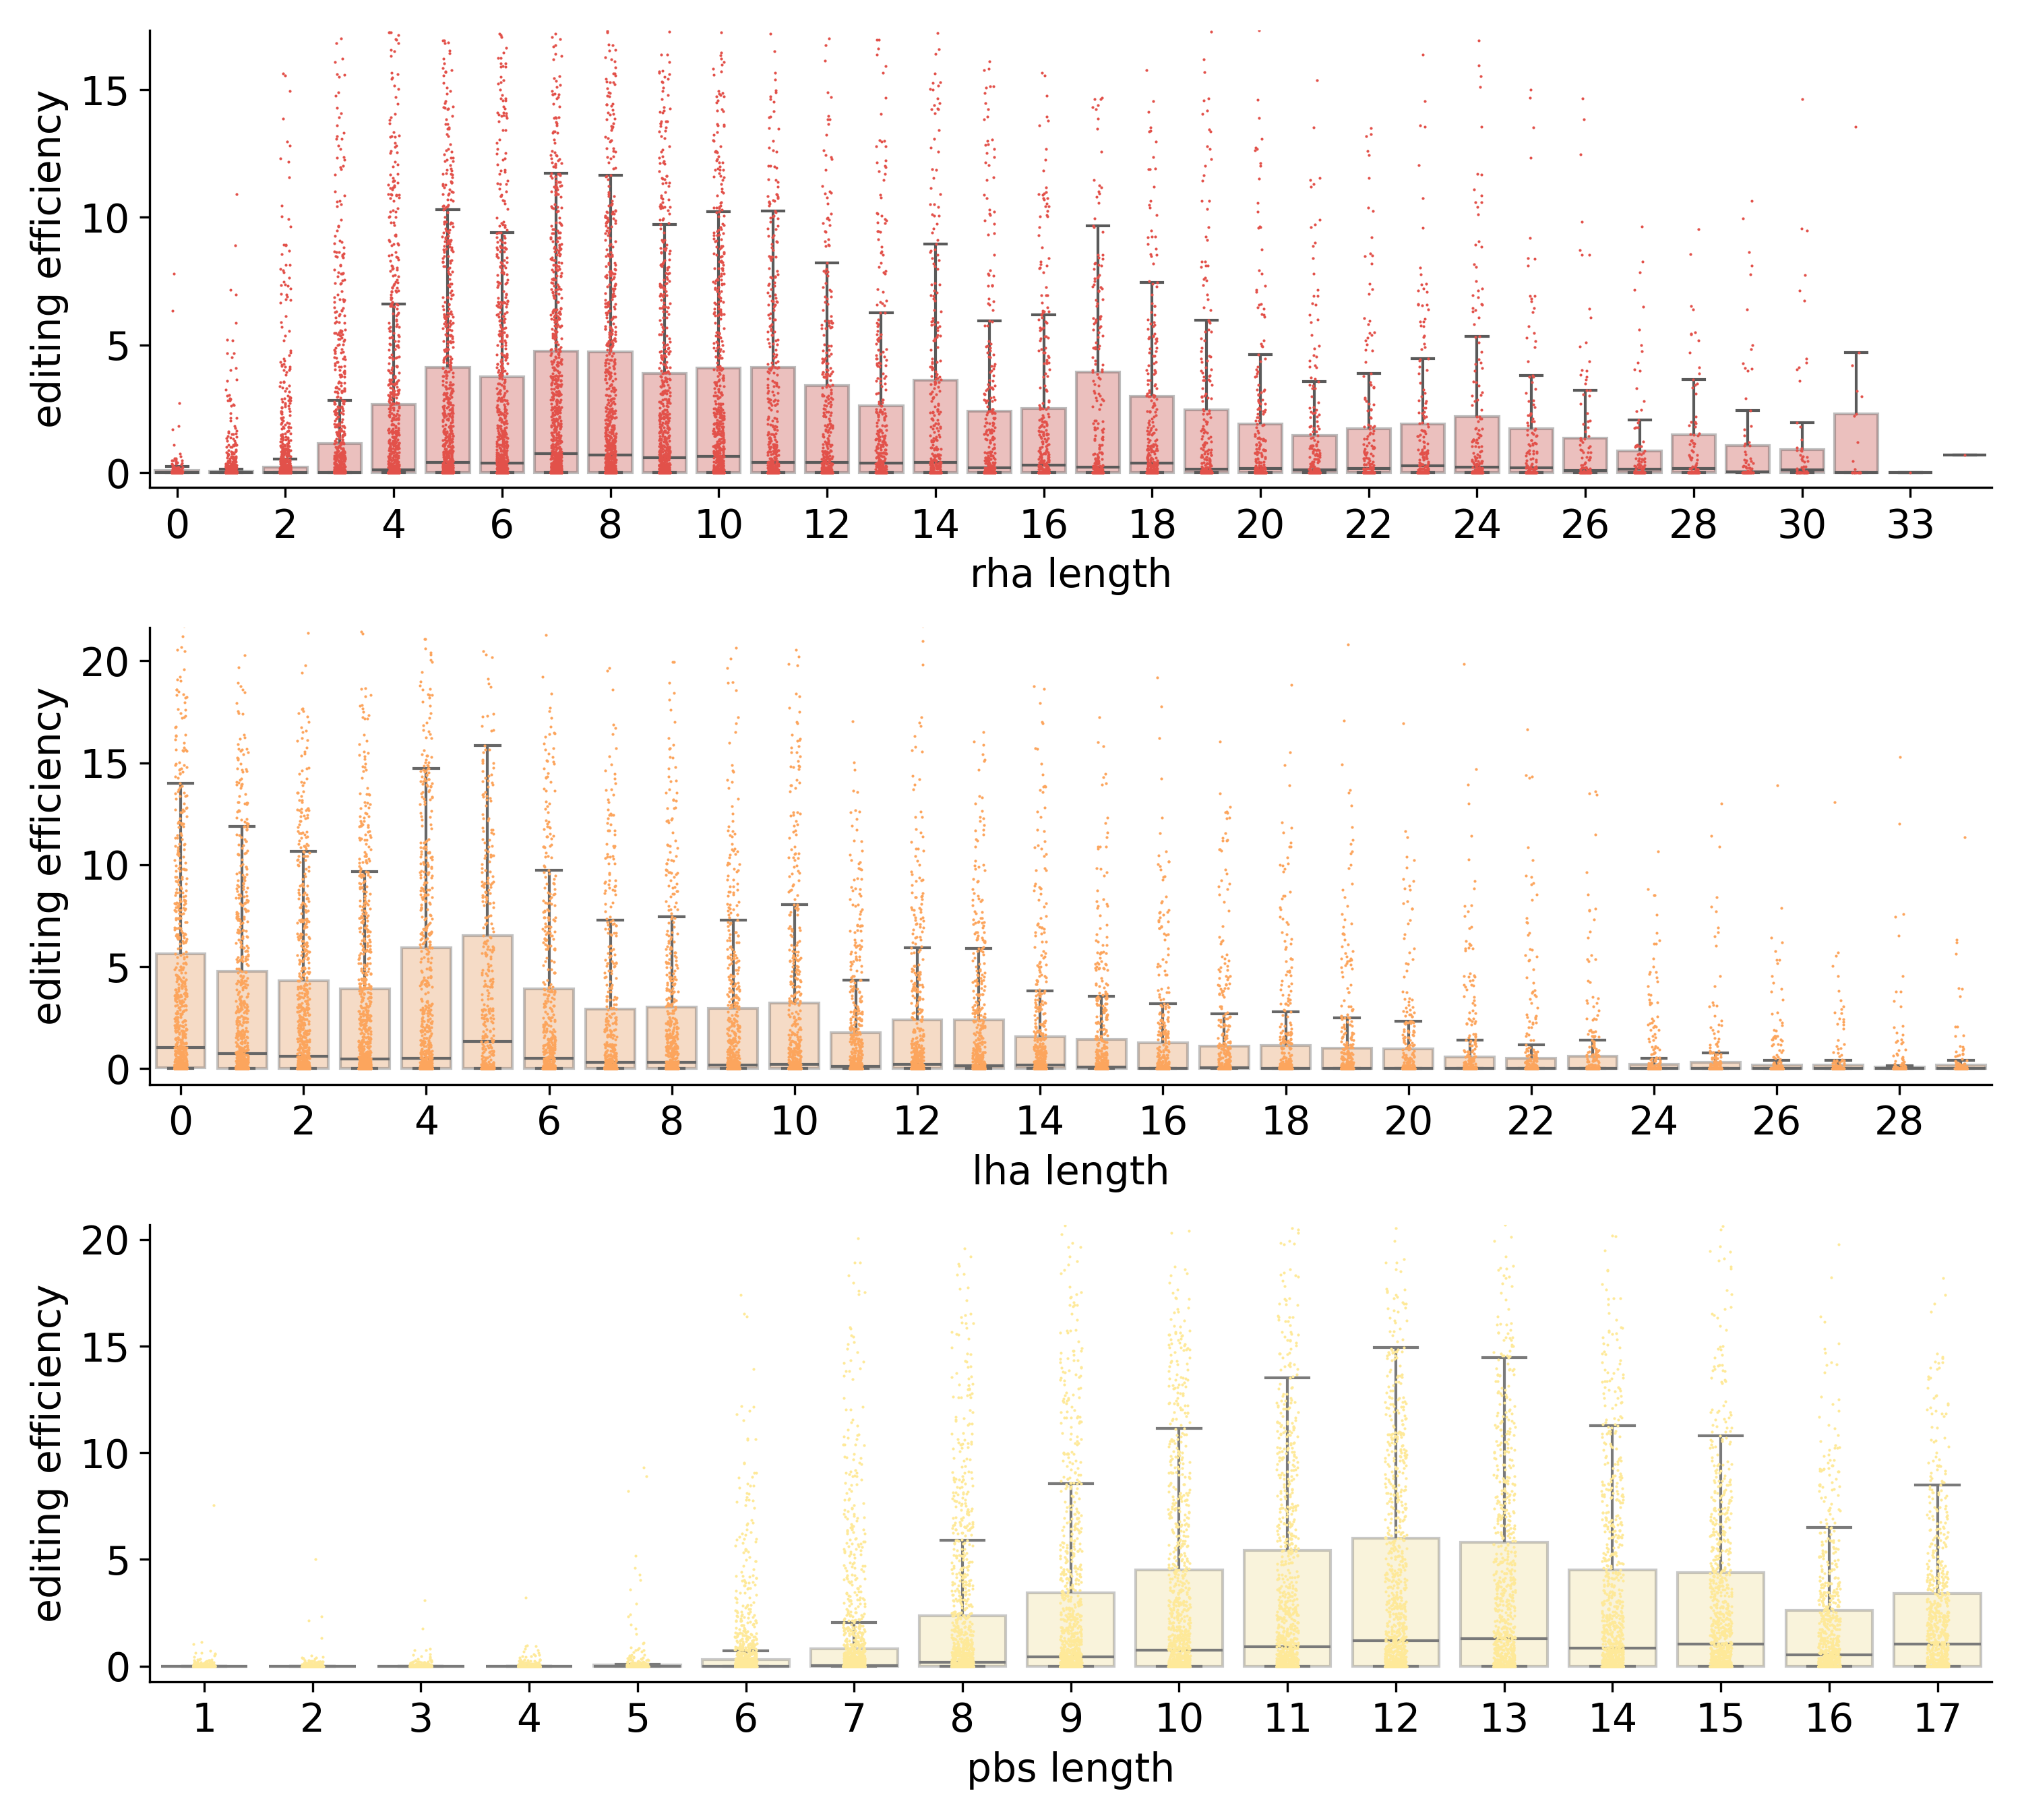
\includegraphics[width=\textwidth]{lha-rha-pbs-length-requirement.png}
    \caption[Relationship between LHA, RHA and PBS length and editing efficiency]{Relationship between PBS (top), RHA (middle) and LHA (bottom) length and editing efficiency. Data from the DeepPrime ClinVar HEK293T PE2 dataset was used in the analysis. random samples of 5\% of the individual data points were plotted as a strip plot on top of the box plot. Y axis is limited to a max value of 5 + 1.5 * IQR to improve readability.}
    \label{fig:lha-rha-pbs-length}
\end{figure}


Shown in \autoref{fig:lha-rha-pbs-length}, the relationship between the lengths of LHA, RHA and PBS and the editing efficiency was analyzed using the DeepPrime ClinVar HEK293T dataset. Consistent with Yu et al, 2023's finding, editing editing efficiency plateaued with RHA length of 7-12bp. Since RHA is the component with the greatest flexibility in length as it does not depend on target location, I decided to only use the 7-12bp range where the corresponding efficiency is the highest so that the resulting search space can be smaller.  As for LHA, the efficiency was shown to decrease with longer LHA length, with an elbow point at around 20bp, where the decrease significantly slows down. Thus, the recommended distance between the nick and the edit location is set to 0-20bp, and this is only extended if no suitable PAM is found within the range. Last but not least, as expected, PBS length's impact on the editing efficiency is roughly normally distributed, with the highest efficiency at around 12bp. Decent performance can be observed from 8bp all the way up to the highest recorded value of 17bp, which covers the entire range of the protospacer upstream of the nick site. Thus, although the SHAP analysis showed that long PBS can be detrimental to the editing efficiency, the range of PBS length was still set to 8-17bp.

In summary, unless specified otherwise by the users, the algorithm would only propose pegRNAs with component length in the range specified in \autoref{tab:recommended-range}.

\begin{table}[h]
    \centering
    \begin{tabular}{c|c|c}
        % \hline
        \textbf{Component} & \textbf{Min Length} & \textbf{Max Length} \\
        \hline
        LHA & 0 & 20 \\
        RHA & 7 & 12 \\
        PBS & 8 & 17 \\
        % \hline
    \end{tabular}
    \caption{Recommended range for LHA, RHA and PBS length}
    \label{tab:recommended-range}
\end{table}


Limited by the scale and funding of this project, the web tool was not deployed to a public server, but instead packaged in a container for local use with Docker. 

It is also accessible using Python with Django and Pytorch installed by executing 

\verb|python webtool/manage.py runserver|

suppose that the user is in the root directory of the project. The web tool can then be accessed by visiting \verb|http://127.0.0.1:8000/|.
\chapter{Benchmarking and Result}

\section{Fine Tuning the Deep Learning Models}

On top of the five main dataset of size $> 20k$, DeepPrime has additional 18 datasets of size $\sim5k$, which were used to fine tune the model for better generalizability. As a result, for a more thorough comparison between the models, the same fine tuning process was conducted on all deep learning models.

To fine tune the models, the same hyperparameters during the original training were used, except for the learning rate, which was lowered to $1e-3$ for the fine tuning to accommodate the smaller dataset size. Additionally, the NRCH versions of prime editors were used in some of the small datasets, which contains optimized SpCas9 proteins that can accommodate NRCH PAMs (N = A, T, C, G; R = A, G; H = A, C, T) \cite{millerContinuousEvolutionSpCas92020}. The pam matching function was thus updated to accommodate the additional PAMs.

To preserve the sequence features acquired on the DeepPrime main dataset, the sequence processing layers were frozen, leaving only the feature processing and the final meta learner to be trained. The models were trained for at most 300 epochs for each fold, and the best model was selected based on the validation loss.

% TODO: add references to the section and appendix after including the results

\subsection{Performance on All Datasets}

As discussed in \autoref{sec:ensemble}, all three ensemble models were able to significantly outperform the base learners on the PRIDICT HEK293T PE2 dataset. Thus, power weighted mean ensemble, bagging and adaboost were trained on all available datasets alongside the transformer model to evaluate their performance against the base learners, as well as DeepPrime and PRIDICT.

\subsection{Performance on Individual Editing Types}

\section{Attention Analysis}
\label{sec:attention_analysis}

\begin{figure}
    \centering
    \subfigure[Substitution]{
        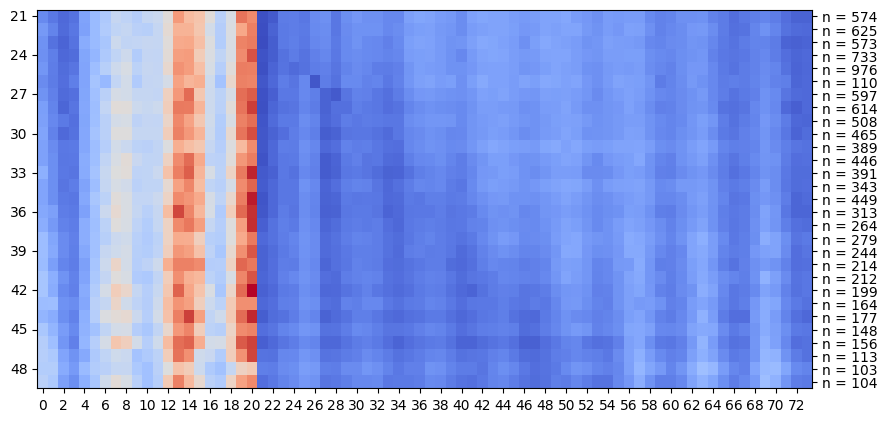
\includegraphics[width=0.88\textwidth]{dp-hek293t-pe2-transformer-only-attention-insertion.png}
        \label{fig:attention_insertion}
    }
    \subfigure[Insertion]{
        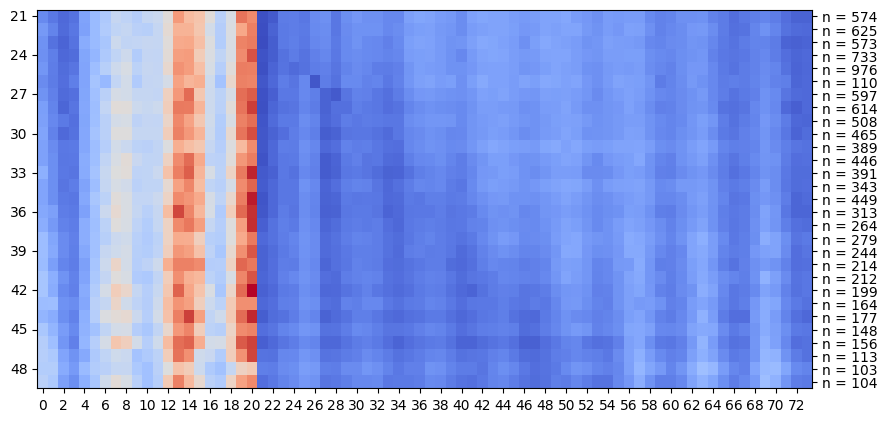
\includegraphics[width=0.88\textwidth]{dp-hek293t-pe2-transformer-only-attention-insertion.png}
        \label{fig:attention_substitution}
    }
    \subfigure[Deletion]{
        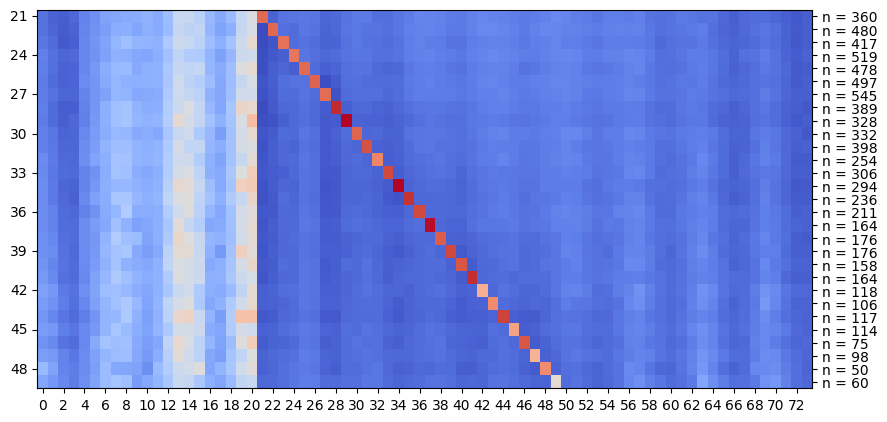
\includegraphics[width=0.88\textwidth]{dp-hek293t-pe2-transformer-only-attention-deletion.png}
        \label{fig:attention_deletion}
    }
    \caption[Attention weights for the DeepPrime model trained on the HEK293T-PE2 dataset]{Attention weights of length 1 edits for the DeepPrime model trained on the HEK293T-PE2 dataset. The x-axis represents the position of the transformer output token, the y-axis indicates the edit position. Red colour indicates higher attention weights, while blue indicates lower attention weights. The example size for each edit location is shown on the right in the format of 'n=number of examples'.}
    \label{fig:attention}
\end{figure}

A significant advantage of the attention based methods are their interpretability. The attention mechanism allows the model to focus on specific parts of the input data using the attention weights, which can be visualized teo understand the model's decision making process. 

In this architecture, the most informative and interpretable attention weights are the feature embedding attention weights at the final layer of the transformer model, pooling all token embeddings into a single feature embedding by attributing different weights to each token position. 

The examples were grouped together by their editing type and length so that the edit positions can be easily identified and compared. And the attention weights for edits at the same position were aggregated to show the overall importance of the position in the editing efficiency prediction.

The model trained on the biggest DeepPrime dataset was first tested, as the transformer model has the greatest chance of learning the underlying motifs influencing the editing efficiency in the data. Starting with the edits of length 1, the attention weights were visualized for the substitution, insertion, and deletion, shown in \autoref{fig:attention}. 

For both 1-bp substitution and insertion, the attention weights were the highest from around the start of the protospacer location (location 4) to the nick position (location 20, also where the PBS ends). This may be an indication that the model considers the composition of the PBS as an important feature for the editing efficiency prediction. Additionally, one of the hot spots for the attention weights was the protospacer location 13 to 17. This is consistent with the finding in \autoref{fig:shap} that the composition of the protospacer is an important feature for the editing efficiency prediction.

However, for deletion, the attention weights were the highest at the edit position. The cross attention output of the edit position for deletion was dominated by the encoder output, as the self-attention weights for the mutated sequence at edit position were masked out to be zero. This is a possible indication that the model considers the base to delete as an important feature for the deletion operation.

\begin{figure}
    \centering
    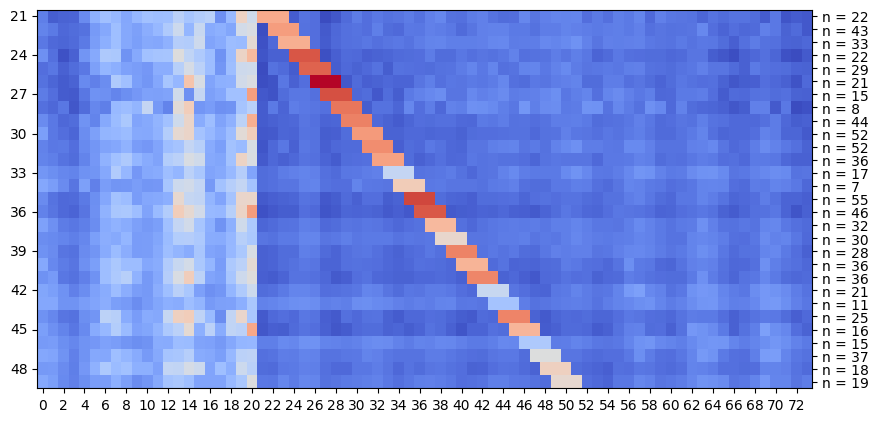
\includegraphics[width=0.9\textwidth]{dp-hek293t-pe2-transformer-only-attention-deletion-3bp.png}
    \caption[Attention weights for 3-bp deletion of the DeepPrime model trained on the HEK293T-PE2 dataset]{Similar to \autoref{fig:attention}, attention weights of length 3 deletion for the DeepPrime model trained on the HEK293T-PE2 dataset.}
    \label{fig:attention_deletion_3bp}
\end{figure}

The attention weights for the edits of length 3 showed similar result (\autoref{fig:attention_deletion_3bp}), the only noticeable difference is that the high attention regions for deletion were extended to 3bp long, reflecting the longer deletion length.

During SHAP analysis in \autoref{sec:determinants}, the edited base was not investigated, as a meaningful representation for bases of different lengths could not be found. Thus, to understand if the base to edit during deletion is indeed an important feature, SHAP analysis was conducted again on the HEK293T PE2 dataset for 1-bp replacement, insertion, and deletion (\autoref{fig:shap-1bp})

\begin{figure}
    \subfigure[Replacement]{
        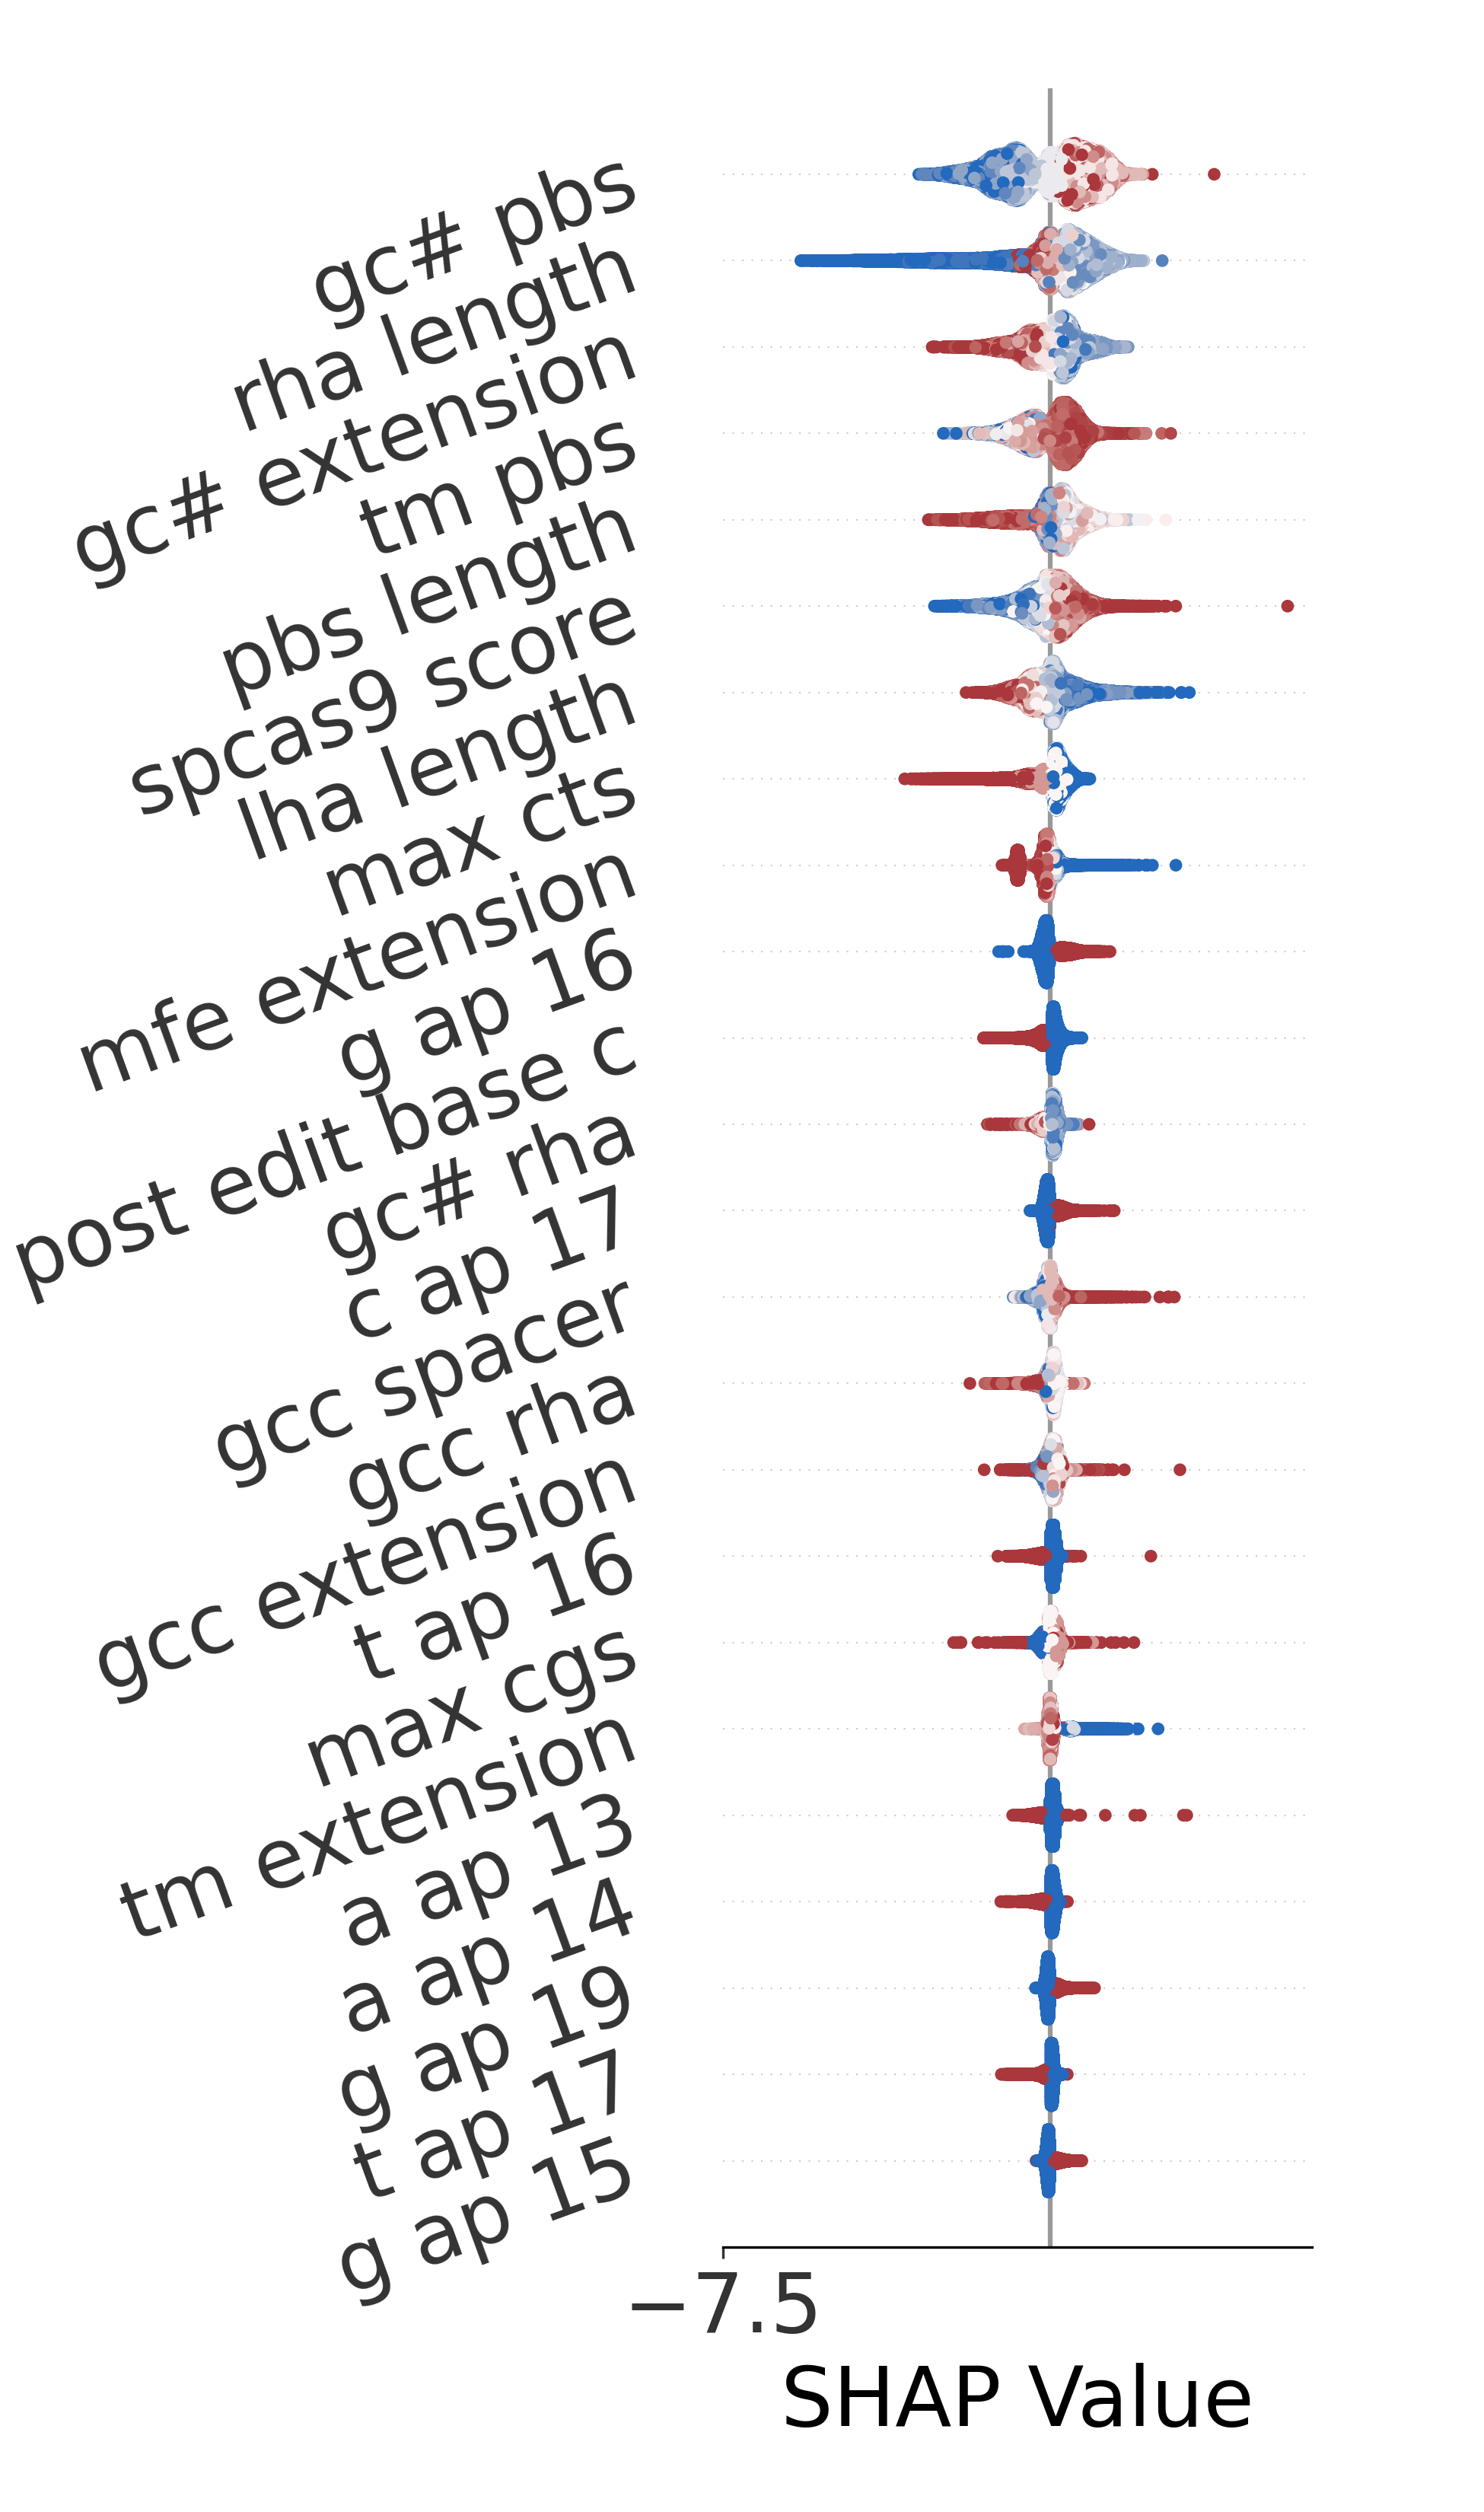
\includegraphics[width=0.33\textwidth]{shap_1bp-dp-hek293t-pe2-replace.png}
        \label{fig:shap_replacement}
    }%
    \subfigure[Insertion]{
        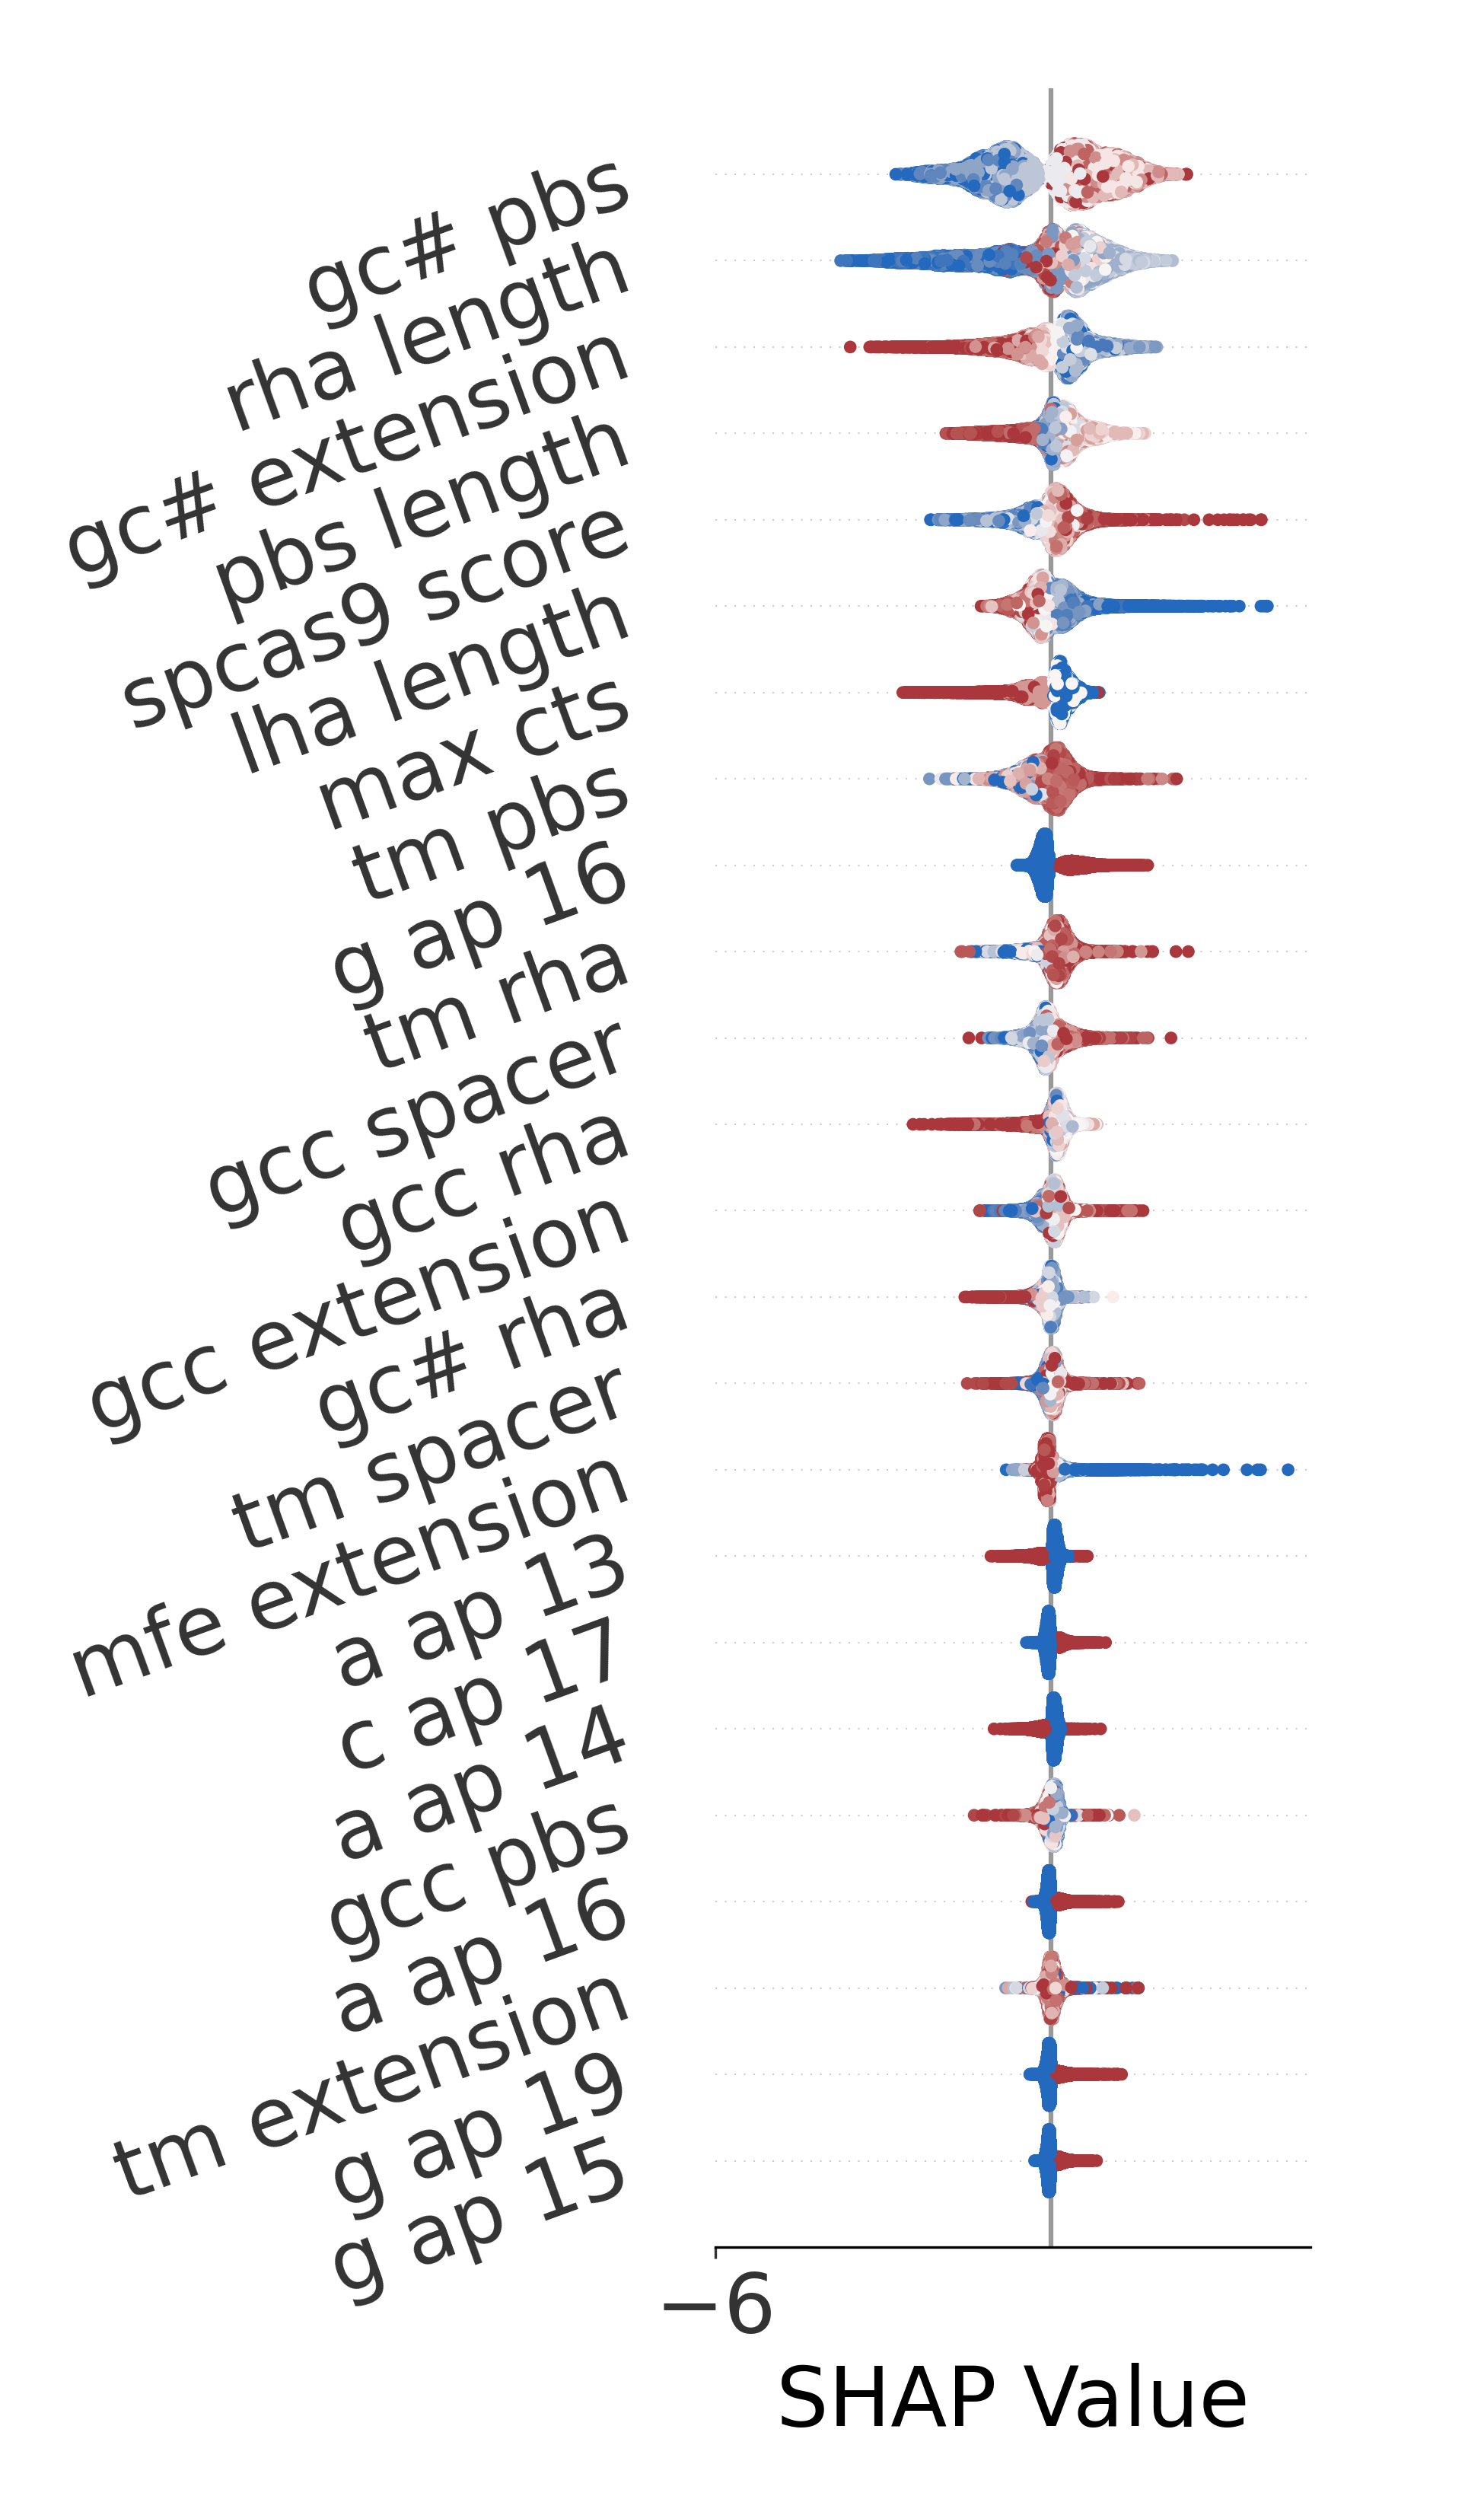
\includegraphics[width=0.33\textwidth]{shap_1bp-dp-hek293t-pe2-insert.png}
        \label{fig:shap_insertion}
    }%
    \subfigure[Deletion]{
        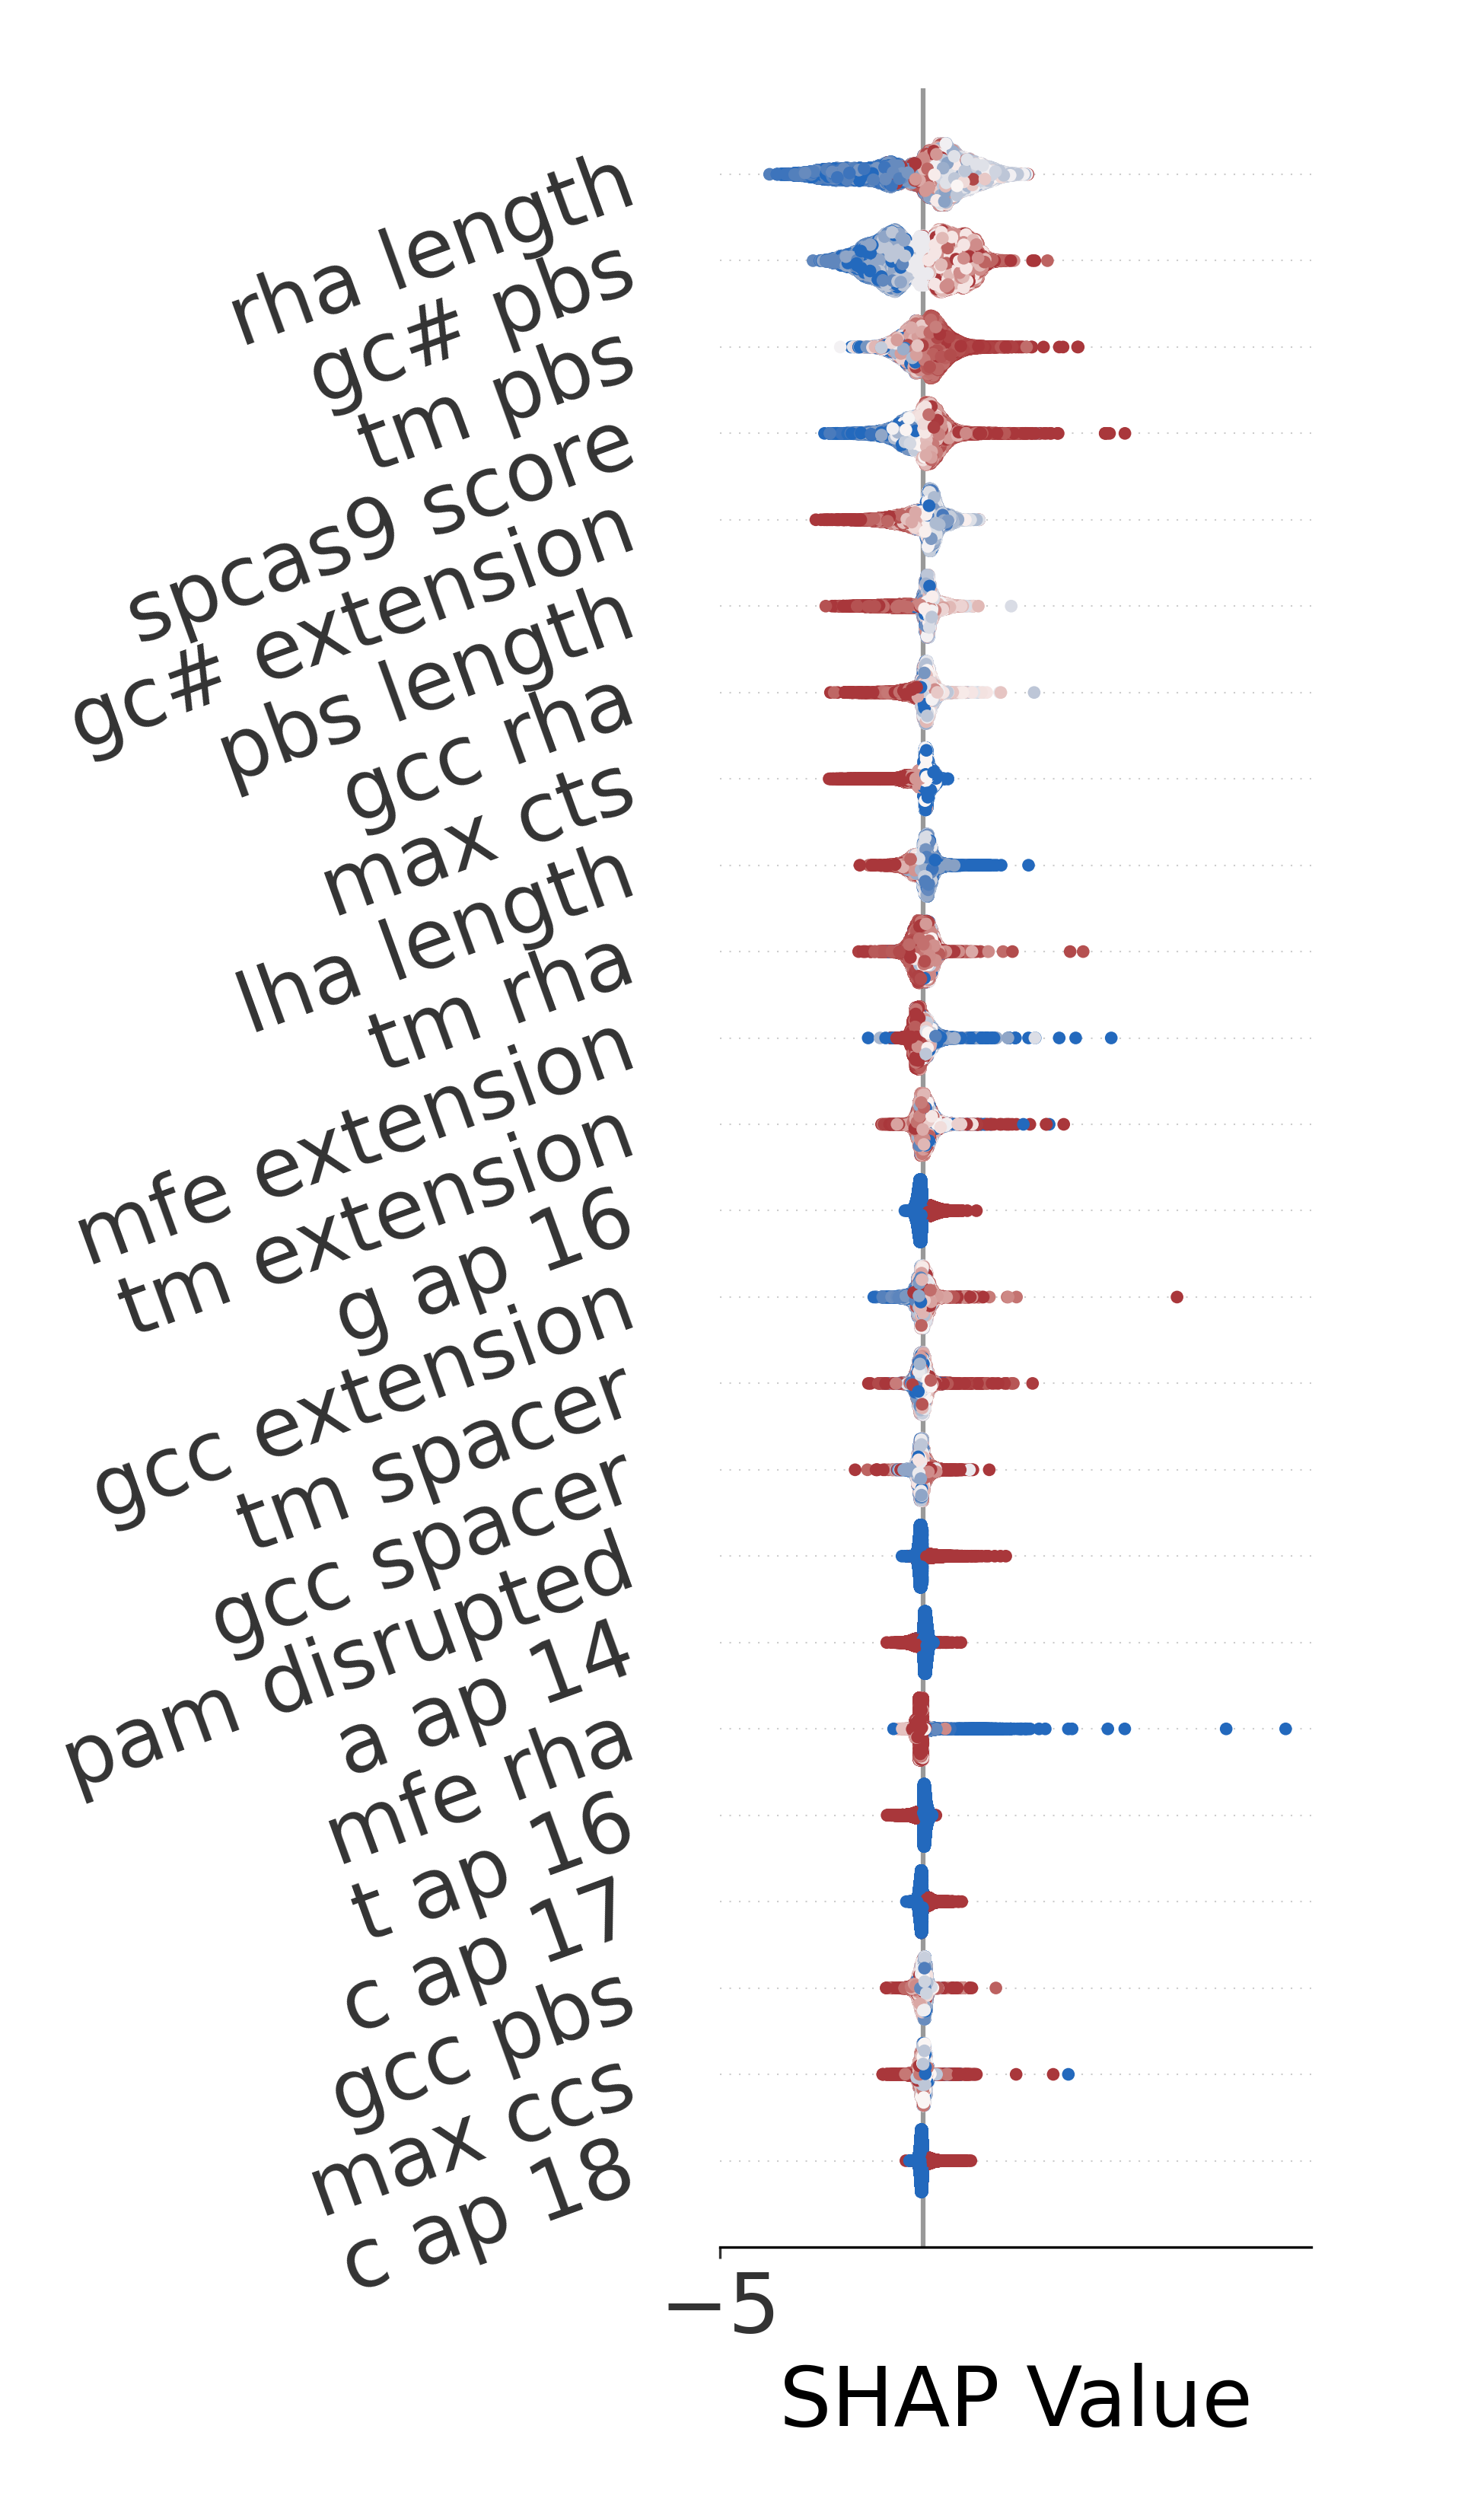
\includegraphics[width=0.33\textwidth]{shap_1bp-dp-hek293t-pe2-delete.png}
        \label{fig:shap_deletion}
    }
    \caption[SHAP analysis for 1-bp insertion and deletion of the DeepPrime model trained on the HEK293T-PE2 dataset]{SHAP analysis for 1-bp insertion and deletion of the DeepPrime model trained on the HEK293T-PE2 dataset. The x-axis represents the attributed weight to the outcome (SHAP value), while the y-axis represents the feature importance. The colour of the points indicates the feature value, with red indicating high values and blue indicating low values.}
    \label{fig:shap-1bp}
\end{figure}

Interestingly, different from the attention weights, the base to edit during deletion was not considered an important feature by the model (Figure \ref{fig:shap_deletion}). 
\chapter{Discussion}

Overall, the ensemble models have shown promising results in predicting the efficiency of prime editing in a number of configurations of prime editors and cell lines. They were able to achieve on par performance with the current state of the art model, PRIDICT and DeepPrime on most datasets other than the DeepPrime HEK293T PE2 dataset. 

Additionally, as discussed in the benchmarking section, the ensemble models may be able to achieve better performance than the current state of the art models on more datasets if they were tuned to the specific dataset instead of using one set of hyperparameters for all datasets. 

However, the transformer model underperformed in this task, unable to achieve the same level of performance as the ensemble models on the five main datasets. This is possibly due to the inherent differences between the tasks of prime editing and base editing efficiency prediction. 

For base editors, the editing window is relatively static with regard to the protospacer location. At the same time, each base editor can only introduce a single type of base change (C to T or A to G) at a single location in the protospacer. This limits the number of possible outcomes for each base editor to a small number of possibilities, and the relationship between the wild type and mutated sequence is relatively predictable.

Meanwhile, the prime editing efficiency prediction task is much more complex. The prime editor can introduce a variety of changes to the target sequence, and the editing window is also dynamic, as the prime editor can introduce changes at different locations after the nick site of the protospacer. This results in a much larger number of possible outcomes, and the attention mechanism might have a much harder time capturing enough features specific to each edit.

A number of possible improvements could be made to the transformer model to help it establish the connection between wild type and mutated sequences. 

On the data preprocessing level, we had established that the functional annotation denoting the PBS and RTT sequences used by PRIDICT was important for the performance of the transformer model. However, the number of possible edits given the locations of the PBS and RTT sequences is still very large. It may be beneficial to incorporate the actual bases of the PBS and RTT sequences into the wild type sequence to help the model establish the connection between the wild type and mutated sequences. 

On top of that, I avoided modifying the architecture of the transformer model too much as the development of a new architecture would require a significant amount of time and resources beyond the limit of this project. However, a number of alternative architectures can be explored that may improve upon the performance of the transformer model.

For example, the transformer model could be modified to include a convolutional neural network (CNN) layer at the input to help the model capture local features in the sequence. At the same time, a number of different generator could be used to generate the output of the transformer model other than the feature embedding attention layer used in this study. A number of possibilities include another CNN layer, a gated recurrent unit used by DeepPrime, or a simple feedforward neural network. 

Finally, as briefly mentioned in \autoref{sec:determinants}, the current methods all follow the same general approach of training one model for each prime editor and cell line combination. However, recent research has shown that multi-task learning can be beneficial in a number of different tasks, including the prediction of the efficiency of base editors\cite{mollaysaAttentionbasedMultitaskLearning2023a}

Obviously, this would introduce many problems during implementation. The most prominent issue would be the assembling of the dataset. As discussed in \autoref{sec:determinants}, many cellular level factors can affect the efficiency of prime editing. These factors were ignored in this study since they were encapsulated in the cell line and prime editor. However, if a single model were to be trained for all prime editors and cell lines, these factors would have to be included in the dataset. This may require substantial biological knowledge and could involve scrapping multiple sequencing datasets to obtain the necessary information. 
More imbalance in the dataset would also arise, for example, cells with MMR deficiency may become underrepresented and cause the model to perform poorly on these cell lines. 
These problems would require significantly more resources (both in time and data) to solve, and should be an interesting topic for future research.


\startappendices
% Add or remove any appendices you'd like here:


%%%%% REFERENCES


{\renewcommand*\MakeUppercase[1]{#1}%

% \chapter{Summary and Comparison of Existing Learning Based Models}

\label{appendix:models}

\section{DeepPE}

Developed by Kim et al, DeepPE is one of the earliest attempt at predicting the outcomes of prime editing using machine learning and illustrated many possible determinants of PE efficiency. Most of the determinants discovered in their study are still valid today, but the model itself is not as relevant in terms of performance due to the constraints in datasets at the time of their publication. The model is also very limited in terms of editing types supported, focusing on predicting the efficiency of G to C substitution at the position +5 nick site of the target sequence. 

After the users provided the target sequence to edit, the web tool will propose a number of pegRNA sequences and evaluate their efficiency using the DeepPE model. The 47-nt long target sequence and the 17 to 37nt RTT+PBS sequences, as well as 20 explicit features including the GC content and melting temperature of the PBS are used as input to the model. The two nucleotide sequences are one-hot encoded into four dimensional matrices. The two embedded sequences and the explicit features are then concatenated(stacked) together and fed into a convolutional neural network with 10 $3 \times 4$ filters. The output is pooled using a deep reinforcement learning model instead of a traditional pooling layer, and then input into a fully connected layer with 1000 units. The result is linearly transformed to the DeepPE prediction score, indicating the efficiency of the editing process on the target sequence using the provided PBS and RTT.

A sketch of the model architecture is shown in \autoref{fig:deeppe}.

\begin{figure}[ht]
    \centering
    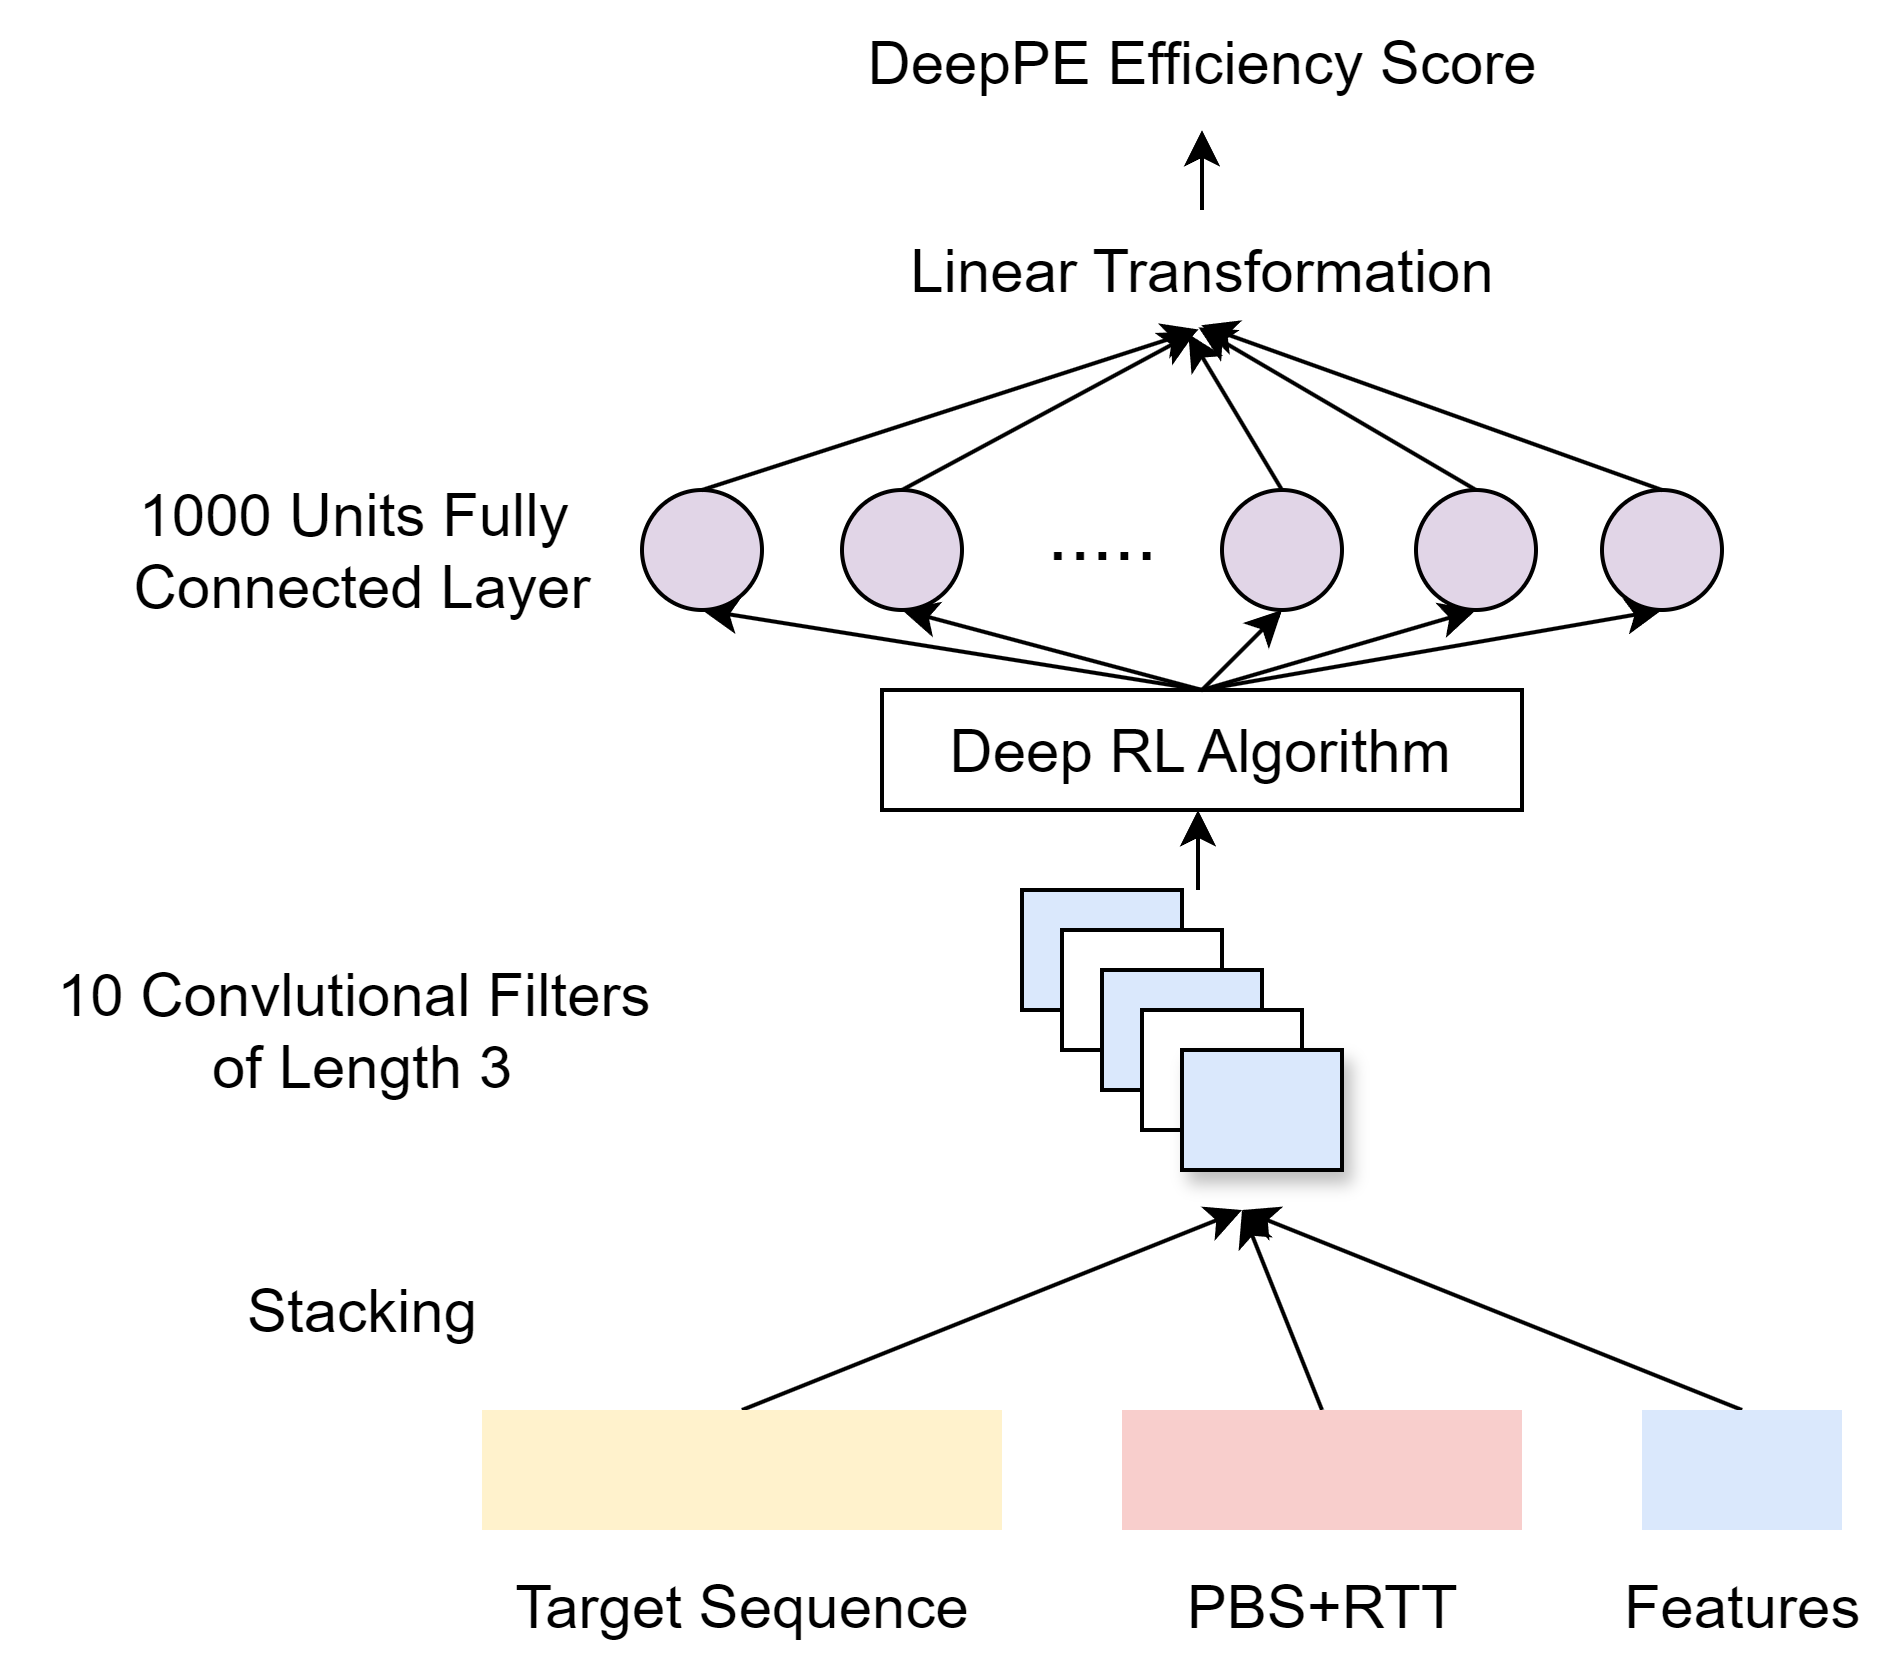
\includegraphics[width=0.6\textwidth]{DeepPE.png}
    \caption{DeepPE Model Architecture}
    \label{fig:deeppe}
\end{figure}

This architecture had the highest performance among the methods reviewed by the authors, although not significantly higher than L1 Lasso regression model. The model achieved a Spearman's R of 0.7 to 0.8, and a Pearson's r of 0.6 to 0.7 on the held-out as well as generalization(unseen) datasets.

The authors also developed another multi-layer perceptron(MLP) model to predict the editing efficiency of more general editing types, including single-nucleotide insertions, deletions and substitutions. However, random forest achieved better performances and was thus used in the additional PE\_Type and PE\_Position models. PE\_Type model proposes pegRNA for 24 possible edits, including specific single-nucleotide deletions, insertions, and substitutions at designated locations. PE\_Position model proposes pegRNA optimized to perform substitutions at ten more positions, namely positions 1, 2, 3, 4, 6, 7, 8, 9, 11 and 14.

\section{Easy Prime}

EasyPrime is a XGBoost regression model developed by Liu et al to produce design for RTT, PBS and ngRNA. Instead of arbitrary mutations, Easy-Prime predicts the editing efficiency of the variants logged in the Genome-Wide Association Studies(GWAS) database. The GWAS variants are the single nucleotide polymorphisms(SNPs) that have been associated with particular traits or diseases.

Similar to DeepPE, for each variant, the web tool proposes a number of pegRNA design using the constrains on PBS, RTT and ngRNA length provided by the user. The proposed pegRNAs are then evaluated by the XGBoost models to find the optimal candidate. When producing the efficiency score, EasyPrime takes the extracted features from pegRNA and target sequences as input to the model instead of the sequences themselves. The extracted features include GC content of the PBS, PAM sequence disruption, as well as several target mutation features describing the mutations to insert.

Cas9 activity score produced by DeepSpCas9 is also used as a feature in the model. DeepSpCas9 is a convolutional neural network model that predicts the activity of the SpCas9 protein on a given target sequence and sgRNA pair. The model architecture is very similar to DeepPE, with one convolutional layer followed by three fully connected layers. The unique feature of the model is the use of filters of different sizes in the convolutional layer(3, 5, and 7nt), allowing the model to capture the dependencies between the base pairs at different distances\cite{kimSpCas9ActivityPrediction2019}.

Albeit limited in the type of edits supported, EasyPrime is one of a few methods that provides official support for ngRNA design required by PE3 and PE3b. Note that PE3b is the optimized version of PE3, where the ngRNA is selected to avoid possible DSB by not targeting the nucleotide complementary to the nicked position\cite{liudavidr.SearchandreplaceGenomeEditing2019}.

Constrained by the data available and the simple architecture of the model, the performance of EasyPrime is relatively low compared to the other models reviewed. The model achieved a Spearman's R and Pearson's r of 0.5 to 0.6 on their held-out datasets.

\section{DeepPrime}

\begin{figure}[ht]
    \centering
    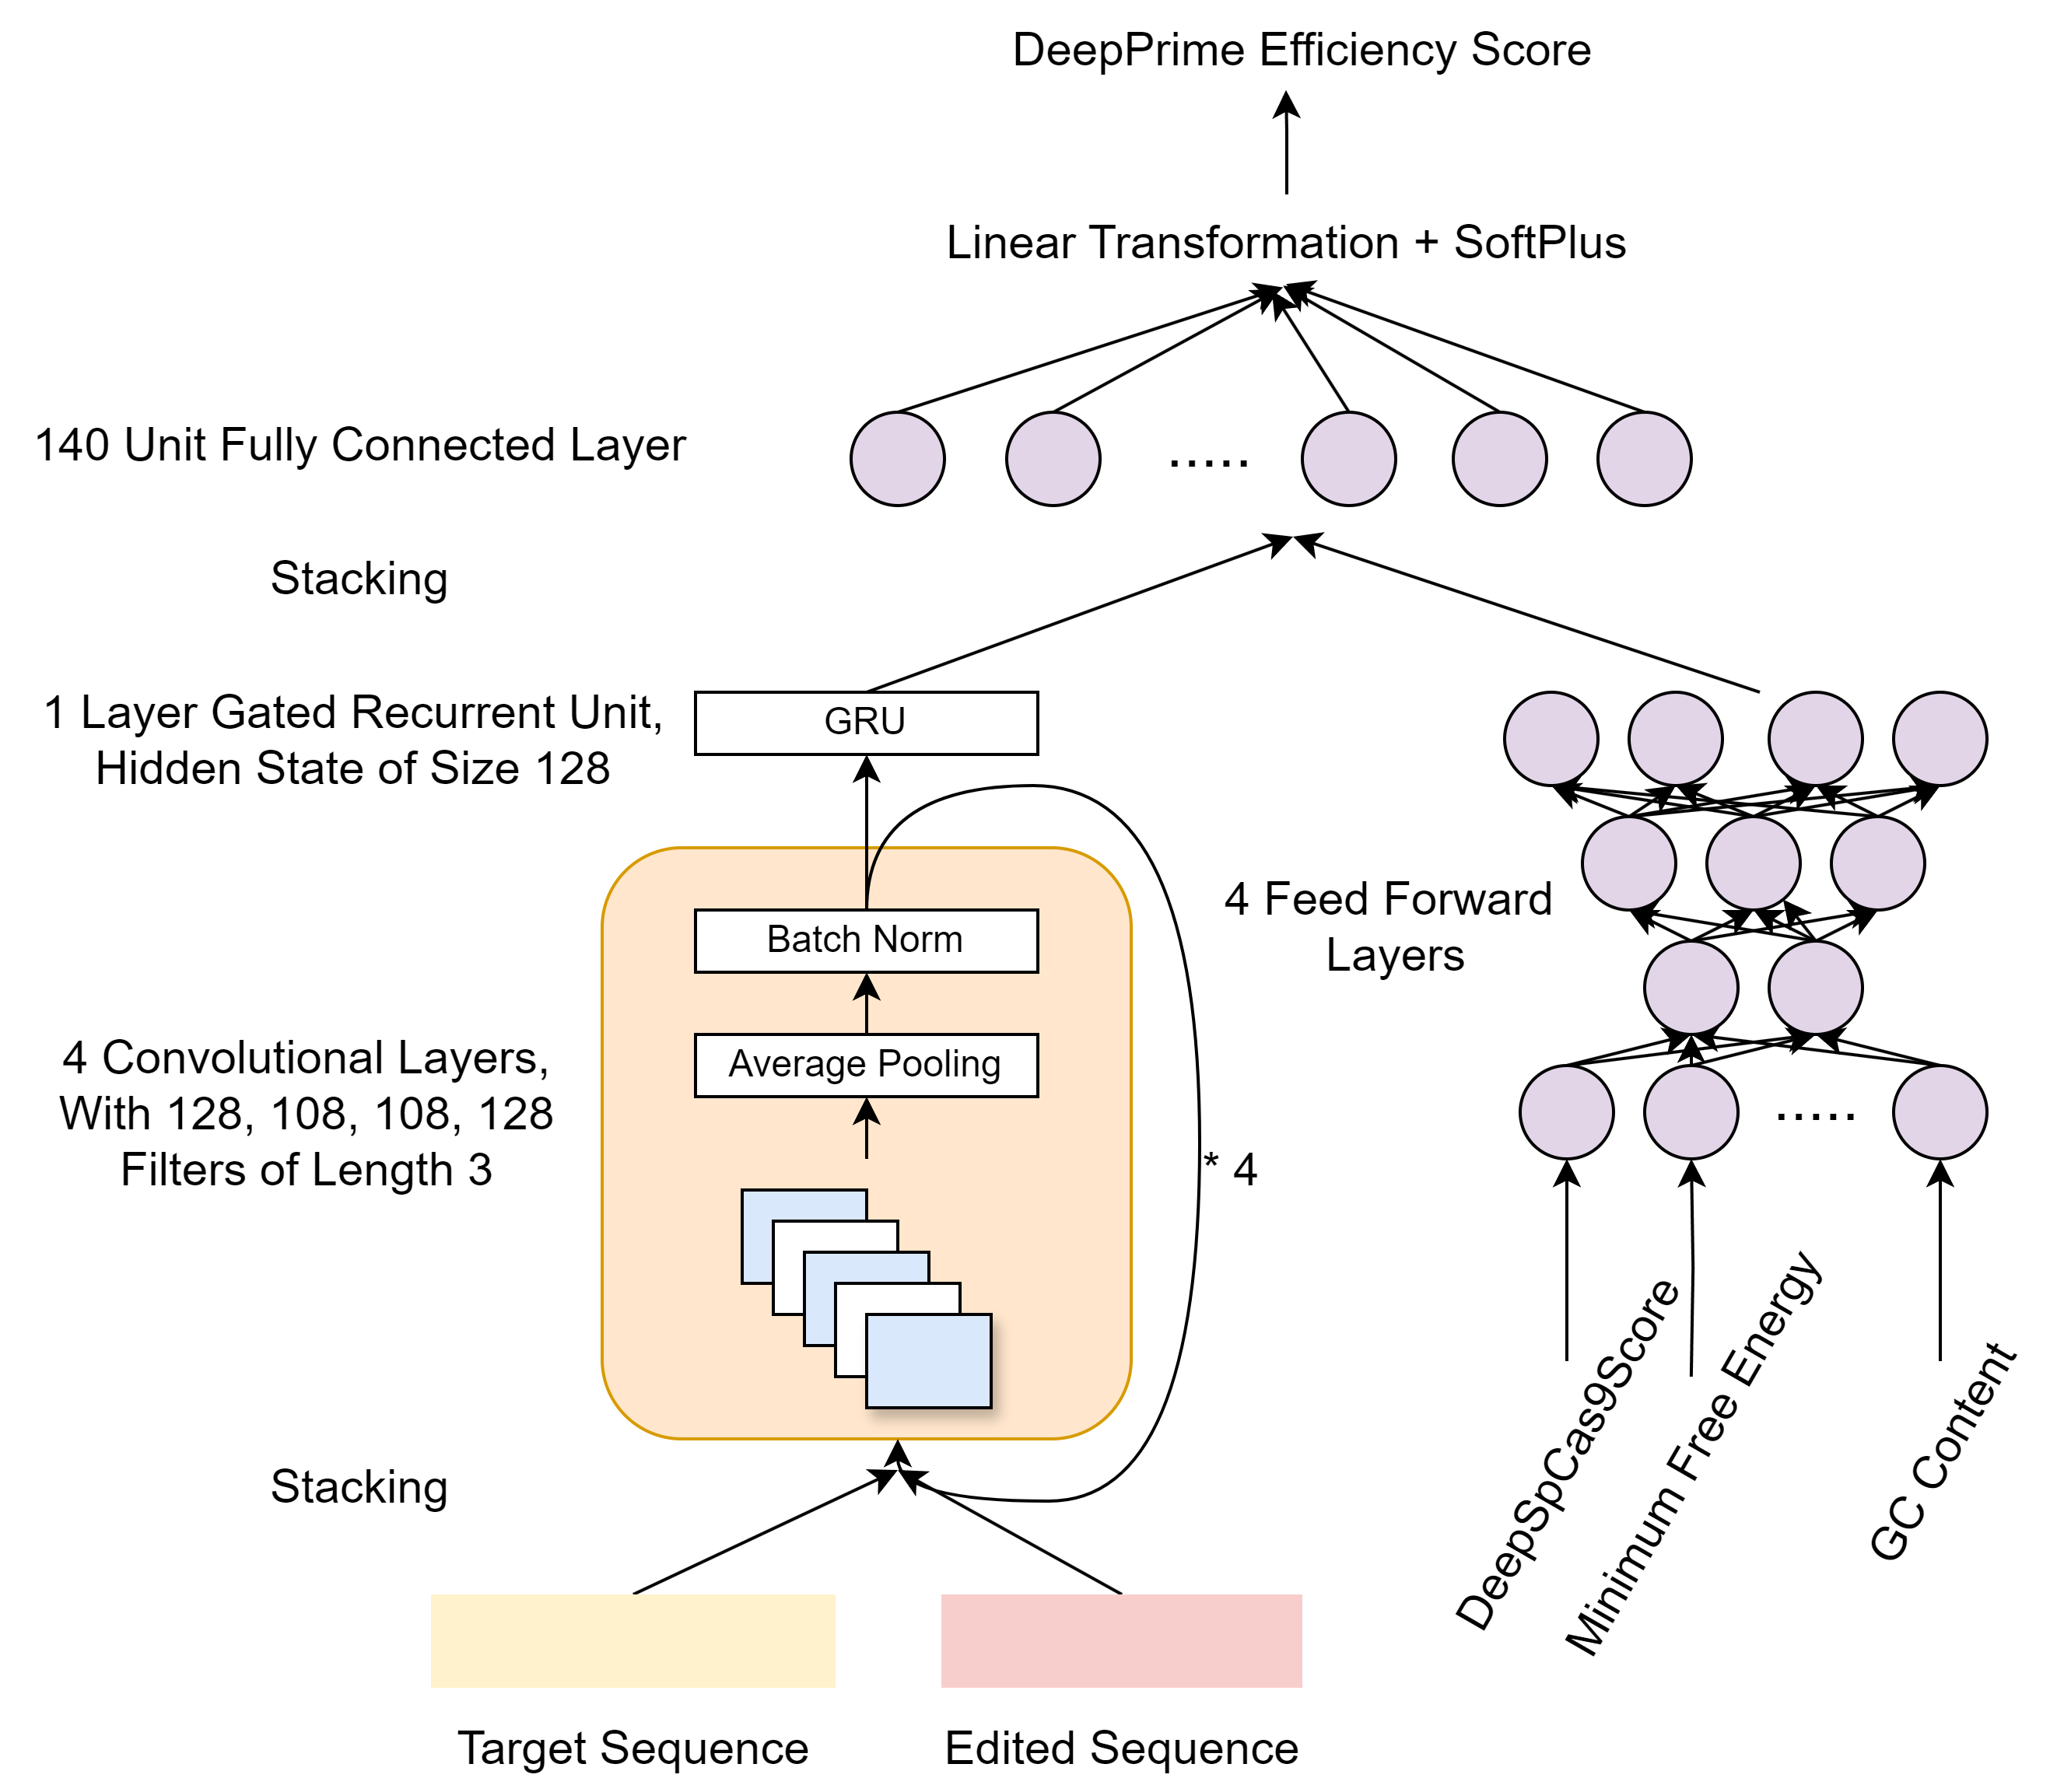
\includegraphics[width=0.8\textwidth]{DeepPrime.png}
    \caption{DeepPrime Model Architecture}
    \label{fig:deepprime}
\end{figure}


Also developed by Kim et al., DeepPrime is the updated version of DeepPE with an upgraded model architecture. 

Illustrated in \autoref{fig:deepprime}, instead of PBS + RTT with target sequence, it takes the wild type(unedited) as well as the edited sequences as input to the CNN. The convolutional network is significantly larger than DeepPE, containing four convolutional layers with 128, 108, 108, and 128 filters, respectively. Moreover, conventional average pooling is used this time round after each convolutional layer instead of a deep RL algorithm. Batch normalization is also applied to accelerate training.  The output of the convolutional layer is then processed by bidirectional Gated Recurrent Units(GRU). 

Instead of processed together with the embedded sequence, features extracted from the proposed pegRNA and target context sequence are processed using a separate four-layer feed forward neural network. The outputs from the two networks are then stacked and fed into a fully connected layer. The result is linearly transformed and processed by a SoftPlus activation function to produce the final prediction score.


DeepPrime is effectively a multi-task learning model, with a base model trained using the combination of 18 datasets of different PE and cell line combinations. The base model is then fine tuned using each of the 18 datasets to produce a task specific model for each setting, collectively named DeepPrime-FT.  

The amount of training data used makes DeepPrime the most comprehensive method in terms of the number of cell lines and PE versions covered. At the same time, the multi-task design allows DeepPrime-FT to utilize the share features between the different PEs and cell lines, and thus achieve very high performance. 

The model has made significant improvement compared to DeepPE, with a Spearman's R of 0.8 to 0.9, and a Pearson's r of 0.7 to 0.9 on most of the testing datasets, including the generalization datasets unseen during training.

\section{PRIDICT}

\begin{figure}[ht]
    \centering
    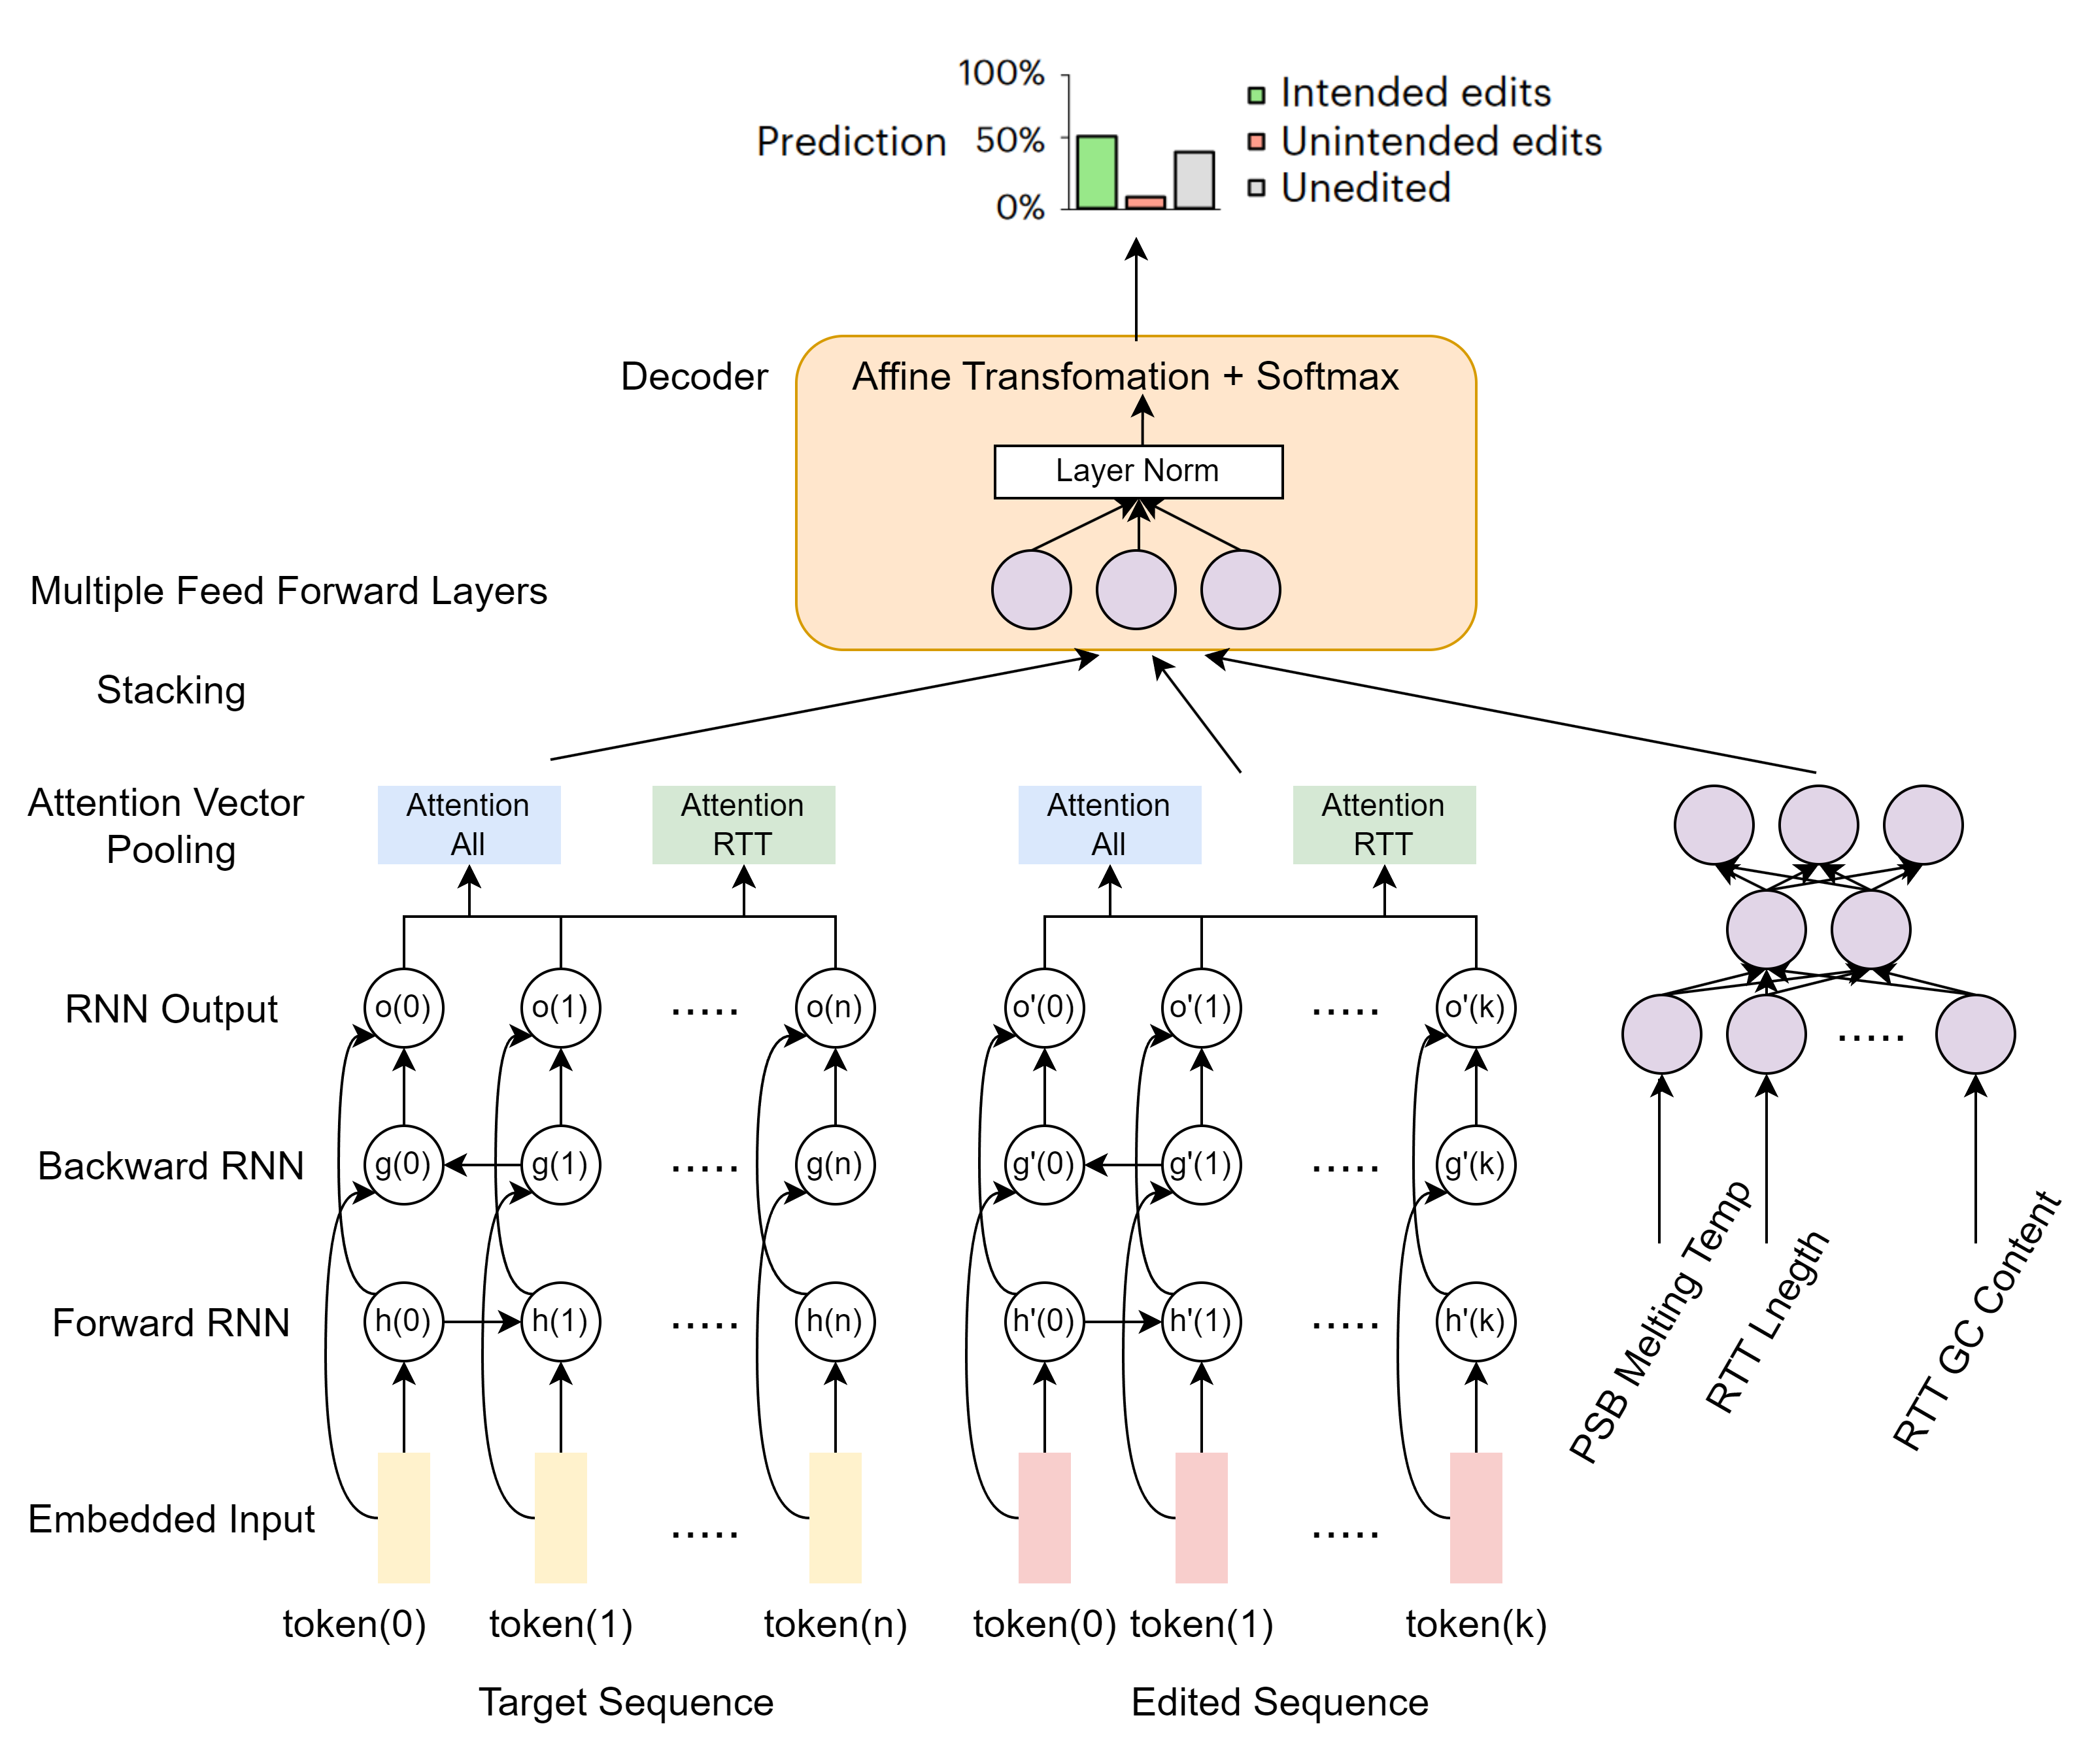
\includegraphics[width=\textwidth]{pridict.png}
    \caption{PRIDICT Model Architecture}
    \label{fig:pridict}
\end{figure}


Developed by Gerald Schwank et al, PRIDICT utilizes a sophisticated attention-based bidirectional RNN model with a similar pegRNA recommendation pipeline to DeepPE and DeepPrime. 

The model overall is a three encoder one decoder architecture. Two of the encoders are attention-based bidirectional RNN models, learning the vector representation of the sequence data. The third encoder is a feed forward neural network taking explicit features derived from the proposed pegRNA, such as the length of the modifications to insert and melting temperature of the PBS, as inputs, similar to DeepPrime.

The target and mutation sequences are one-hot encoded, alongside three additional binary encoding indicating whether the nucleotide belongs to the protospacer, RTT or PBS. The four embeddings are stacked together into a vector of length 9 for each token in the target sequence and 7 for the mutated sequence(the protospacer embedding is omitted for mutated sequence) and fed into the model.

The bidirectional RNN model is used to capture the dependencies between the base pairs within the whole sequence, instead of only past information captured by unidirectional RNN models. Two separate attention query vectors then pools(compresses) sequence of token-level representations into one fixed length vector using the calculated attention weights. One query vector pools all tokens of the sequences, providing context. The other pools only RTT tokens, focusing on the part where the edits are made. 

The decoder is another feed forward neural network with residual connections and layer normalization, taking the pooled vectors from the encoders and calculating the probability distribution of possible outcomes of the edits when using the proposed guide. 

The model architecture is illustrated in \autoref{fig:pridict}.

Significantly higher performance was achieved by PRIDICT when compared to DeepPE (including PE\_Type and PE\_Position) and EasyPrime, with 2-3 fold increase in Spearman's R and Pearson's r on the generalization datasets curated by Gerald et al. PRIDICT also achieved comparable or better results on the datasets DeepPE and EasyPrime were originally trained on. In terms of current generation of models, it was on par with DeepPrime on the HEK293T datasets when predicting intended edits, with a Spearman's R of 0.81. At the same time, PRIDICT outperformed the MinsePIE model as mentioned in section \ref{sec:minsepie}.

\chapter{Full List of Features Invested}
\label{appendix:features}

For individual feature such as tm-pbs, $\checkmark$ indicates that the feature was used in the final model and $\times$ indicates that the feature was not used in the final model. At the same time, for a group of features, if at least one feature was used in the final model, a $\circ$ is placed in the last column. 

% table of features and their explanations
\begin{table}[ht]
    \centering
    \begin{tabular}{|p{0.3\textwidth}|p{0.5\textwidth}|p{0.1\textwidth}|}
        \hline
        \textbf{Feature} & \textbf{Explanation} & \textbf{Top 24} \\ 
        \hline
        tm-pbs& Melting temperature fo pbs RNA sequences & $\checkmark$ \\
        \hline
        tm-rt& Melting temperature of RT primer RNA sequences & $\times$ \\
        \hline
        tm-spacer& Melting temperature of spacer RNA sequences & $\checkmark$ \\
        \hline
        max-cas & Maximum number of consecutive A bases in the cDNA of extension as well as protospacer sequence & $\times$ \\
        \hline
        max-cts & Maximum number of consecutive T bases in the cDNA of extension as well as protospacer sequence & $\checkmark$ \\
        \hline
        max-cgs & Maximum number of consecutive G bases in the cDNA of extension as well as protospacer sequence & $\times$ \\
        \hline
        max-ccs & Maximum number of consecutive C bases in the cDNA of extension as well as protospacer sequence & $\times$ \\
        \hline
    \end{tabular}
\end{table}

% table of features and their explanations
\begin{table}[ht]
    \centering
    \begin{tabular}{|p{0.3\textwidth}|p{0.5\textwidth}|p{0.1\textwidth}|}
        \hline
        \textbf{Feature} & \textbf{Explanation} & \textbf{Top 24} \\ 
        \hline
        mfe-pbs & Minimum free energy of pbs RNA sequences & $\checkmark$ \\
        \hline
        mfe-rt & Minimum free energy of RT primer RNA sequences & $\times$ \\
        \hline
        mfe-spacer & Minimum free energy of spacer RNA sequences & $\checkmark$ \\
        \hline
    \end{tabular}
\end{table}

\chapter{Fine Tuning the Transformer Model}
\label{appendix:transformer-hyperparameter-tuning}

Full result of the hyperparameter tuning for the transformer model.

\begin{longtable}{|>{\raggedright\arraybackslash}p{2cm}|>{\raggedright\arraybackslash}p{2cm}|>{\raggedright\arraybackslash}p{2cm}|>{\raggedright\arraybackslash}p{3.5cm}|>{\raggedright\arraybackslash}p{2cm}|>{\raggedright\arraybackslash}p{2cm}|}
    \hline
    \textbf{MLP Embed Dim} & \textbf{Num Encoder Units} & \textbf{Dropout} & \textbf{Performance} & \textbf{Mean} & \textbf{Max} \\
    \hline
    \endfirsthead
    
    \hline
    \textbf{MLP Embed Dim} & \textbf{Num Encoder Units} & \textbf{P Dropout} & \textbf{Performance} & \textbf{Mean Performance} & \textbf{Max Performance} \\
    \hline
    \endhead
    
    \hline
    \endfoot
    
    100 & 1 & 0.1 & [0.8039, 0.8214, 0.8204, 0.7896, 0.7923] & 0.8055 & 0.8214 \\
    \hline
    100 & 1 & 0.3 & [0.8062, 0.8024, 0.8111, 0.8009, 0.8258] & 0.8093 & 0.8258 \\
    \hline
    100 & 1 & 0.5 & [0.7753, 0.7982, 0.7899, 0.8025, 0.7869] & 0.7906 & 0.8025 \\
    \hline
    100 & 2 & 0.1 & [0.8035, 0.8024, 0.7926, 0.8187, 0.7899] & 0.8014 & 0.8187 \\
    \hline
    100 & 2 & 0.3 & [0.8137, 0.8168, 0.8014, 0.7962, 0.7909] & 0.8038 & 0.8168 \\
    \hline
    100 & 2 & 0.5 & [0.7986, 0.8008, 0.7874, 0.7776, 0.7771] & 0.7883 & 0.8008 \\
    \hline
    100 & 3 & 0.1 & [0.7995, 0.8001, 0.8015, 0.8003, 0.8128] & 0.8028 & 0.8128 \\
    \hline
    100 & 3 & 0.3 & [0.7879, 0.8043, 0.7797, 0.7929, 0.7939] & 0.7917 & 0.8043 \\
    \hline
    100 & 3 & 0.5 & [0.7735, 0.7864, 0.7758, 0.7888, 0.7847] & 0.7818 & 0.7888 \\
    \hline
    150 & 1 & 0.1 & [0.8047, 0.8202, 0.8059, 0.8001, 0.7957] & 0.8053 & 0.8202 \\
    \hline
    150 & 1 & 0.3 & [0.8195, 0.8171, 0.8085, 0.7845, 0.7858] & 0.8031 & 0.8195 \\
    \hline
    150 & 1 & 0.5 & [0.7554, 0.7521, 0.7853, 0.7884, 0.7979] & 0.7758 & 0.7979 \\
    \hline
    150 & 2 & 0.1 & [0.7995, 0.8025, 0.7994, 0.7979, 0.7990] & 0.7996 & 0.8025 \\
    \hline
    150 & 2 & 0.3 & [0.7998, 0.7934, 0.7941, 0.8122, 0.8094] & 0.8018 & 0.8122 \\
    \hline
    150 & 2 & 0.5 & [0.7938, 0.7935, 0.7799, 0.7985, 0.7643] & 0.7860 & 0.7985 \\
    \hline
    150 & 3 & 0.1 & [0.8033, 0.7837, 0.8062, 0.8033, 0.8046] & 0.8002 & 0.8062 \\
    \hline
    150 & 3 & 0.3 & [0.7946, 0.7983, 0.7940, 0.8186, 0.7984] & 0.8008 & 0.8186 \\
    \hline
    150 & 3 & 0.5 & [0.7756, 0.7873, 0.7961, 0.7878, 0.7923] & 0.7878 & 0.7961 \\
    \hline
    200 & 1 & 0.1 & [0.8007, 0.8062, 0.8216, 0.8095, 0.8182] & 0.8112 & 0.8216 \\
    \hline
    200 & 1 & 0.3 & [0.7820, 0.8164, 0.7751, 0.8053, 0.8172] & 0.7992 & 0.8172 \\
    \hline
    200 & 1 & 0.5 & [0.7951, 0.7843, 0.7835, 0.7956, 0.8046] & 0.7926 & 0.8046 \\
    \hline
    200 & 2 & 0.1 & [0.8058, 0.7912, 0.7984, 0.8011, 0.7862] & 0.7965 & 0.8058 \\
    \hline
    200 & 2 & 0.3 & [0.7999, 0.7955, 0.7863, 0.8036, 0.7992] & 0.7969 & 0.8036 \\
    \hline
    200 & 2 & 0.5 & [0.7867, 0.7715, 0.7559, 0.7856, 0.7680] & 0.7735 & 0.7867 \\
    \hline
    200 & 3 & 0.1 & [0.8040, 0.8018, 0.8117, 0.8252, 0.8054] & 0.8096 & 0.8252 \\
    \hline
    200 & 3 & 0.3 & [0.8034, 0.7934, 0.7644, 0.8073, 0.7846] & 0.7906 & 0.8073 \\
    \hline
    200 & 3 & 0.5 & [0.7701, 0.7940, 0.7706, 0.7858, 0.7865] & 0.7814 & 0.7940 \\
    \hline
    \caption{Transformer model's performance using different hyperparameters controlling the parameter size. The hyperparameters are the MLP Embedding Dimension (number of hidden units in the positional feedforward network), Number of Encoder Units (number of transformer layers to stack), and the Dropout Rate. The raw performance as well as the mean and maximum performance are shown.} 
    \end{longtable}
    


\chapter{Additional Figures}
\label{appendix:additional-figures}

\section{Additional Figures for Error Analysis}
\label{appendix:error-analysis-figures}



\begin{figure}[ht]
    \centering
    \subfigure[][Error Distribution]{
        \centering
        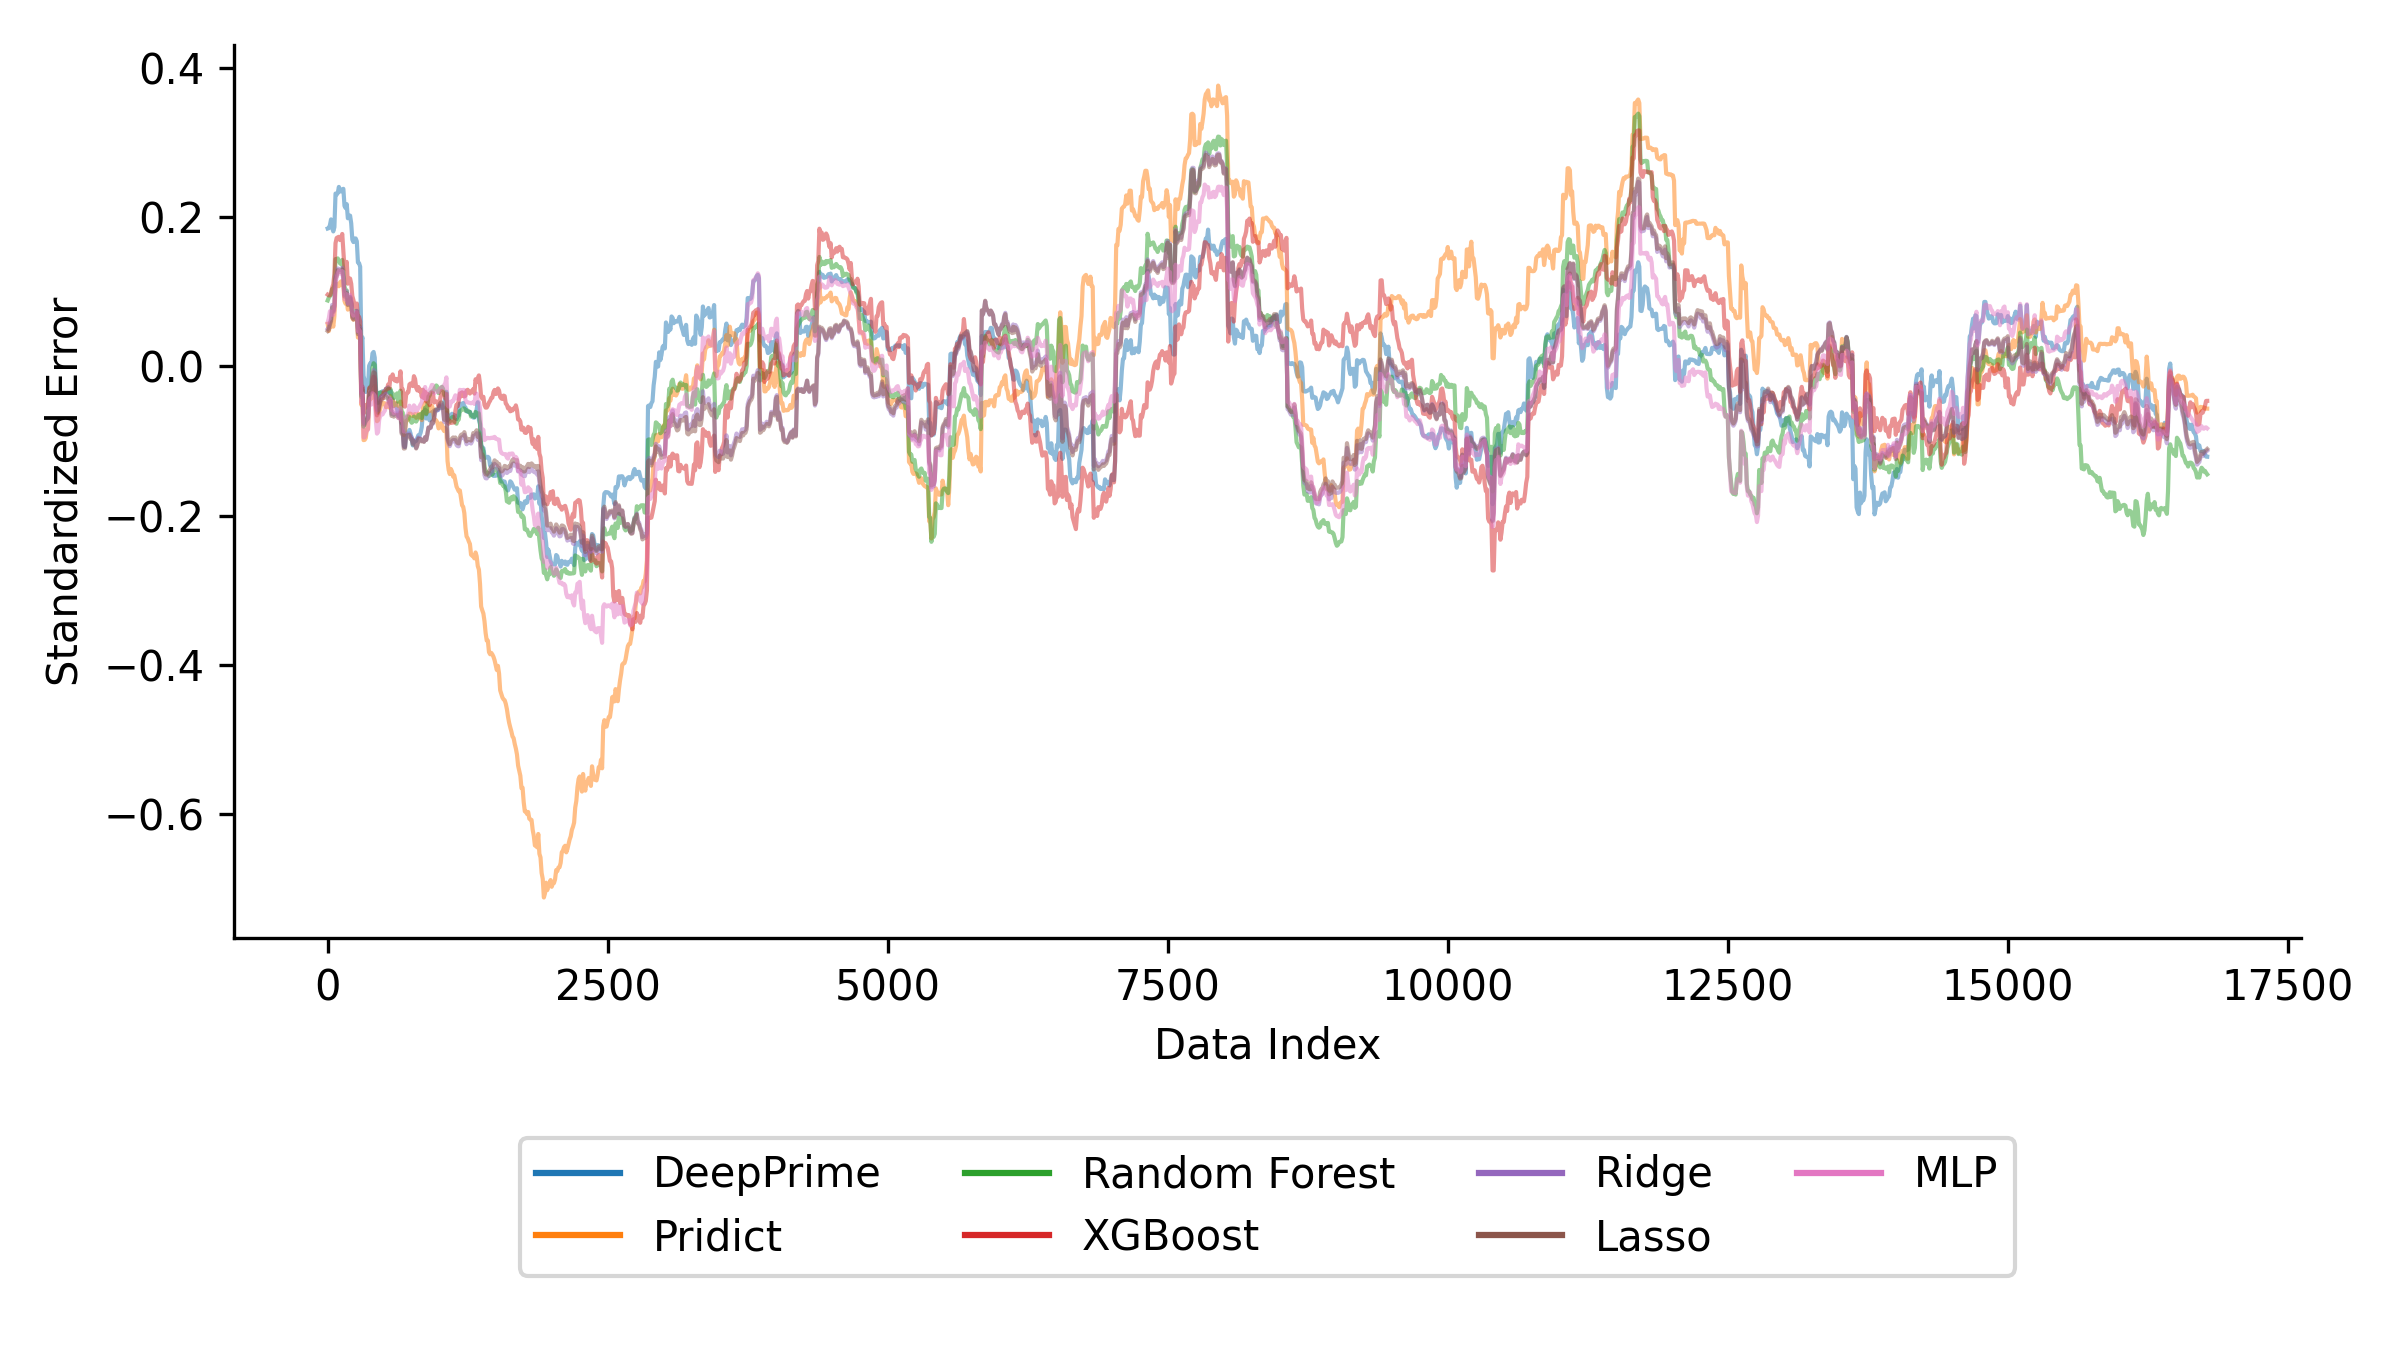
\includegraphics[width=\textwidth]{error_comparison_pd-adv-pe2.png}
        % \caption{Error Distribution of the Individual Models}
        \label{fig:error-distribution-adv-pe2}
    }
    \subfigure[][Pearson Correlation]{
        \centering
        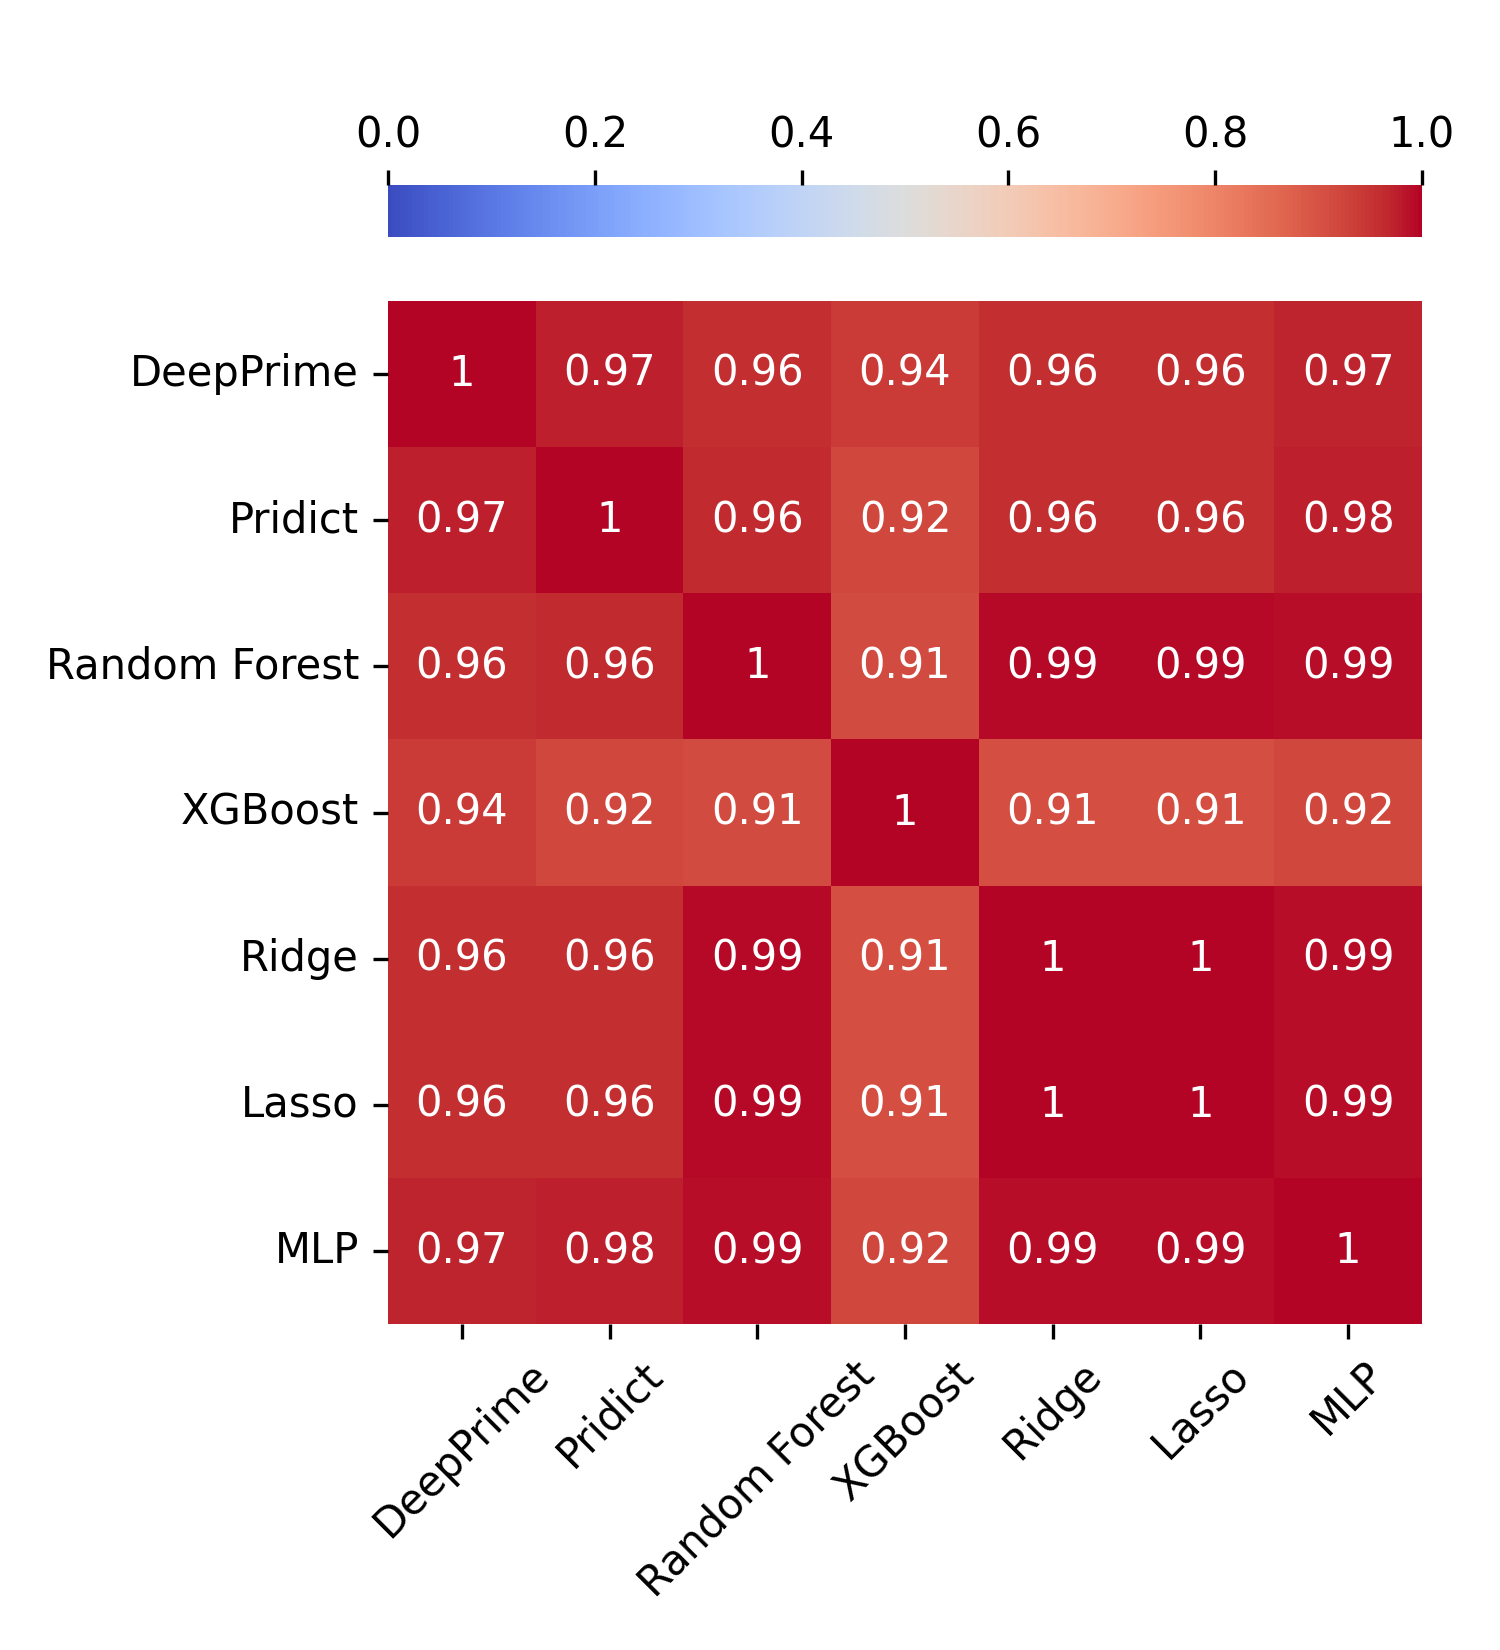
\includegraphics[width=0.49\textwidth]{error_correlation_pd-adv-pe2_pearson.png}
        % \caption{Pearson Correlation of the Error of the Individual Models}
        \label{fig:pearson-correlation-adv-pe2}
    }%
    \subfigure[][Spearman Correlation]{
        \centering
        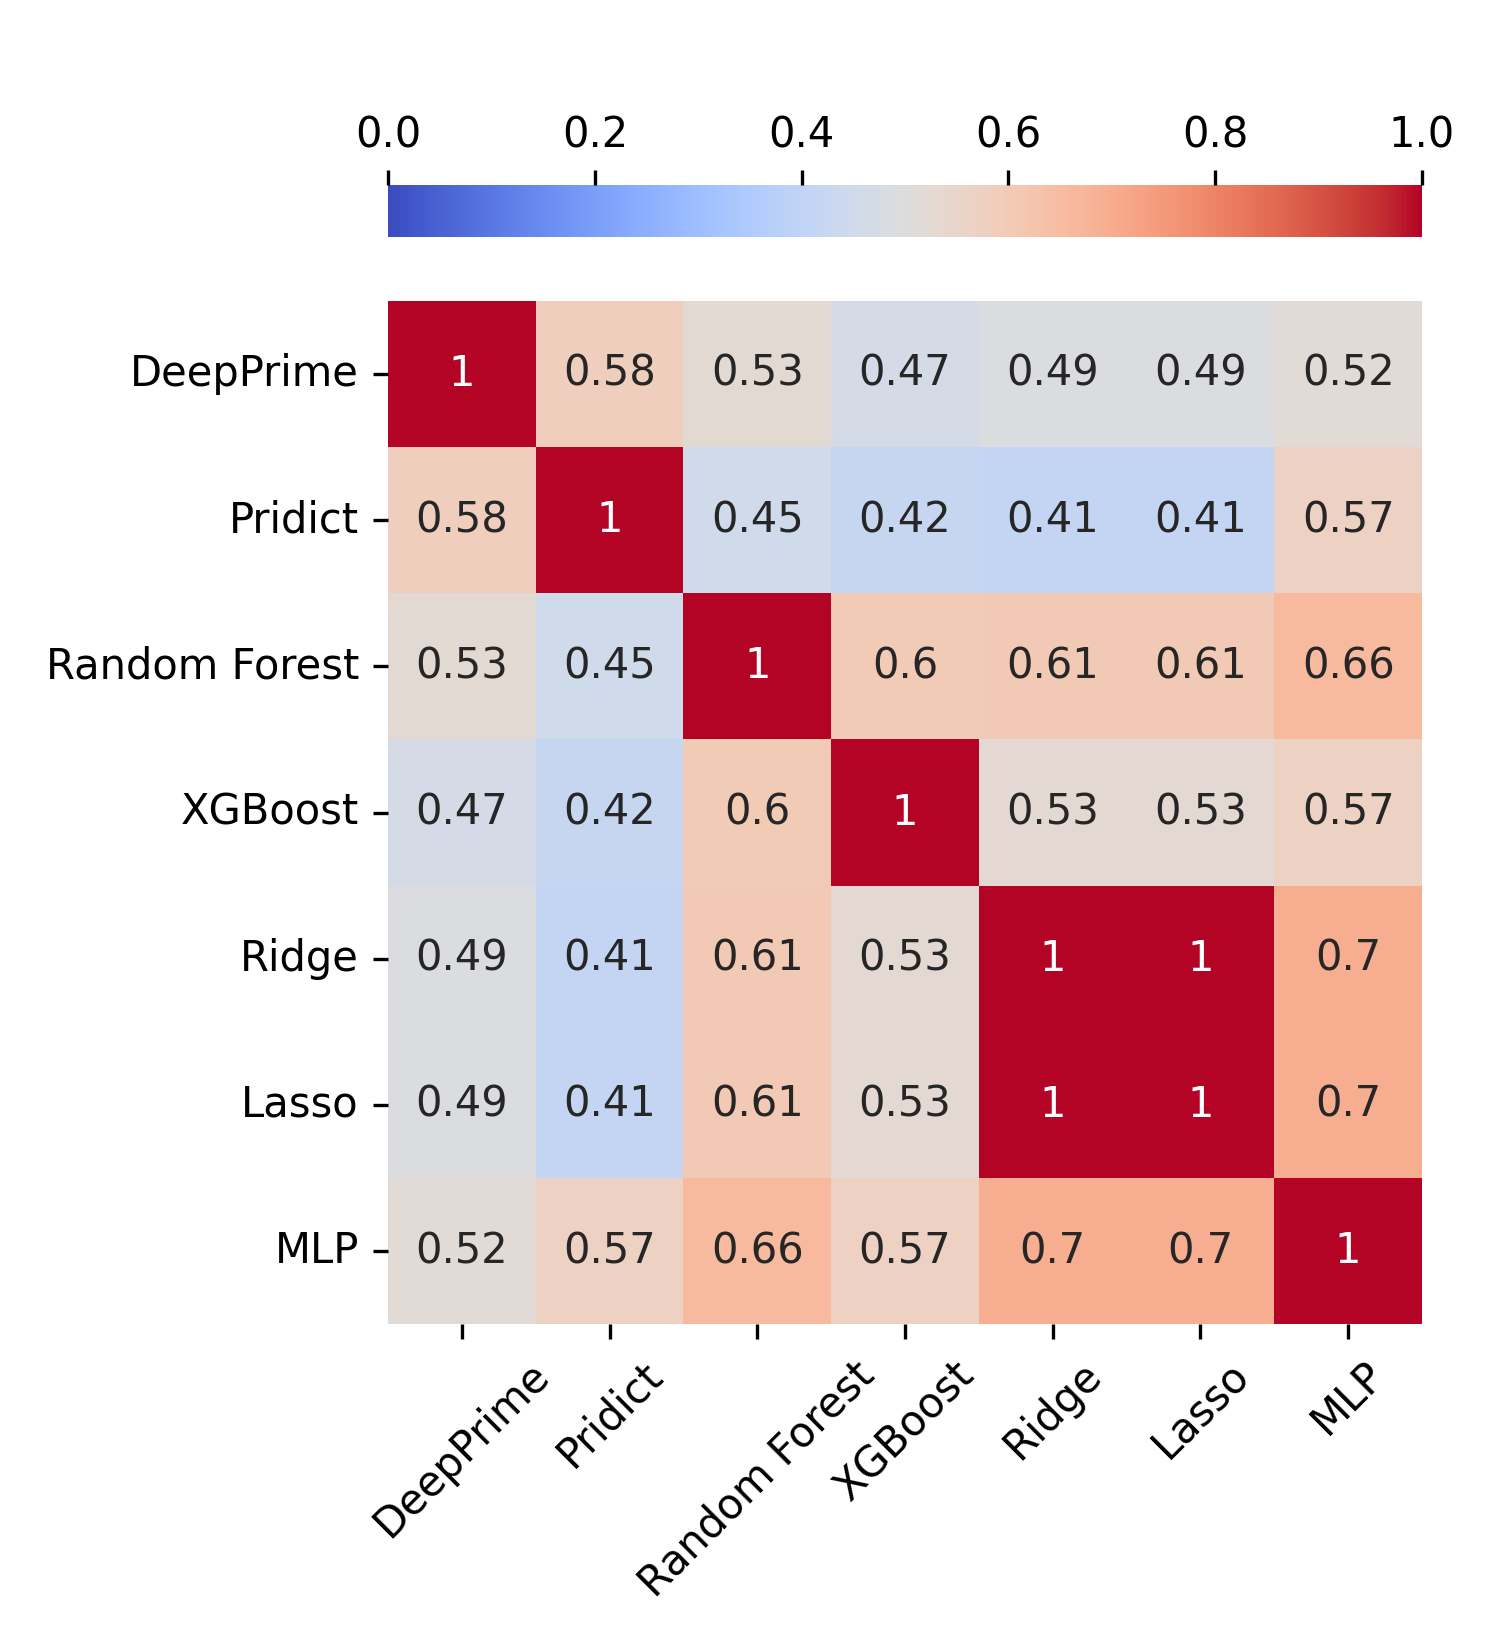
\includegraphics[width=0.49\textwidth]{error_correlation_pd-adv-pe2_spearman.png}
        % \caption{Spearman Correlation of the Error of the Individual Models}
        \label{fig:spearman-correlation-adv-pe2}
    }
    \caption[Error Analysis of the Individual Models on PRIDICT Adv PE2 dataset]{Error Analysis of the Individual Models on the PRIDICT Adv PE2 dataset. \textbf{(a)} The distribution of the error of the individual models at each example, smoothened using a moving window of size 100, and downsampled with a ratio of 10:1 for better visibility; \textbf{(b)} The Pearson correlation of the error of the individual models. \textbf{(c)} The Spearman correlation of the error of the individual models.}
    \label{fig:error-analysis-adv-pe2}
\end{figure}

The same error analysis conducted on \autoref{fig:error-analysis} was also conducted on the PRIDICT datasets. The result is very similar, but with major difference in terms of the correlation between PRIDICT and DeepPrime. The correlation between the two deep learning is much weaker, with the Spearman correlation around 0.7. The more dataset specific differences are pointed out in the caption of \autoref{fig:error-analysis-adv-pe2}, \autoref{fig:error-analysis-hek293t-pe2}, \autoref{fig:error-analysis-k562-pe2}, and \autoref{fig:error-analysis-k562mlh1dn-pe2}.

Due to the smaller data size, the downsampling and smoothing were done with a lower ratio of 10:1 and a smaller moving window of size 100, respectively. 

\begin{figure}
    \centering
    \subfigure[][Error Distribution]{
        \centering
        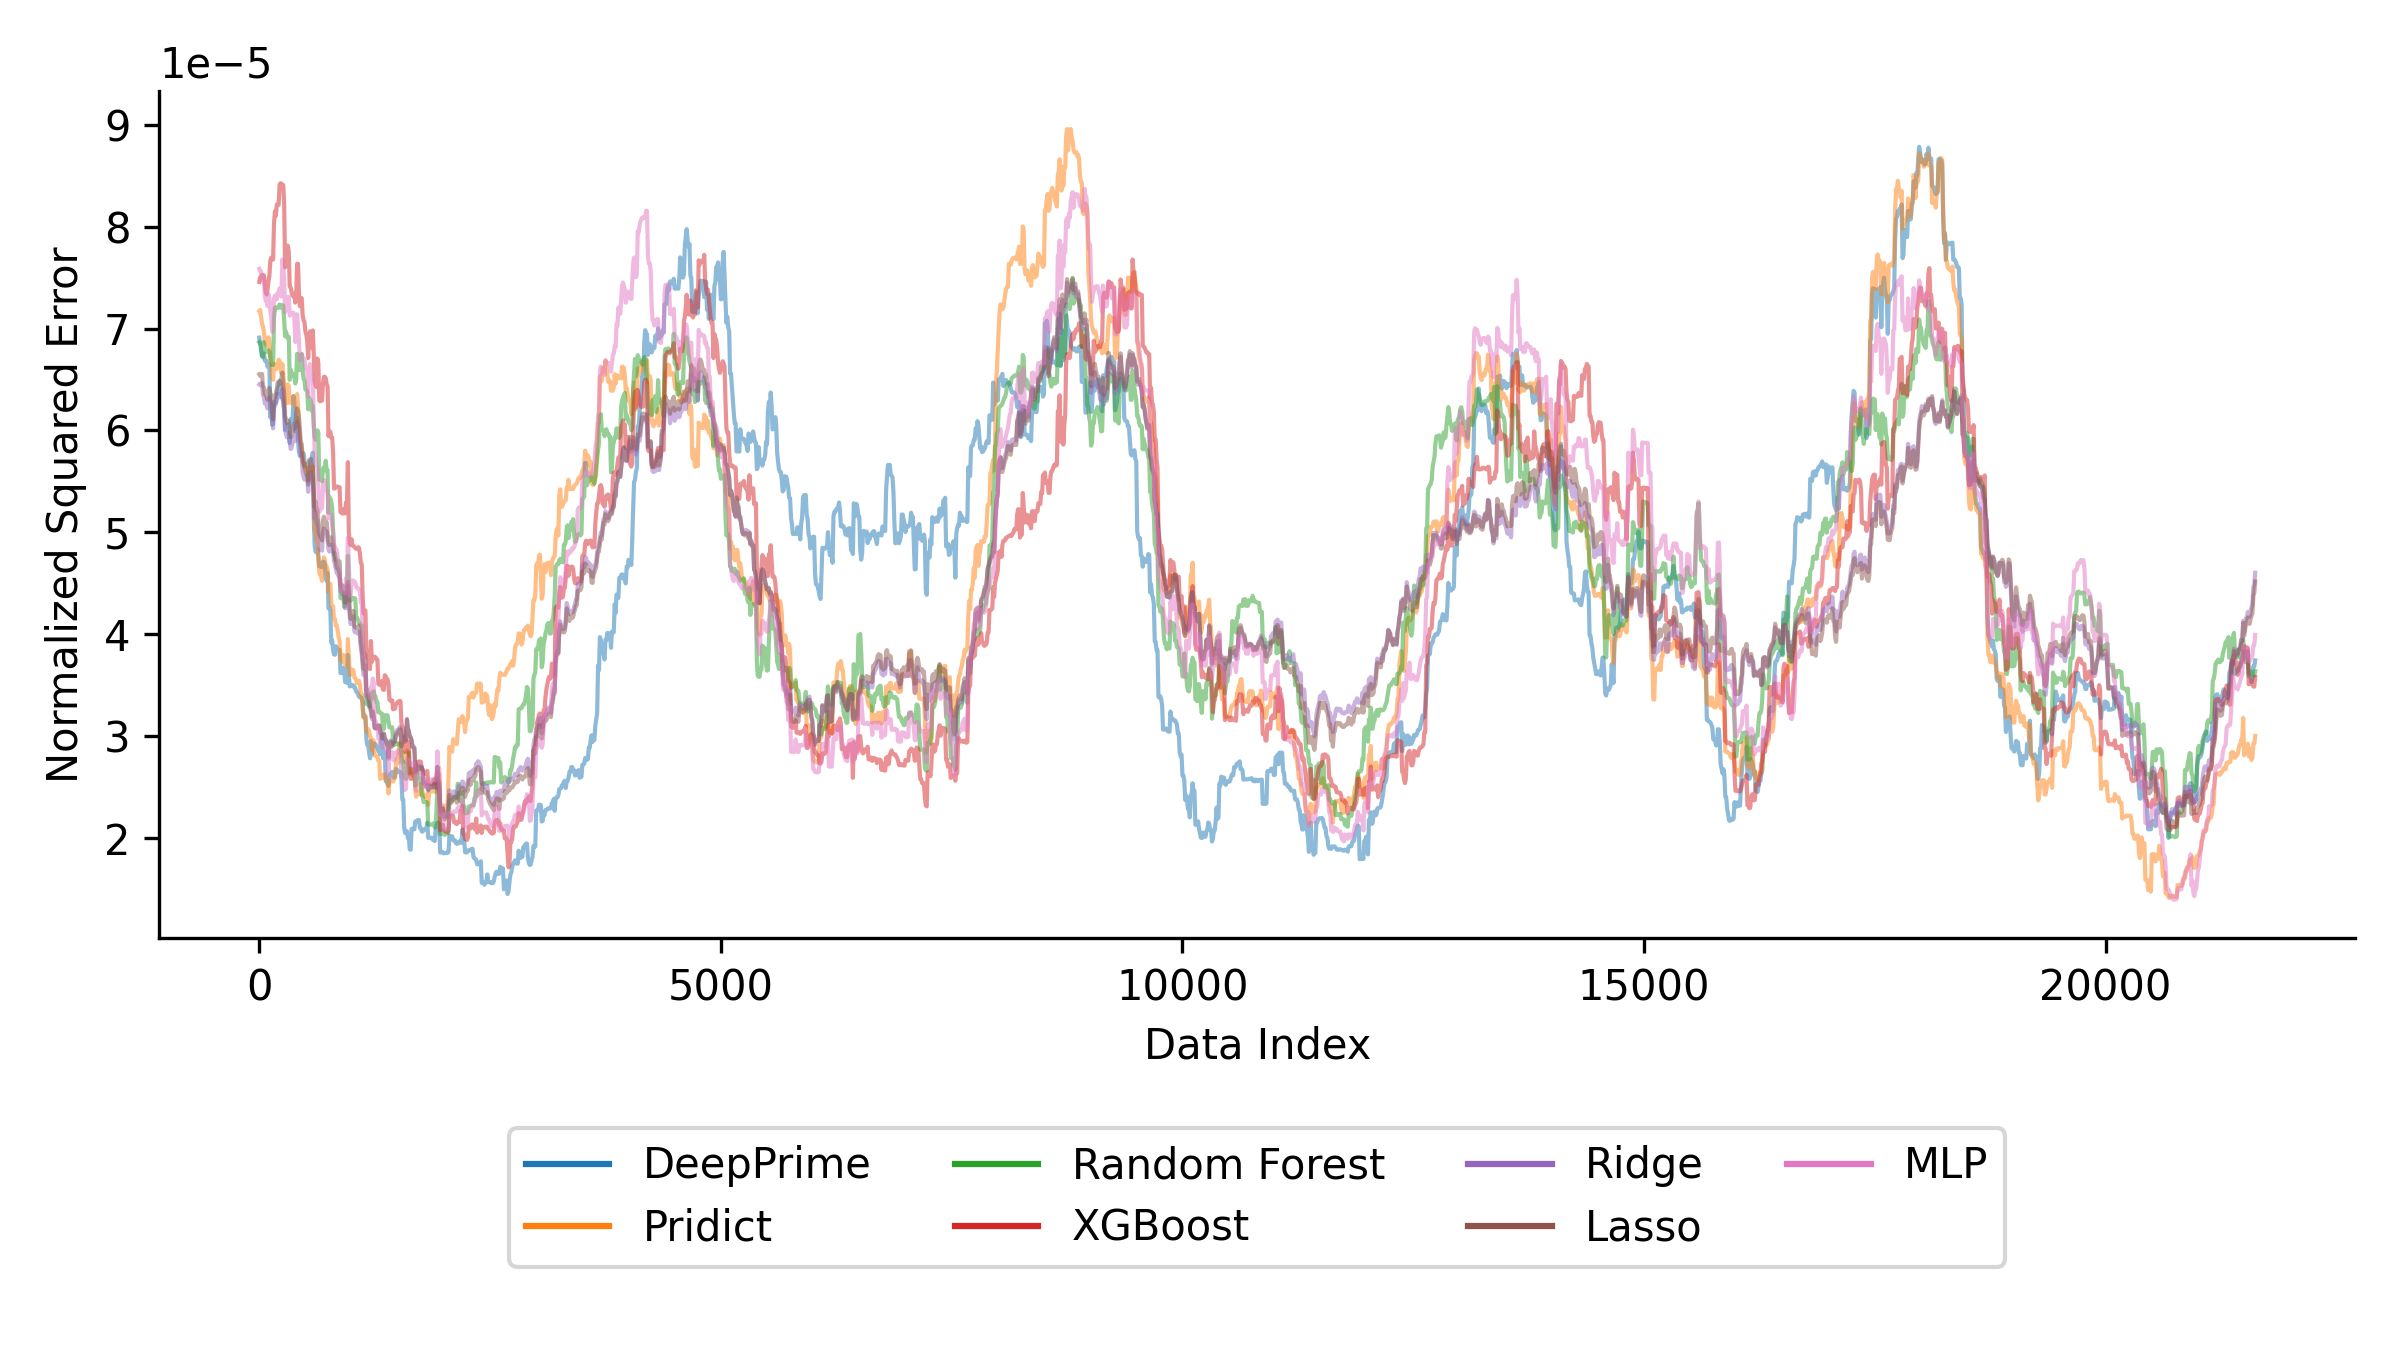
\includegraphics[width=\textwidth]{error_comparison_pd-hek293t-pe2.png}
        % \caption{Error Distribution of the Individual Models}
        \label{fig:error-distribution-hek293t-pe2}
    }
    \subfigure[][Pearson Correlation]{
        \centering
        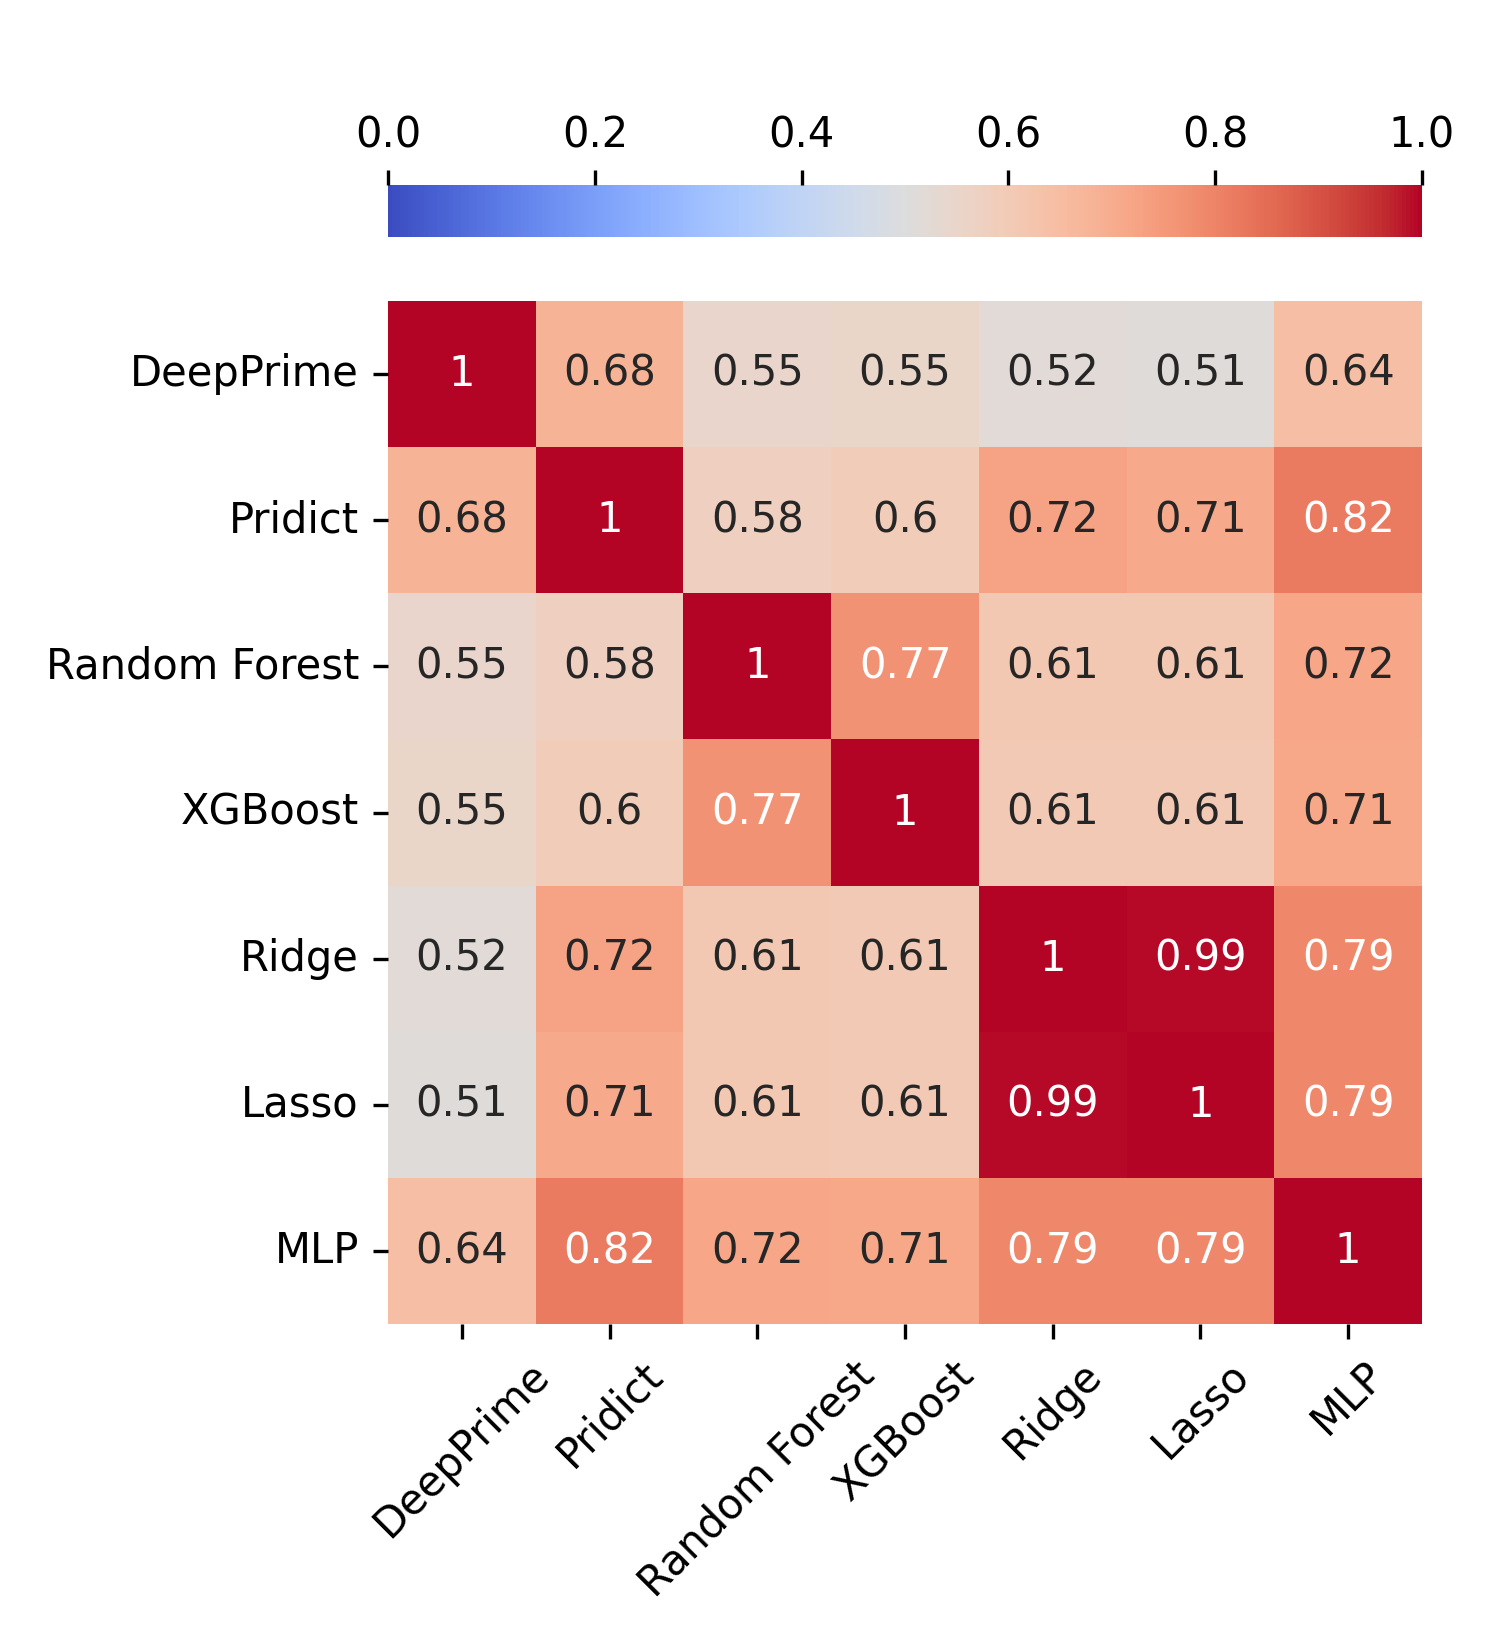
\includegraphics[width=0.49\textwidth]{error_correlation_pd-hek293t-pe2_pearson.png}
        % \caption{Pearson Correlation of the Error of the Individual Models}
        \label{fig:pearson-correlation-hek293t-pe2}
    }%
    \subfigure[][Spearman Correlation
    ]{
        \centering
        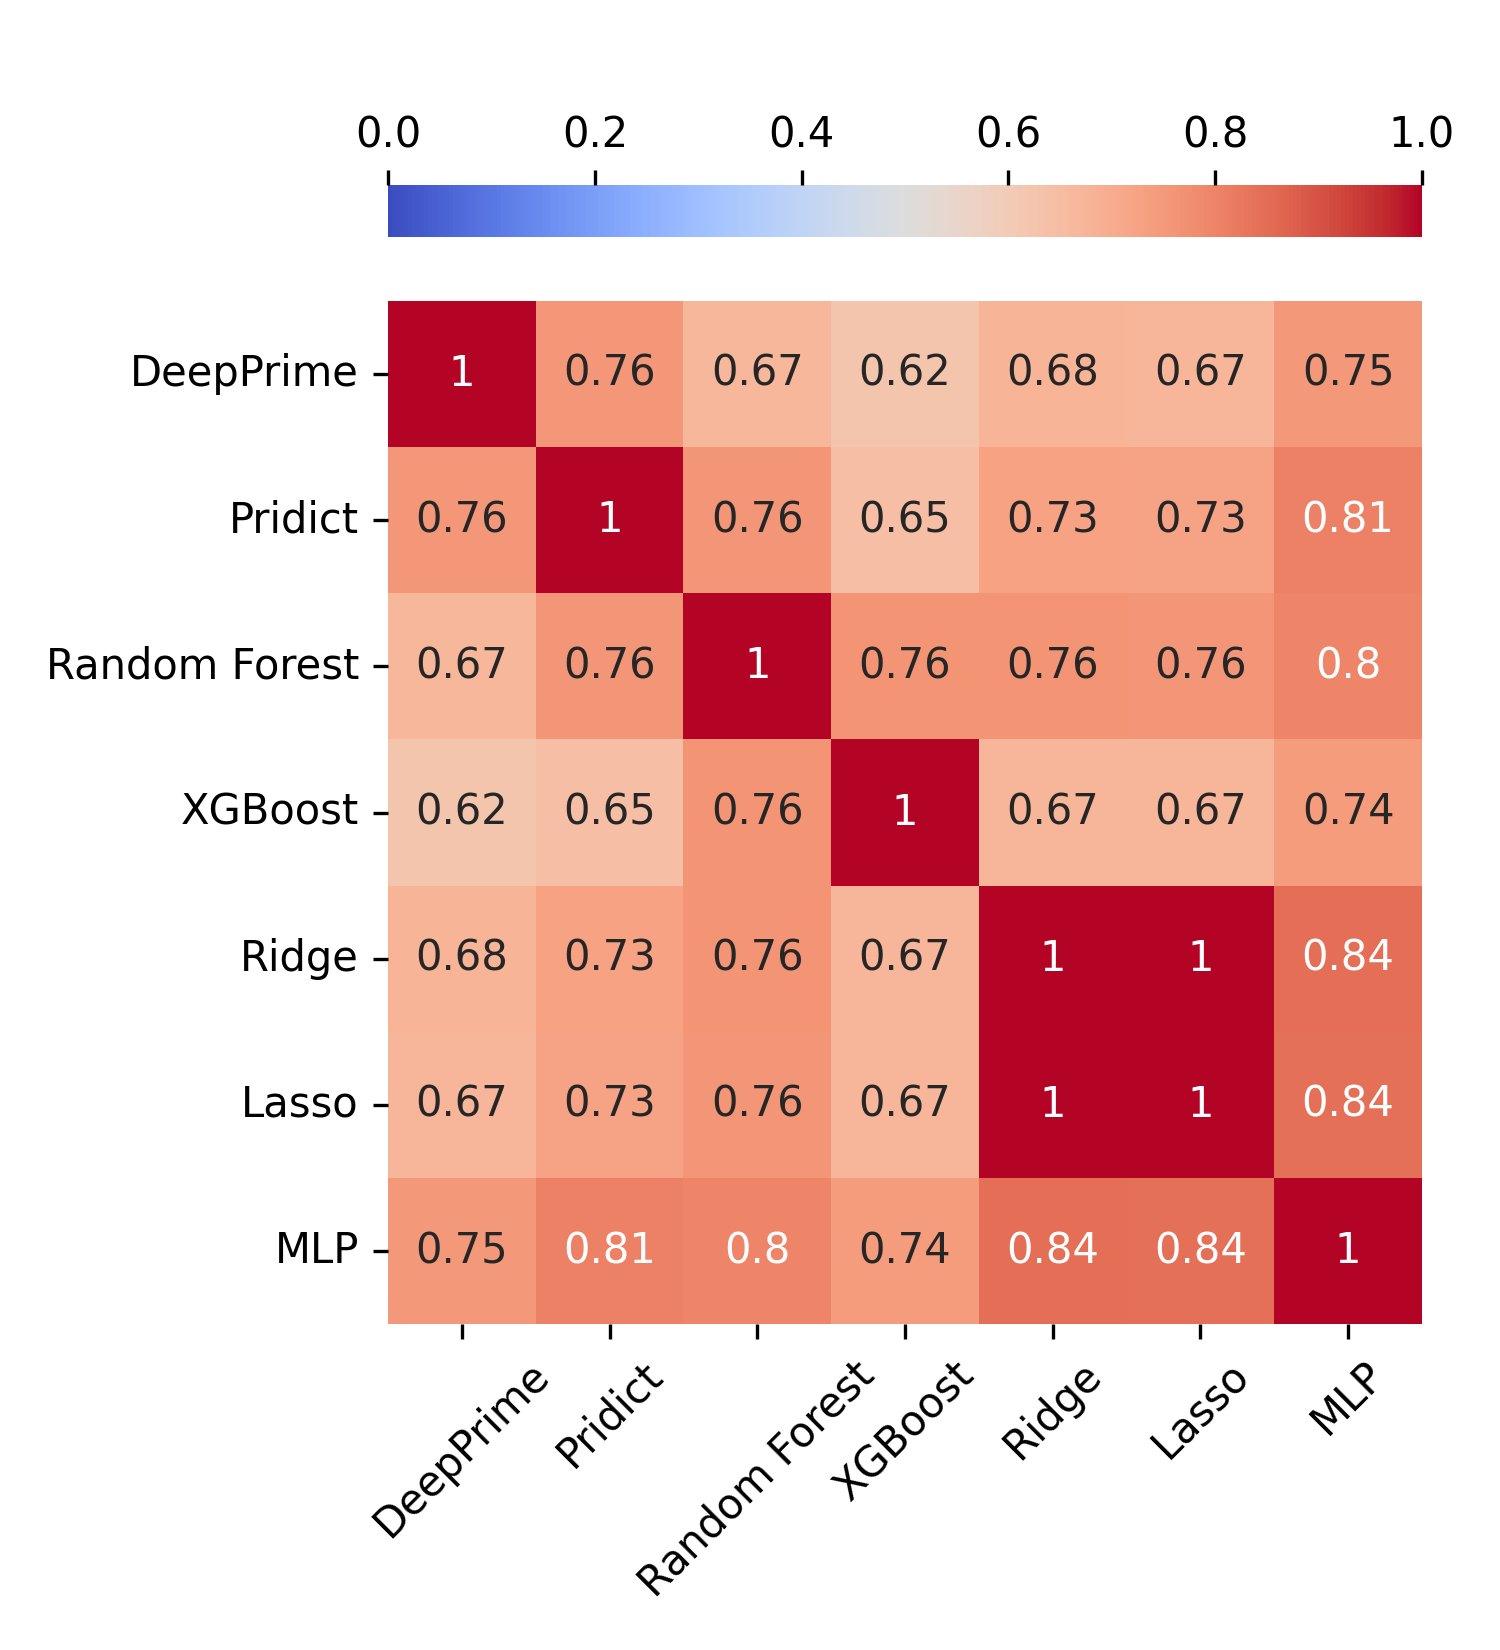
\includegraphics[width=0.49\textwidth]{error_correlation_pd-hek293t-pe2_spearman.png}
        % \caption{Spearman Correlation of the Error of the Individual Models}
        \label{fig:spearman-correlation-hek293t-pe2}
    }
    \caption[Error Analysis of the Individual Models on PRIDICT HEK293T PE2 dataset]{Error Analysis of the Individual Models on the PRIDICT HEK293T PE2 dataset. \textbf{(a)}, \textbf{(b)}, and \textbf{(c)} are the same as \autoref{fig:error-analysis-adv-pe2}. Pearson's r is much weaker, possibly due to a more balanced target value distribution as we have seen in \autoref{fig:imbalanced} The MLP is strongly correlated with all other models, especially PRIDICT.}
    \label{fig:error-analysis-hek293t-pe2}
\end{figure}

\begin{figure}
    \centering
    \subfigure[][Error Distribution]{
        \centering
        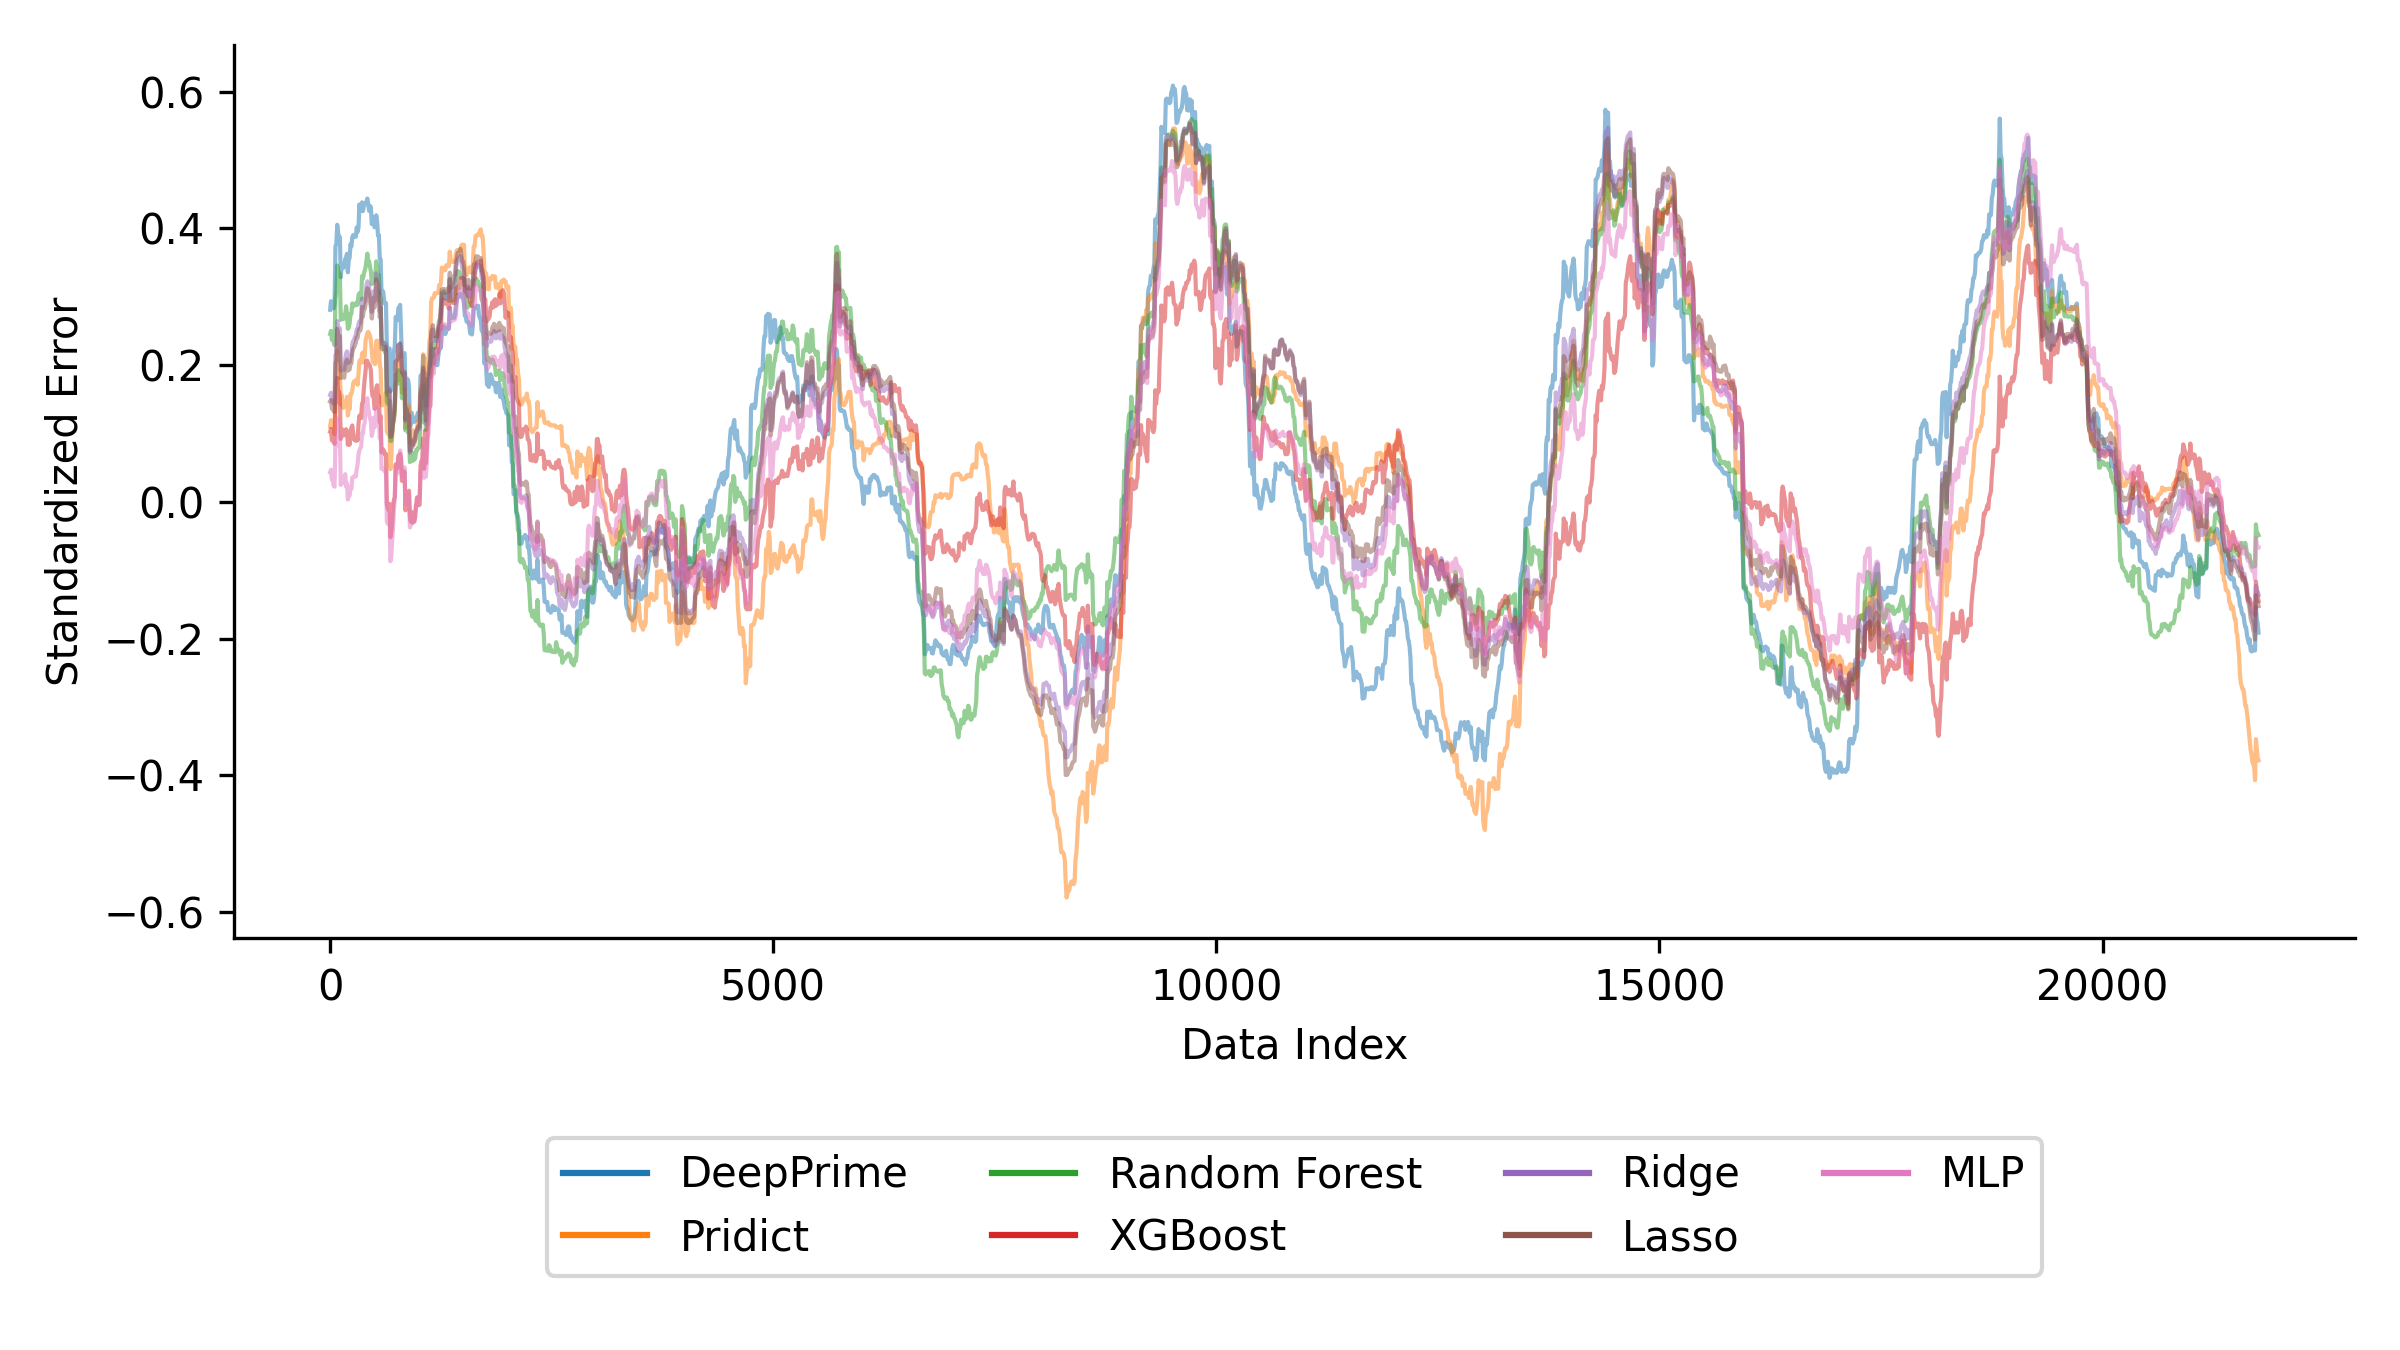
\includegraphics[width=\textwidth]{error_comparison_pd-k562-pe2.png}
        % \caption{Error Distribution of the Individual Models}
        \label{fig:error-distribution-k562-pe2}
    }
    \subfigure[][Pearson Correlation]{
        \centering
        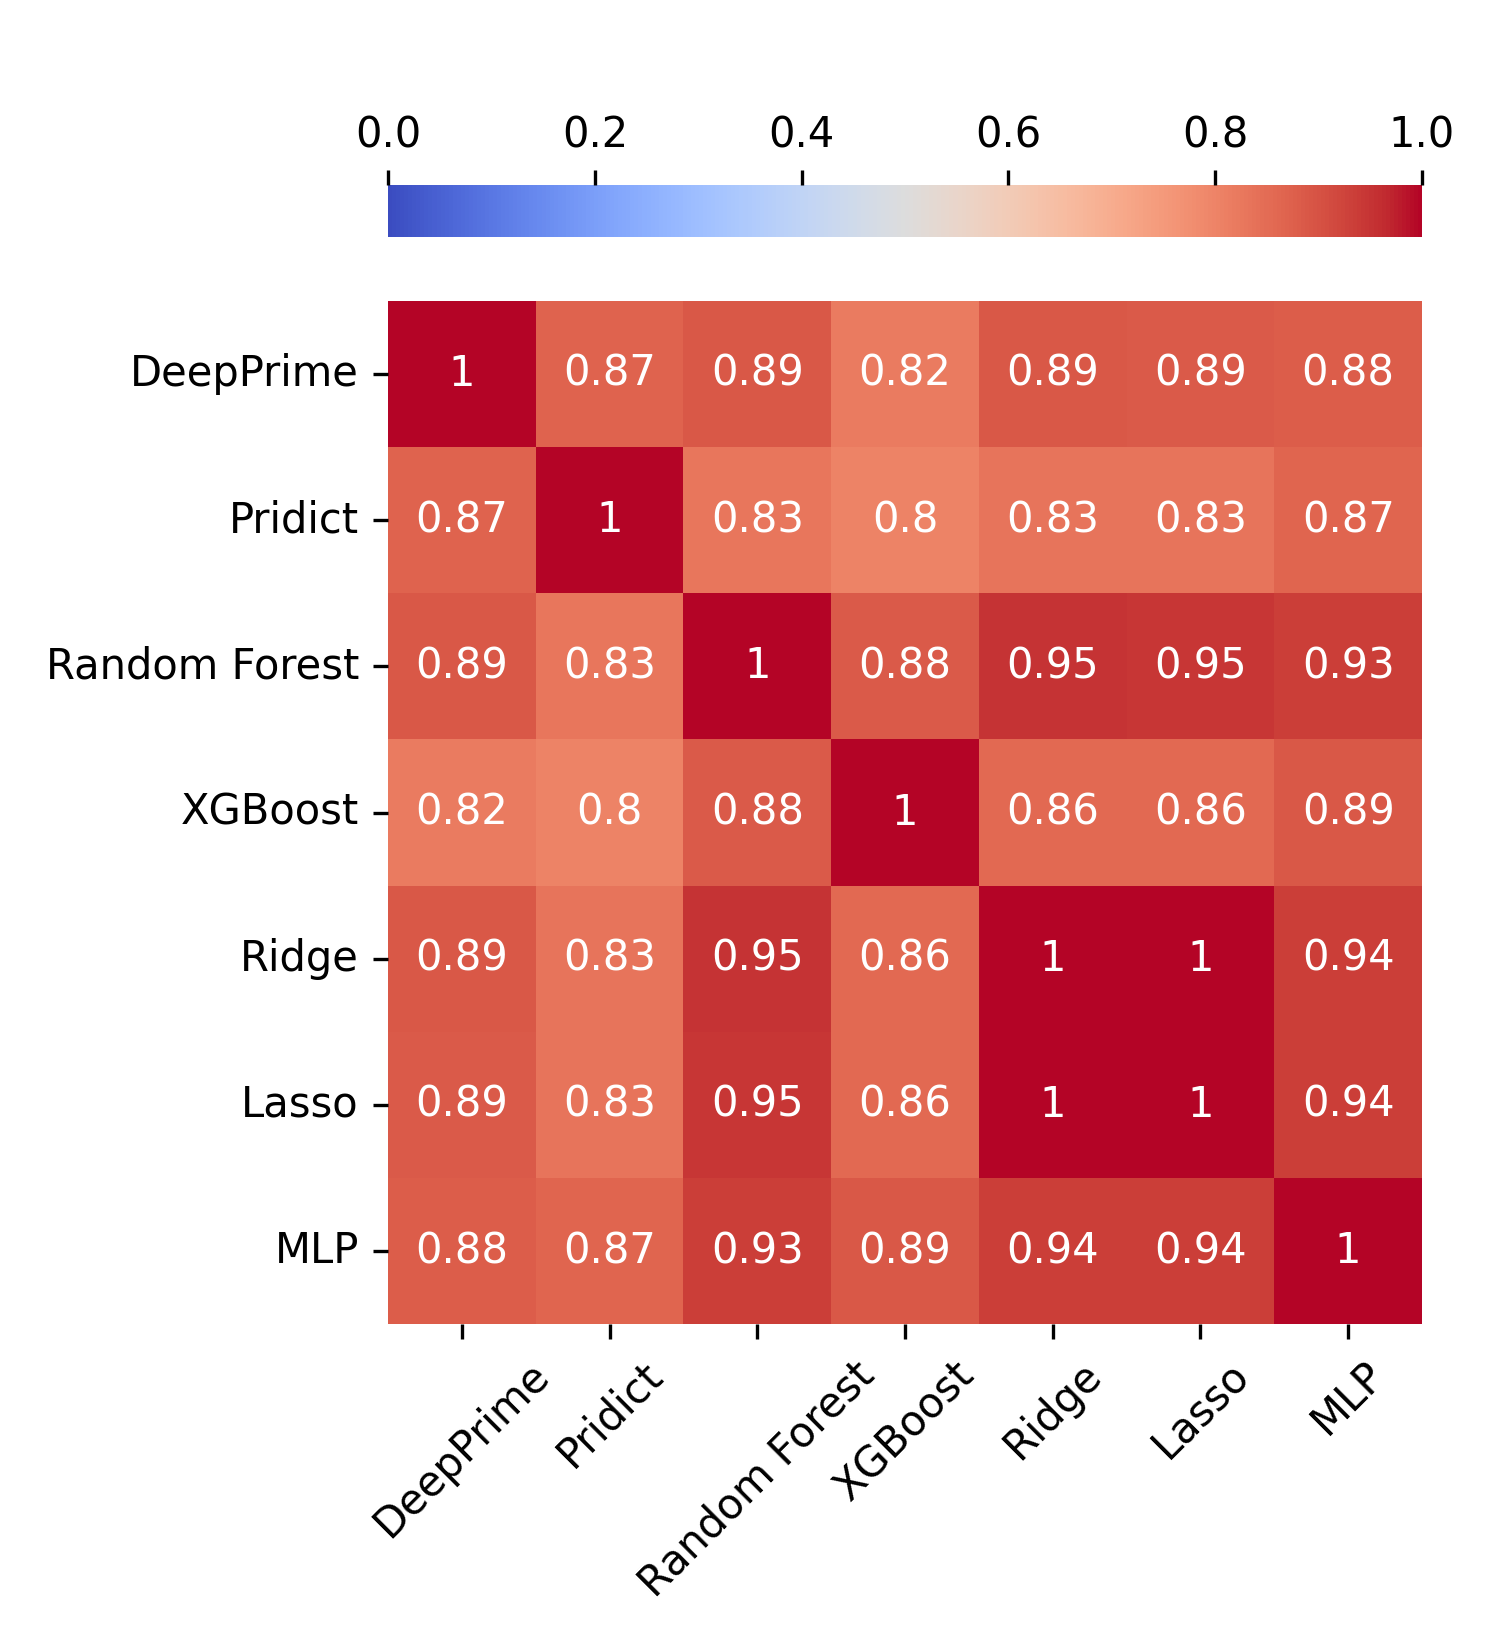
\includegraphics[width=0.49\textwidth]{error_correlation_pd-k562-pe2_pearson.png}
        % \caption{Pearson Correlation of the Error of the Individual Models}
        \label{fig:pearson-correlation-k562-pe2}
    }%
    \subfigure[][Spearman Correlation]{
        \centering
        \includegraphics[width=0.49\textwidth]{error_correlation_pd-k562-pe2_spearman.png}
        % \caption{Spearman Correlation of the Error of the Individual Models}
        \label{fig:spearman-correlation-k562-pe2}
    }
    \caption[Error Analysis of the Individual Models on PRIDICT K562 PE2 dataset]{Error Analysis of the Individual Models on the PRIDICT K562 PE2 dataset. \textbf{(a)}, \textbf{(b)}, and \textbf{(c)} are the same as \autoref{fig:error-analysis-adv-pe2}.}
    \label{fig:error-analysis-k562-pe2}
\end{figure}

\begin{figure}
    \centering
    \subfigure[][Error Distribution]{
        \centering
        \includegraphics[width=\textwidth]{error_comparison_pd-k562mlh1dn-pe2.png}
        % \caption{Error Distribution of the Individual Models}
        \label{fig:error-distribution-k562mlh1dn-pe2}
    }
    \subfigure[][Pearson Correlation]{
        \centering
        \includegraphics[width=0.49\textwidth]{error_correlation_pd-k562mlh1dn-pe2_pearson.png}
        % \caption{Pearson Correlation of the Error of the Individual Models}
        \label{fig:pearson-correlation-k562mlh1dn-pe2}
    }%
    \subfigure[][Spearman Correlation]{
        \centering
        \includegraphics[width=0.49\textwidth]{error_correlation_pd-k562mlh1dn-pe2_spearman.png}
        % \caption{Spearman Correlation of the Error of the Individual Models}
        \label{fig:spearman-correlation-k562mlh1dn-pe2}
    }
    \caption[Error Analysis of the Individual Models on PRIDICT K562 MLH1 DN PE2 dataset]{Error Analysis of the Individual Models on the PRIDICT K562 MLH1 DN PE2 dataset. \textbf{(a)}, \textbf{(b)}, and \textbf{(c)} are the same as \autoref{fig:error-analysis-adv-pe2}.}
    \label{fig:error-analysis-k562mlh1dn-pe2}
\end{figure}

\begin{figure}
    
\end{figure}

\newpage

\section{}


\printbibliography[heading=bibintoc,title={\bibtitle}]}


\end{document}